\documentclass{beamer}
\usepackage{eulervm}
%%%%%%%PACKAGES%%%%%%%%%
\usepackage[english]{babel}
\usepackage{amssymb,amsmath}
\usepackage[ansinew]{inputenc}
\usepackage{multimedia}
\usepackage{hyperref} 
\usepackage{color}
\definecolor{AliceBlue}{rgb}{0.94,0.97,1.00}
\definecolor{AntiqueWhite1}{rgb}{1.00,0.94,0.86}
\definecolor{AntiqueWhite2}{rgb}{0.93,0.87,0.80}
\definecolor{AntiqueWhite3}{rgb}{0.80,0.75,0.69}
\definecolor{AntiqueWhite4}{rgb}{0.55,0.51,0.47}
\definecolor{AntiqueWhite}{rgb}{0.98,0.92,0.84}
\definecolor{BlanchedAlmond}{rgb}{1.00,0.92,0.80}
\definecolor{BlueViolet}{rgb}{0.54,0.17,0.89}
\definecolor{CadetBlue1}{rgb}{0.60,0.96,1.00}
\definecolor{CadetBlue2}{rgb}{0.56,0.90,0.93}
\definecolor{CadetBlue3}{rgb}{0.48,0.77,0.80}
\definecolor{CadetBlue4}{rgb}{0.33,0.53,0.55}
\definecolor{CadetBlue}{rgb}{0.37,0.62,0.63}
\definecolor{CornflowerBlue}{rgb}{0.39,0.58,0.93}
\definecolor{DarkBlue}{rgb}{0.00,0.00,0.55}
\definecolor{DarkCyan}{rgb}{0.00,0.55,0.55}
\definecolor{DarkGoldenrod1}{rgb}{1.00,0.73,0.06}
\definecolor{DarkGoldenrod2}{rgb}{0.93,0.68,0.05}
\definecolor{DarkGoldenrod3}{rgb}{0.80,0.58,0.05}
\definecolor{DarkGoldenrod4}{rgb}{0.55,0.40,0.03}
\definecolor{DarkGoldenrod}{rgb}{0.72,0.53,0.04}
\definecolor{DarkGray}{rgb}{0.66,0.66,0.66}
\definecolor{DarkGreen}{rgb}{0.00,0.39,0.00}
\definecolor{DarkGrey}{rgb}{0.66,0.66,0.66}
\definecolor{DarkKhaki}{rgb}{0.74,0.72,0.42}
\definecolor{DarkMagenta}{rgb}{0.55,0.00,0.55}
\definecolor{DarkOliveGreen1}{rgb}{0.79,1.00,0.44}
\definecolor{DarkOliveGreen2}{rgb}{0.74,0.93,0.41}
\definecolor{DarkOliveGreen3}{rgb}{0.64,0.80,0.35}
\definecolor{DarkOliveGreen4}{rgb}{0.43,0.55,0.24}
\definecolor{DarkOliveGreen}{rgb}{0.33,0.42,0.18}
\definecolor{DarkOrange1}{rgb}{1.00,0.50,0.00}
\definecolor{DarkOrange2}{rgb}{0.93,0.46,0.00}
\definecolor{DarkOrange3}{rgb}{0.80,0.40,0.00}
\definecolor{DarkOrange4}{rgb}{0.55,0.27,0.00}
\definecolor{DarkOrange}{rgb}{1.00,0.55,0.00}
\definecolor{DarkOrchid1}{rgb}{0.75,0.24,1.00}
\definecolor{DarkOrchid2}{rgb}{0.70,0.23,0.93}
\definecolor{DarkOrchid3}{rgb}{0.60,0.20,0.80}
\definecolor{DarkOrchid4}{rgb}{0.41,0.13,0.55}
\definecolor{DarkOrchid}{rgb}{0.60,0.20,0.80}
\definecolor{DarkRed}{rgb}{0.55,0.00,0.00}
\definecolor{DarkSalmon}{rgb}{0.91,0.59,0.48}
\definecolor{DarkSeaGreen1}{rgb}{0.76,1.00,0.76}
\definecolor{DarkSeaGreen2}{rgb}{0.71,0.93,0.71}
\definecolor{DarkSeaGreen3}{rgb}{0.61,0.80,0.61}
\definecolor{DarkSeaGreen4}{rgb}{0.41,0.55,0.41}
\definecolor{DarkSeaGreen}{rgb}{0.56,0.74,0.56}
\definecolor{DarkSlateBlue}{rgb}{0.28,0.24,0.55}
\definecolor{DarkSlateGray1}{rgb}{0.59,1.00,1.00}
\definecolor{DarkSlateGray2}{rgb}{0.55,0.93,0.93}
\definecolor{DarkSlateGray3}{rgb}{0.47,0.80,0.80}
\definecolor{DarkSlateGray4}{rgb}{0.32,0.55,0.55}
\definecolor{DarkSlateGray}{rgb}{0.18,0.31,0.31}
\definecolor{DarkSlateGrey}{rgb}{0.18,0.31,0.31}
\definecolor{DarkTurquoise}{rgb}{0.00,0.81,0.82}
\definecolor{DarkViolet}{rgb}{0.58,0.00,0.83}
\definecolor{DeepPink1}{rgb}{1.00,0.08,0.58}
\definecolor{DeepPink2}{rgb}{0.93,0.07,0.54}
\definecolor{DeepPink3}{rgb}{0.80,0.06,0.46}
\definecolor{DeepPink4}{rgb}{0.55,0.04,0.31}
\definecolor{DeepPink}{rgb}{1.00,0.08,0.58}
\definecolor{DeepSkyBlue1}{rgb}{0.00,0.75,1.00}
\definecolor{DeepSkyBlue2}{rgb}{0.00,0.70,0.93}
\definecolor{DeepSkyBlue3}{rgb}{0.00,0.60,0.80}
\definecolor{DeepSkyBlue4}{rgb}{0.00,0.41,0.55}
\definecolor{DeepSkyBlue}{rgb}{0.00,0.75,1.00}
\definecolor{DimGray}{rgb}{0.41,0.41,0.41}
\definecolor{DimGrey}{rgb}{0.41,0.41,0.41}
\definecolor{DodgerBlue1}{rgb}{0.12,0.56,1.00}
\definecolor{DodgerBlue2}{rgb}{0.11,0.53,0.93}
\definecolor{DodgerBlue3}{rgb}{0.09,0.45,0.80}
\definecolor{DodgerBlue4}{rgb}{0.06,0.31,0.55}
\definecolor{DodgerBlue}{rgb}{0.12,0.56,1.00}
\definecolor{FloralWhite}{rgb}{1.00,0.98,0.94}
\definecolor{ForestGreen}{rgb}{0.13,0.55,0.13}
\definecolor{GhostWhite}{rgb}{0.97,0.97,1.00}
\definecolor{GreenYellow}{rgb}{0.68,1.00,0.18}
\definecolor{HotPink1}{rgb}{1.00,0.43,0.71}
\definecolor{HotPink2}{rgb}{0.93,0.42,0.65}
\definecolor{HotPink3}{rgb}{0.80,0.38,0.56}
\definecolor{HotPink4}{rgb}{0.55,0.23,0.38}
\definecolor{HotPink}{rgb}{1.00,0.41,0.71}
\definecolor{IndianRed1}{rgb}{1.00,0.42,0.42}
\definecolor{IndianRed2}{rgb}{0.93,0.39,0.39}
\definecolor{IndianRed3}{rgb}{0.80,0.33,0.33}
\definecolor{IndianRed4}{rgb}{0.55,0.23,0.23}
\definecolor{IndianRed}{rgb}{0.80,0.36,0.36}
\definecolor{LavenderBlush1}{rgb}{1.00,0.94,0.96}
\definecolor{LavenderBlush2}{rgb}{0.93,0.88,0.90}
\definecolor{LavenderBlush3}{rgb}{0.80,0.76,0.77}
\definecolor{LavenderBlush4}{rgb}{0.55,0.51,0.53}
\definecolor{LavenderBlush}{rgb}{1.00,0.94,0.96}
\definecolor{LawnGreen}{rgb}{0.49,0.99,0.00}
\definecolor{LemonChiffon1}{rgb}{1.00,0.98,0.80}
\definecolor{LemonChiffon2}{rgb}{0.93,0.91,0.75}
\definecolor{LemonChiffon3}{rgb}{0.80,0.79,0.65}
\definecolor{LemonChiffon4}{rgb}{0.55,0.54,0.44}
\definecolor{LemonChiffon}{rgb}{1.00,0.98,0.80}
\definecolor{LightBlue1}{rgb}{0.75,0.94,1.00}
\definecolor{LightBlue2}{rgb}{0.70,0.87,0.93}
\definecolor{LightBlue3}{rgb}{0.60,0.75,0.80}
\definecolor{LightBlue4}{rgb}{0.41,0.51,0.55}
\definecolor{LightBlue}{rgb}{0.68,0.85,0.90}
\definecolor{LightCoral}{rgb}{0.94,0.50,0.50}
\definecolor{LightCyan1}{rgb}{0.88,1.00,1.00}
\definecolor{LightCyan2}{rgb}{0.82,0.93,0.93}
\definecolor{LightCyan3}{rgb}{0.71,0.80,0.80}
\definecolor{LightCyan4}{rgb}{0.48,0.55,0.55}
\definecolor{LightCyan}{rgb}{0.88,1.00,1.00}
\definecolor{LightGoldenrod1}{rgb}{1.00,0.93,0.55}
\definecolor{LightGoldenrod2}{rgb}{0.93,0.86,0.51}
\definecolor{LightGoldenrod3}{rgb}{0.80,0.75,0.44}
\definecolor{LightGoldenrod4}{rgb}{0.55,0.51,0.30}
\definecolor{LightGoldenrodYellow}{rgb}{0.98,0.98,0.82}
\definecolor{LightGoldenrod}{rgb}{0.93,0.87,0.51}
\definecolor{LightGray}{rgb}{0.83,0.83,0.83}
\definecolor{LightGreen}{rgb}{0.56,0.93,0.56}
\definecolor{LightGrey}{rgb}{0.83,0.83,0.83}
\definecolor{LightPink1}{rgb}{1.00,0.68,0.73}
\definecolor{LightPink2}{rgb}{0.93,0.64,0.68}
\definecolor{LightPink3}{rgb}{0.80,0.55,0.58}
\definecolor{LightPink4}{rgb}{0.55,0.37,0.40}
\definecolor{LightPink}{rgb}{1.00,0.71,0.76}
\definecolor{LightSalmon1}{rgb}{1.00,0.63,0.48}
\definecolor{LightSalmon2}{rgb}{0.93,0.58,0.45}
\definecolor{LightSalmon3}{rgb}{0.80,0.51,0.38}
\definecolor{LightSalmon4}{rgb}{0.55,0.34,0.26}
\definecolor{LightSalmon}{rgb}{1.00,0.63,0.48}
\definecolor{LightSeaGreen}{rgb}{0.13,0.70,0.67}
\definecolor{LightSkyBlue1}{rgb}{0.69,0.89,1.00}
\definecolor{LightSkyBlue2}{rgb}{0.64,0.83,0.93}
\definecolor{LightSkyBlue3}{rgb}{0.55,0.71,0.80}
\definecolor{LightSkyBlue4}{rgb}{0.38,0.48,0.55}
\definecolor{LightSkyBlue}{rgb}{0.53,0.81,0.98}
\definecolor{LightSlateBlue}{rgb}{0.52,0.44,1.00}
\definecolor{LightSlateGray}{rgb}{0.47,0.53,0.60}
\definecolor{LightSlateGrey}{rgb}{0.47,0.53,0.60}
\definecolor{LightSteelBlue1}{rgb}{0.79,0.88,1.00}
\definecolor{LightSteelBlue2}{rgb}{0.74,0.82,0.93}
\definecolor{LightSteelBlue3}{rgb}{0.64,0.71,0.80}
\definecolor{LightSteelBlue4}{rgb}{0.43,0.48,0.55}
\definecolor{LightSteelBlue}{rgb}{0.69,0.77,0.87}
\definecolor{LightYellow1}{rgb}{1.00,1.00,0.88}
\definecolor{LightYellow2}{rgb}{0.93,0.93,0.82}
\definecolor{LightYellow3}{rgb}{0.80,0.80,0.71}
\definecolor{LightYellow4}{rgb}{0.55,0.55,0.48}
\definecolor{LightYellow}{rgb}{1.00,1.00,0.88}
\definecolor{LimeGreen}{rgb}{0.20,0.80,0.20}
\definecolor{MediumAquamarine}{rgb}{0.40,0.80,0.67}
\definecolor{MediumBlue}{rgb}{0.00,0.00,0.80}
\definecolor{MediumOrchid1}{rgb}{0.88,0.40,1.00}
\definecolor{MediumOrchid2}{rgb}{0.82,0.37,0.93}
\definecolor{MediumOrchid3}{rgb}{0.71,0.32,0.80}
\definecolor{MediumOrchid4}{rgb}{0.48,0.22,0.55}
\definecolor{MediumOrchid}{rgb}{0.73,0.33,0.83}
\definecolor{MediumPurple1}{rgb}{0.67,0.51,1.00}
\definecolor{MediumPurple2}{rgb}{0.62,0.47,0.93}
\definecolor{MediumPurple3}{rgb}{0.54,0.41,0.80}
\definecolor{MediumPurple4}{rgb}{0.36,0.28,0.55}
\definecolor{MediumPurple}{rgb}{0.58,0.44,0.86}
\definecolor{MediumSeaGreen}{rgb}{0.24,0.70,0.44}
\definecolor{MediumSlateBlue}{rgb}{0.48,0.41,0.93}
\definecolor{MediumSpringGreen}{rgb}{0.00,0.98,0.60}
\definecolor{MediumTurquoise}{rgb}{0.28,0.82,0.80}
\definecolor{MediumVioletRed}{rgb}{0.78,0.08,0.52}
\definecolor{MidnightBlue}{rgb}{0.10,0.10,0.44}
\definecolor{MintCream}{rgb}{0.96,1.00,0.98}
\definecolor{MistyRose1}{rgb}{1.00,0.89,0.88}
\definecolor{MistyRose2}{rgb}{0.93,0.84,0.82}
\definecolor{MistyRose3}{rgb}{0.80,0.72,0.71}
\definecolor{MistyRose4}{rgb}{0.55,0.49,0.48}
\definecolor{MistyRose}{rgb}{1.00,0.89,0.88}
\definecolor{NavajoWhite1}{rgb}{1.00,0.87,0.68}
\definecolor{NavajoWhite2}{rgb}{0.93,0.81,0.63}
\definecolor{NavajoWhite3}{rgb}{0.80,0.70,0.55}
\definecolor{NavajoWhite4}{rgb}{0.55,0.47,0.37}
\definecolor{NavajoWhite}{rgb}{1.00,0.87,0.68}
\definecolor{NavyBlue}{rgb}{0.00,0.00,0.50}
\definecolor{OldLace}{rgb}{0.99,0.96,0.90}
\definecolor{OliveDrab1}{rgb}{0.75,1.00,0.24}
\definecolor{OliveDrab2}{rgb}{0.70,0.93,0.23}
\definecolor{OliveDrab3}{rgb}{0.60,0.80,0.20}
\definecolor{OliveDrab4}{rgb}{0.41,0.55,0.13}
\definecolor{OliveDrab}{rgb}{0.42,0.56,0.14}
\definecolor{OrangeRed1}{rgb}{1.00,0.27,0.00}
\definecolor{OrangeRed2}{rgb}{0.93,0.25,0.00}
\definecolor{OrangeRed3}{rgb}{0.80,0.22,0.00}
\definecolor{OrangeRed4}{rgb}{0.55,0.15,0.00}
\definecolor{OrangeRed}{rgb}{1.00,0.27,0.00}
\definecolor{PaleGoldenrod}{rgb}{0.93,0.91,0.67}
\definecolor{PaleGreen1}{rgb}{0.60,1.00,0.60}
\definecolor{PaleGreen2}{rgb}{0.56,0.93,0.56}
\definecolor{PaleGreen3}{rgb}{0.49,0.80,0.49}
\definecolor{PaleGreen4}{rgb}{0.33,0.55,0.33}
\definecolor{PaleGreen}{rgb}{0.60,0.98,0.60}
\definecolor{PaleTurquoise1}{rgb}{0.73,1.00,1.00}
\definecolor{PaleTurquoise2}{rgb}{0.68,0.93,0.93}
\definecolor{PaleTurquoise3}{rgb}{0.59,0.80,0.80}
\definecolor{PaleTurquoise4}{rgb}{0.40,0.55,0.55}
\definecolor{PaleTurquoise}{rgb}{0.69,0.93,0.93}
\definecolor{PaleVioletRed1}{rgb}{1.00,0.51,0.67}
\definecolor{PaleVioletRed2}{rgb}{0.93,0.47,0.62}
\definecolor{PaleVioletRed3}{rgb}{0.80,0.41,0.54}
\definecolor{PaleVioletRed4}{rgb}{0.55,0.28,0.36}
\definecolor{PaleVioletRed}{rgb}{0.86,0.44,0.58}
\definecolor{PapayaWhip}{rgb}{1.00,0.94,0.84}
\definecolor{PeachPuff1}{rgb}{1.00,0.85,0.73}
\definecolor{PeachPuff2}{rgb}{0.93,0.80,0.68}
\definecolor{PeachPuff3}{rgb}{0.80,0.69,0.58}
\definecolor{PeachPuff4}{rgb}{0.55,0.47,0.40}
\definecolor{PeachPuff}{rgb}{1.00,0.85,0.73}
\definecolor{PowderBlue}{rgb}{0.69,0.88,0.90}
\definecolor{RosyBrown1}{rgb}{1.00,0.76,0.76}
\definecolor{RosyBrown2}{rgb}{0.93,0.71,0.71}
\definecolor{RosyBrown3}{rgb}{0.80,0.61,0.61}
\definecolor{RosyBrown4}{rgb}{0.55,0.41,0.41}
\definecolor{RosyBrown}{rgb}{0.74,0.56,0.56}
\definecolor{RoyalBlue1}{rgb}{0.28,0.46,1.00}
\definecolor{RoyalBlue2}{rgb}{0.26,0.43,0.93}
\definecolor{RoyalBlue3}{rgb}{0.23,0.37,0.80}
\definecolor{RoyalBlue4}{rgb}{0.15,0.25,0.55}
\definecolor{RoyalBlue}{rgb}{0.25,0.41,0.88}
\definecolor{SaddleBrown}{rgb}{0.55,0.27,0.07}
\definecolor{SandyBrown}{rgb}{0.96,0.64,0.38}
\definecolor{SeaGreen1}{rgb}{0.33,1.00,0.62}
\definecolor{SeaGreen2}{rgb}{0.31,0.93,0.58}
\definecolor{SeaGreen3}{rgb}{0.26,0.80,0.50}
\definecolor{SeaGreen4}{rgb}{0.18,0.55,0.34}
\definecolor{SeaGreen}{rgb}{0.18,0.55,0.34}
\definecolor{SkyBlue1}{rgb}{0.53,0.81,1.00}
\definecolor{SkyBlue2}{rgb}{0.49,0.75,0.93}
\definecolor{SkyBlue3}{rgb}{0.42,0.65,0.80}
\definecolor{SkyBlue4}{rgb}{0.29,0.44,0.55}
\definecolor{SkyBlue}{rgb}{0.53,0.81,0.92}
\definecolor{SlateBlue1}{rgb}{0.51,0.44,1.00}
\definecolor{SlateBlue2}{rgb}{0.48,0.40,0.93}
\definecolor{SlateBlue3}{rgb}{0.41,0.35,0.80}
\definecolor{SlateBlue4}{rgb}{0.28,0.24,0.55}
\definecolor{SlateBlue}{rgb}{0.42,0.35,0.80}
\definecolor{SlateGray1}{rgb}{0.78,0.89,1.00}
\definecolor{SlateGray2}{rgb}{0.73,0.83,0.93}
\definecolor{SlateGray3}{rgb}{0.62,0.71,0.80}
\definecolor{SlateGray4}{rgb}{0.42,0.48,0.55}
\definecolor{SlateGray}{rgb}{0.44,0.50,0.56}
\definecolor{SlateGrey}{rgb}{0.44,0.50,0.56}
\definecolor{SpringGreen1}{rgb}{0.00,1.00,0.50}
\definecolor{SpringGreen2}{rgb}{0.00,0.93,0.46}
\definecolor{SpringGreen3}{rgb}{0.00,0.80,0.40}
\definecolor{SpringGreen4}{rgb}{0.00,0.55,0.27}
\definecolor{SpringGreen}{rgb}{0.00,1.00,0.50}
\definecolor{SteelBlue1}{rgb}{0.39,0.72,1.00}
\definecolor{SteelBlue2}{rgb}{0.36,0.67,0.93}
\definecolor{SteelBlue3}{rgb}{0.31,0.58,0.80}
\definecolor{SteelBlue4}{rgb}{0.21,0.39,0.55}
\definecolor{SteelBlue}{rgb}{0.27,0.51,0.71}
\definecolor{VioletRed1}{rgb}{1.00,0.24,0.59}
\definecolor{VioletRed2}{rgb}{0.93,0.23,0.55}
\definecolor{VioletRed3}{rgb}{0.80,0.20,0.47}
\definecolor{VioletRed4}{rgb}{0.55,0.13,0.32}
\definecolor{VioletRed}{rgb}{0.82,0.13,0.56}
\definecolor{WhiteSmoke}{rgb}{0.96,0.96,0.96}
\definecolor{YellowGreen}{rgb}{0.60,0.80,0.20}
\definecolor{aliceblue}{rgb}{0.94,0.97,1.00}
\definecolor{antiquewhite}{rgb}{0.98,0.92,0.84}
\definecolor{aquamarine1}{rgb}{0.50,1.00,0.83}
\definecolor{aquamarine2}{rgb}{0.46,0.93,0.78}
\definecolor{aquamarine3}{rgb}{0.40,0.80,0.67}
\definecolor{aquamarine4}{rgb}{0.27,0.55,0.45}
\definecolor{aquamarine}{rgb}{0.50,1.00,0.83}
\definecolor{azure1}{rgb}{0.94,1.00,1.00}
\definecolor{azure2}{rgb}{0.88,0.93,0.93}
\definecolor{azure3}{rgb}{0.76,0.80,0.80}
\definecolor{azure4}{rgb}{0.51,0.55,0.55}
\definecolor{azure}{rgb}{0.94,1.00,1.00}
\definecolor{beige}{rgb}{0.96,0.96,0.86}
\definecolor{bisque1}{rgb}{1.00,0.89,0.77}
\definecolor{bisque2}{rgb}{0.93,0.84,0.72}
\definecolor{bisque3}{rgb}{0.80,0.72,0.62}
\definecolor{bisque4}{rgb}{0.55,0.49,0.42}
\definecolor{bisque}{rgb}{1.00,0.89,0.77}
\definecolor{black}{rgb}{0.00,0.00,0.00}
\definecolor{blanchedalmond}{rgb}{1.00,0.92,0.80}
\definecolor{blue1}{rgb}{0.00,0.00,1.00}
\definecolor{blue2}{rgb}{0.00,0.00,0.93}
\definecolor{blue3}{rgb}{0.00,0.00,0.80}
\definecolor{blue4}{rgb}{0.00,0.00,0.55}
\definecolor{blueviolet}{rgb}{0.54,0.17,0.89}
\definecolor{blue}{rgb}{0.00,0.00,1.00}
\definecolor{brown1}{rgb}{1.00,0.25,0.25}
\definecolor{brown2}{rgb}{0.93,0.23,0.23}
\definecolor{brown3}{rgb}{0.80,0.20,0.20}
\definecolor{brown4}{rgb}{0.55,0.14,0.14}
\definecolor{brown}{rgb}{0.65,0.16,0.16}
\definecolor{burlywood1}{rgb}{1.00,0.83,0.61}
\definecolor{burlywood2}{rgb}{0.93,0.77,0.57}
\definecolor{burlywood3}{rgb}{0.80,0.67,0.49}
\definecolor{burlywood4}{rgb}{0.55,0.45,0.33}
\definecolor{burlywood}{rgb}{0.87,0.72,0.53}
\definecolor{cadetblue}{rgb}{0.37,0.62,0.63}
\definecolor{chartreuse1}{rgb}{0.50,1.00,0.00}
\definecolor{chartreuse2}{rgb}{0.46,0.93,0.00}
\definecolor{chartreuse3}{rgb}{0.40,0.80,0.00}
\definecolor{chartreuse4}{rgb}{0.27,0.55,0.00}
\definecolor{chartreuse}{rgb}{0.50,1.00,0.00}
\definecolor{chocolate1}{rgb}{1.00,0.50,0.14}
\definecolor{chocolate2}{rgb}{0.93,0.46,0.13}
\definecolor{chocolate3}{rgb}{0.80,0.40,0.11}
\definecolor{chocolate4}{rgb}{0.55,0.27,0.07}
\definecolor{chocolate}{rgb}{0.82,0.41,0.12}
\definecolor{coral1}{rgb}{1.00,0.45,0.34}
\definecolor{coral2}{rgb}{0.93,0.42,0.31}
\definecolor{coral3}{rgb}{0.80,0.36,0.27}
\definecolor{coral4}{rgb}{0.55,0.24,0.18}
\definecolor{coral}{rgb}{1.00,0.50,0.31}
\definecolor{cornflowerblue}{rgb}{0.39,0.58,0.93}
\definecolor{cornsilk1}{rgb}{1.00,0.97,0.86}
\definecolor{cornsilk2}{rgb}{0.93,0.91,0.80}
\definecolor{cornsilk3}{rgb}{0.80,0.78,0.69}
\definecolor{cornsilk4}{rgb}{0.55,0.53,0.47}
\definecolor{cornsilk}{rgb}{1.00,0.97,0.86}
\definecolor{cyan1}{rgb}{0.00,1.00,1.00}
\definecolor{cyan2}{rgb}{0.00,0.93,0.93}
\definecolor{cyan3}{rgb}{0.00,0.80,0.80}
\definecolor{cyan4}{rgb}{0.00,0.55,0.55}
\definecolor{cyan}{rgb}{0.00,1.00,1.00}
\definecolor{darkblue}{rgb}{0.00,0.00,0.55}
\definecolor{darkcyan}{rgb}{0.00,0.55,0.55}
\definecolor{darkgoldenrod}{rgb}{0.72,0.53,0.04}
\definecolor{darkgray}{rgb}{0.66,0.66,0.66}
\definecolor{darkgreen}{rgb}{0.00,0.39,0.00}
\definecolor{darkgrey}{rgb}{0.66,0.66,0.66}
\definecolor{darkkhaki}{rgb}{0.74,0.72,0.42}
\definecolor{darkmagenta}{rgb}{0.55,0.00,0.55}
\definecolor{darkolive}{rgb}{0.33,0.42,0.18}
\definecolor{darkorange}{rgb}{1.00,0.55,0.00}
\definecolor{darkorchid}{rgb}{0.60,0.20,0.80}
\definecolor{darkred}{rgb}{0.55,0.00,0.00}
\definecolor{darksalmon}{rgb}{0.91,0.59,0.48}
\definecolor{darksea}{rgb}{0.56,0.74,0.56}
\definecolor{darkslate}{rgb}{0.18,0.31,0.31}
\definecolor{darkslate}{rgb}{0.18,0.31,0.31}
\definecolor{darkslate}{rgb}{0.28,0.24,0.55}
\definecolor{darkturquoise}{rgb}{0.00,0.81,0.82}
\definecolor{darkviolet}{rgb}{0.58,0.00,0.83}
\definecolor{deeppink}{rgb}{1.00,0.08,0.58}
\definecolor{deepsky}{rgb}{0.00,0.75,1.00}
\definecolor{dimgray}{rgb}{0.41,0.41,0.41}
\definecolor{dimgrey}{rgb}{0.41,0.41,0.41}
\definecolor{dodgerblue}{rgb}{0.12,0.56,1.00}
\definecolor{firebrick1}{rgb}{1.00,0.19,0.19}
\definecolor{firebrick2}{rgb}{0.93,0.17,0.17}
\definecolor{firebrick3}{rgb}{0.80,0.15,0.15}
\definecolor{firebrick4}{rgb}{0.55,0.10,0.10}
\definecolor{firebrick}{rgb}{0.70,0.13,0.13}
\definecolor{floralwhite}{rgb}{1.00,0.98,0.94}
\definecolor{forestgreen}{rgb}{0.13,0.55,0.13}
\definecolor{gainsboro}{rgb}{0.86,0.86,0.86}
\definecolor{ghostwhite}{rgb}{0.97,0.97,1.00}
\definecolor{gold1}{rgb}{1.00,0.84,0.00}
\definecolor{gold2}{rgb}{0.93,0.79,0.00}
\definecolor{gold3}{rgb}{0.80,0.68,0.00}
\definecolor{gold4}{rgb}{0.55,0.46,0.00}
\definecolor{goldenrod1}{rgb}{1.00,0.76,0.15}
\definecolor{goldenrod2}{rgb}{0.93,0.71,0.13}
\definecolor{goldenrod3}{rgb}{0.80,0.61,0.11}
\definecolor{goldenrod4}{rgb}{0.55,0.41,0.08}
\definecolor{goldenrod}{rgb}{0.85,0.65,0.13}
\definecolor{gold}{rgb}{1.00,0.84,0.00}
\definecolor{gray0}{rgb}{0.00,0.00,0.00}
\definecolor{gray100}{rgb}{1.00,1.00,1.00}
\definecolor{gray10}{rgb}{0.10,0.10,0.10}
\definecolor{gray11}{rgb}{0.11,0.11,0.11}
\definecolor{gray12}{rgb}{0.12,0.12,0.12}
\definecolor{gray13}{rgb}{0.13,0.13,0.13}
\definecolor{gray14}{rgb}{0.14,0.14,0.14}
\definecolor{gray15}{rgb}{0.15,0.15,0.15}
\definecolor{gray16}{rgb}{0.16,0.16,0.16}
\definecolor{gray17}{rgb}{0.17,0.17,0.17}
\definecolor{gray18}{rgb}{0.18,0.18,0.18}
\definecolor{gray19}{rgb}{0.19,0.19,0.19}
\definecolor{gray1}{rgb}{0.01,0.01,0.01}
\definecolor{gray20}{rgb}{0.20,0.20,0.20}
\definecolor{gray21}{rgb}{0.21,0.21,0.21}
\definecolor{gray22}{rgb}{0.22,0.22,0.22}
\definecolor{gray23}{rgb}{0.23,0.23,0.23}
\definecolor{gray24}{rgb}{0.24,0.24,0.24}
\definecolor{gray25}{rgb}{0.25,0.25,0.25}
\definecolor{gray26}{rgb}{0.26,0.26,0.26}
\definecolor{gray27}{rgb}{0.27,0.27,0.27}
\definecolor{gray28}{rgb}{0.28,0.28,0.28}
\definecolor{gray29}{rgb}{0.29,0.29,0.29}
\definecolor{gray2}{rgb}{0.02,0.02,0.02}
\definecolor{gray30}{rgb}{0.30,0.30,0.30}
\definecolor{gray31}{rgb}{0.31,0.31,0.31}
\definecolor{gray32}{rgb}{0.32,0.32,0.32}
\definecolor{gray33}{rgb}{0.33,0.33,0.33}
\definecolor{gray34}{rgb}{0.34,0.34,0.34}
\definecolor{gray35}{rgb}{0.35,0.35,0.35}
\definecolor{gray36}{rgb}{0.36,0.36,0.36}
\definecolor{gray37}{rgb}{0.37,0.37,0.37}
\definecolor{gray38}{rgb}{0.38,0.38,0.38}
\definecolor{gray39}{rgb}{0.39,0.39,0.39}
\definecolor{gray3}{rgb}{0.03,0.03,0.03}
\definecolor{gray40}{rgb}{0.40,0.40,0.40}
\definecolor{gray41}{rgb}{0.41,0.41,0.41}
\definecolor{gray42}{rgb}{0.42,0.42,0.42}
\definecolor{gray43}{rgb}{0.43,0.43,0.43}
\definecolor{gray44}{rgb}{0.44,0.44,0.44}
\definecolor{gray45}{rgb}{0.45,0.45,0.45}
\definecolor{gray46}{rgb}{0.46,0.46,0.46}
\definecolor{gray47}{rgb}{0.47,0.47,0.47}
\definecolor{gray48}{rgb}{0.48,0.48,0.48}
\definecolor{gray49}{rgb}{0.49,0.49,0.49}
\definecolor{gray4}{rgb}{0.04,0.04,0.04}
\definecolor{gray50}{rgb}{0.50,0.50,0.50}
\definecolor{gray51}{rgb}{0.51,0.51,0.51}
\definecolor{gray52}{rgb}{0.52,0.52,0.52}
\definecolor{gray53}{rgb}{0.53,0.53,0.53}
\definecolor{gray54}{rgb}{0.54,0.54,0.54}
\definecolor{gray55}{rgb}{0.55,0.55,0.55}
\definecolor{gray56}{rgb}{0.56,0.56,0.56}
\definecolor{gray57}{rgb}{0.57,0.57,0.57}
\definecolor{gray58}{rgb}{0.58,0.58,0.58}
\definecolor{gray59}{rgb}{0.59,0.59,0.59}
\definecolor{gray5}{rgb}{0.05,0.05,0.05}
\definecolor{gray60}{rgb}{0.60,0.60,0.60}
\definecolor{gray61}{rgb}{0.61,0.61,0.61}
\definecolor{gray62}{rgb}{0.62,0.62,0.62}
\definecolor{gray63}{rgb}{0.63,0.63,0.63}
\definecolor{gray64}{rgb}{0.64,0.64,0.64}
\definecolor{gray65}{rgb}{0.65,0.65,0.65}
\definecolor{gray66}{rgb}{0.66,0.66,0.66}
\definecolor{gray67}{rgb}{0.67,0.67,0.67}
\definecolor{gray68}{rgb}{0.68,0.68,0.68}
\definecolor{gray69}{rgb}{0.69,0.69,0.69}
\definecolor{gray6}{rgb}{0.06,0.06,0.06}
\definecolor{gray70}{rgb}{0.70,0.70,0.70}
\definecolor{gray71}{rgb}{0.71,0.71,0.71}
\definecolor{gray72}{rgb}{0.72,0.72,0.72}
\definecolor{gray73}{rgb}{0.73,0.73,0.73}
\definecolor{gray74}{rgb}{0.74,0.74,0.74}
\definecolor{gray75}{rgb}{0.75,0.75,0.75}
\definecolor{gray76}{rgb}{0.76,0.76,0.76}
\definecolor{gray77}{rgb}{0.77,0.77,0.77}
\definecolor{gray78}{rgb}{0.78,0.78,0.78}
\definecolor{gray79}{rgb}{0.79,0.79,0.79}
\definecolor{gray7}{rgb}{0.07,0.07,0.07}
\definecolor{gray80}{rgb}{0.80,0.80,0.80}
\definecolor{gray81}{rgb}{0.81,0.81,0.81}
\definecolor{gray82}{rgb}{0.82,0.82,0.82}
\definecolor{gray83}{rgb}{0.83,0.83,0.83}
\definecolor{gray84}{rgb}{0.84,0.84,0.84}
\definecolor{gray85}{rgb}{0.85,0.85,0.85}
\definecolor{gray86}{rgb}{0.86,0.86,0.86}
\definecolor{gray87}{rgb}{0.87,0.87,0.87}
\definecolor{gray88}{rgb}{0.88,0.88,0.88}
\definecolor{gray89}{rgb}{0.89,0.89,0.89}
\definecolor{gray8}{rgb}{0.08,0.08,0.08}
\definecolor{gray90}{rgb}{0.90,0.90,0.90}
\definecolor{gray91}{rgb}{0.91,0.91,0.91}
\definecolor{gray92}{rgb}{0.92,0.92,0.92}
\definecolor{gray93}{rgb}{0.93,0.93,0.93}
\definecolor{gray94}{rgb}{0.94,0.94,0.94}
\definecolor{gray95}{rgb}{0.95,0.95,0.95}
\definecolor{gray96}{rgb}{0.96,0.96,0.96}
\definecolor{gray97}{rgb}{0.97,0.97,0.97}
\definecolor{gray98}{rgb}{0.98,0.98,0.98}
\definecolor{gray99}{rgb}{0.99,0.99,0.99}
\definecolor{gray9}{rgb}{0.09,0.09,0.09}
\definecolor{gray}{rgb}{0.75,0.75,0.75}
\definecolor{green1}{rgb}{0.00,1.00,0.00}
\definecolor{green2}{rgb}{0.00,0.93,0.00}
\definecolor{green3}{rgb}{0.00,0.80,0.00}
\definecolor{green4}{rgb}{0.00,0.55,0.00}
\definecolor{greenyellow}{rgb}{0.68,1.00,0.18}
\definecolor{green}{rgb}{0.00,1.00,0.00}
\definecolor{grey0}{rgb}{0.00,0.00,0.00}
\definecolor{grey100}{rgb}{1.00,1.00,1.00}
\definecolor{grey10}{rgb}{0.10,0.10,0.10}
\definecolor{grey11}{rgb}{0.11,0.11,0.11}
\definecolor{grey12}{rgb}{0.12,0.12,0.12}
\definecolor{grey13}{rgb}{0.13,0.13,0.13}
\definecolor{grey14}{rgb}{0.14,0.14,0.14}
\definecolor{grey15}{rgb}{0.15,0.15,0.15}
\definecolor{grey16}{rgb}{0.16,0.16,0.16}
\definecolor{grey17}{rgb}{0.17,0.17,0.17}
\definecolor{grey18}{rgb}{0.18,0.18,0.18}
\definecolor{grey19}{rgb}{0.19,0.19,0.19}
\definecolor{grey1}{rgb}{0.01,0.01,0.01}
\definecolor{grey20}{rgb}{0.20,0.20,0.20}
\definecolor{grey21}{rgb}{0.21,0.21,0.21}
\definecolor{grey22}{rgb}{0.22,0.22,0.22}
\definecolor{grey23}{rgb}{0.23,0.23,0.23}
\definecolor{grey24}{rgb}{0.24,0.24,0.24}
\definecolor{grey25}{rgb}{0.25,0.25,0.25}
\definecolor{grey26}{rgb}{0.26,0.26,0.26}
\definecolor{grey27}{rgb}{0.27,0.27,0.27}
\definecolor{grey28}{rgb}{0.28,0.28,0.28}
\definecolor{grey29}{rgb}{0.29,0.29,0.29}
\definecolor{grey2}{rgb}{0.02,0.02,0.02}
\definecolor{grey30}{rgb}{0.30,0.30,0.30}
\definecolor{grey31}{rgb}{0.31,0.31,0.31}
\definecolor{grey32}{rgb}{0.32,0.32,0.32}
\definecolor{grey33}{rgb}{0.33,0.33,0.33}
\definecolor{grey34}{rgb}{0.34,0.34,0.34}
\definecolor{grey35}{rgb}{0.35,0.35,0.35}
\definecolor{grey36}{rgb}{0.36,0.36,0.36}
\definecolor{grey37}{rgb}{0.37,0.37,0.37}
\definecolor{grey38}{rgb}{0.38,0.38,0.38}
\definecolor{grey39}{rgb}{0.39,0.39,0.39}
\definecolor{grey3}{rgb}{0.03,0.03,0.03}
\definecolor{grey40}{rgb}{0.40,0.40,0.40}
\definecolor{grey41}{rgb}{0.41,0.41,0.41}
\definecolor{grey42}{rgb}{0.42,0.42,0.42}
\definecolor{grey43}{rgb}{0.43,0.43,0.43}
\definecolor{grey44}{rgb}{0.44,0.44,0.44}
\definecolor{grey45}{rgb}{0.45,0.45,0.45}
\definecolor{grey46}{rgb}{0.46,0.46,0.46}
\definecolor{grey47}{rgb}{0.47,0.47,0.47}
\definecolor{grey48}{rgb}{0.48,0.48,0.48}
\definecolor{grey49}{rgb}{0.49,0.49,0.49}
\definecolor{grey4}{rgb}{0.04,0.04,0.04}
\definecolor{grey50}{rgb}{0.50,0.50,0.50}
\definecolor{grey51}{rgb}{0.51,0.51,0.51}
\definecolor{grey52}{rgb}{0.52,0.52,0.52}
\definecolor{grey53}{rgb}{0.53,0.53,0.53}
\definecolor{grey54}{rgb}{0.54,0.54,0.54}
\definecolor{grey55}{rgb}{0.55,0.55,0.55}
\definecolor{grey56}{rgb}{0.56,0.56,0.56}
\definecolor{grey57}{rgb}{0.57,0.57,0.57}
\definecolor{grey58}{rgb}{0.58,0.58,0.58}
\definecolor{grey59}{rgb}{0.59,0.59,0.59}
\definecolor{grey5}{rgb}{0.05,0.05,0.05}
\definecolor{grey60}{rgb}{0.60,0.60,0.60}
\definecolor{grey61}{rgb}{0.61,0.61,0.61}
\definecolor{grey62}{rgb}{0.62,0.62,0.62}
\definecolor{grey63}{rgb}{0.63,0.63,0.63}
\definecolor{grey64}{rgb}{0.64,0.64,0.64}
\definecolor{grey65}{rgb}{0.65,0.65,0.65}
\definecolor{grey66}{rgb}{0.66,0.66,0.66}
\definecolor{grey67}{rgb}{0.67,0.67,0.67}
\definecolor{grey68}{rgb}{0.68,0.68,0.68}
\definecolor{grey69}{rgb}{0.69,0.69,0.69}
\definecolor{grey6}{rgb}{0.06,0.06,0.06}
\definecolor{grey70}{rgb}{0.70,0.70,0.70}
\definecolor{grey71}{rgb}{0.71,0.71,0.71}
\definecolor{grey72}{rgb}{0.72,0.72,0.72}
\definecolor{grey73}{rgb}{0.73,0.73,0.73}
\definecolor{grey74}{rgb}{0.74,0.74,0.74}
\definecolor{grey75}{rgb}{0.75,0.75,0.75}
\definecolor{grey76}{rgb}{0.76,0.76,0.76}
\definecolor{grey77}{rgb}{0.77,0.77,0.77}
\definecolor{grey78}{rgb}{0.78,0.78,0.78}
\definecolor{grey79}{rgb}{0.79,0.79,0.79}
\definecolor{grey7}{rgb}{0.07,0.07,0.07}
\definecolor{grey80}{rgb}{0.80,0.80,0.80}
\definecolor{grey81}{rgb}{0.81,0.81,0.81}
\definecolor{grey82}{rgb}{0.82,0.82,0.82}
\definecolor{grey83}{rgb}{0.83,0.83,0.83}
\definecolor{grey84}{rgb}{0.84,0.84,0.84}
\definecolor{grey85}{rgb}{0.85,0.85,0.85}
\definecolor{grey86}{rgb}{0.86,0.86,0.86}
\definecolor{grey87}{rgb}{0.87,0.87,0.87}
\definecolor{grey88}{rgb}{0.88,0.88,0.88}
\definecolor{grey89}{rgb}{0.89,0.89,0.89}
\definecolor{grey8}{rgb}{0.08,0.08,0.08}
\definecolor{grey90}{rgb}{0.90,0.90,0.90}
\definecolor{grey91}{rgb}{0.91,0.91,0.91}
\definecolor{grey92}{rgb}{0.92,0.92,0.92}
\definecolor{grey93}{rgb}{0.93,0.93,0.93}
\definecolor{grey94}{rgb}{0.94,0.94,0.94}
\definecolor{grey95}{rgb}{0.95,0.95,0.95}
\definecolor{grey96}{rgb}{0.96,0.96,0.96}
\definecolor{grey97}{rgb}{0.97,0.97,0.97}
\definecolor{grey98}{rgb}{0.98,0.98,0.98}
\definecolor{grey99}{rgb}{0.99,0.99,0.99}
\definecolor{grey9}{rgb}{0.09,0.09,0.09}
\definecolor{grey}{rgb}{0.75,0.75,0.75}
\definecolor{honeydew1}{rgb}{0.94,1.00,0.94}
\definecolor{honeydew2}{rgb}{0.88,0.93,0.88}
\definecolor{honeydew3}{rgb}{0.76,0.80,0.76}
\definecolor{honeydew4}{rgb}{0.51,0.55,0.51}
\definecolor{honeydew}{rgb}{0.94,1.00,0.94}
\definecolor{hotpink}{rgb}{1.00,0.41,0.71}
\definecolor{indianred}{rgb}{0.80,0.36,0.36}
\definecolor{ivory1}{rgb}{1.00,1.00,0.94}
\definecolor{ivory2}{rgb}{0.93,0.93,0.88}
\definecolor{ivory3}{rgb}{0.80,0.80,0.76}
\definecolor{ivory4}{rgb}{0.55,0.55,0.51}
\definecolor{ivory}{rgb}{1.00,1.00,0.94}
\definecolor{khaki1}{rgb}{1.00,0.96,0.56}
\definecolor{khaki2}{rgb}{0.93,0.90,0.52}
\definecolor{khaki3}{rgb}{0.80,0.78,0.45}
\definecolor{khaki4}{rgb}{0.55,0.53,0.31}
\definecolor{khaki}{rgb}{0.94,0.90,0.55}
\definecolor{lavenderblush}{rgb}{1.00,0.94,0.96}
\definecolor{lavender}{rgb}{0.90,0.90,0.98}
\definecolor{lawngreen}{rgb}{0.49,0.99,0.00}
\definecolor{lemonchiffon}{rgb}{1.00,0.98,0.80}
\definecolor{lightblue}{rgb}{0.68,0.85,0.90}
\definecolor{lightcoral}{rgb}{0.94,0.50,0.50}
\definecolor{lightcyan}{rgb}{0.88,1.00,1.00}
\definecolor{lightgoldenrod}{rgb}{0.93,0.87,0.51}
\definecolor{lightgoldenrod}{rgb}{0.98,0.98,0.82}
\definecolor{lightgray}{rgb}{0.83,0.83,0.83}
\definecolor{lightgreen}{rgb}{0.56,0.93,0.56}
\definecolor{lightgrey}{rgb}{0.83,0.83,0.83}
\definecolor{lightpink}{rgb}{1.00,0.71,0.76}
\definecolor{lightsalmon}{rgb}{1.00,0.63,0.48}
\definecolor{lightsea}{rgb}{0.13,0.70,0.67}
\definecolor{lightsky}{rgb}{0.53,0.81,0.98}
\definecolor{lightslate}{rgb}{0.47,0.53,0.60}
\definecolor{lightslate}{rgb}{0.47,0.53,0.60}
\definecolor{lightslate}{rgb}{0.52,0.44,1.00}
\definecolor{lightsteel}{rgb}{0.69,0.77,0.87}
\definecolor{lightyellow}{rgb}{1.00,1.00,0.88}
\definecolor{limegreen}{rgb}{0.20,0.80,0.20}
\definecolor{linen}{rgb}{0.98,0.94,0.90}
\definecolor{magenta1}{rgb}{1.00,0.00,1.00}
\definecolor{magenta2}{rgb}{0.93,0.00,0.93}
\definecolor{magenta3}{rgb}{0.80,0.00,0.80}
\definecolor{magenta4}{rgb}{0.55,0.00,0.55}
\definecolor{magenta}{rgb}{1.00,0.00,1.00}
\definecolor{maroon1}{rgb}{1.00,0.20,0.70}
\definecolor{maroon2}{rgb}{0.93,0.19,0.65}
\definecolor{maroon3}{rgb}{0.80,0.16,0.56}
\definecolor{maroon4}{rgb}{0.55,0.11,0.38}
\definecolor{maroon}{rgb}{0.69,0.19,0.38}
\definecolor{mediumaquamarine}{rgb}{0.40,0.80,0.67}
\definecolor{mediumblue}{rgb}{0.00,0.00,0.80}
\definecolor{mediumorchid}{rgb}{0.73,0.33,0.83}
\definecolor{mediumpurple}{rgb}{0.58,0.44,0.86}
\definecolor{mediumsea}{rgb}{0.24,0.70,0.44}
\definecolor{mediumslate}{rgb}{0.48,0.41,0.93}
\definecolor{mediumspring}{rgb}{0.00,0.98,0.60}
\definecolor{mediumturquoise}{rgb}{0.28,0.82,0.80}
\definecolor{mediumviolet}{rgb}{0.78,0.08,0.52}
\definecolor{midnightblue}{rgb}{0.10,0.10,0.44}
\definecolor{mintcream}{rgb}{0.96,1.00,0.98}
\definecolor{mistyrose}{rgb}{1.00,0.89,0.88}
\definecolor{moccasin}{rgb}{1.00,0.89,0.71}
\definecolor{navajowhite}{rgb}{1.00,0.87,0.68}
\definecolor{navyblue}{rgb}{0.00,0.00,0.50}
\definecolor{navy}{rgb}{0.00,0.00,0.50}
\definecolor{oldlace}{rgb}{0.99,0.96,0.90}
\definecolor{olivedrab}{rgb}{0.42,0.56,0.14}
\definecolor{orange1}{rgb}{1.00,0.65,0.00}
\definecolor{orange2}{rgb}{0.93,0.60,0.00}
\definecolor{orange3}{rgb}{0.80,0.52,0.00}
\definecolor{orange4}{rgb}{0.55,0.35,0.00}
\definecolor{orangered}{rgb}{1.00,0.27,0.00}
\definecolor{orange}{rgb}{1.00,0.65,0.00}
\definecolor{orchid1}{rgb}{1.00,0.51,0.98}
\definecolor{orchid2}{rgb}{0.93,0.48,0.91}
\definecolor{orchid3}{rgb}{0.80,0.41,0.79}
\definecolor{orchid4}{rgb}{0.55,0.28,0.54}
\definecolor{orchid}{rgb}{0.85,0.44,0.84}
\definecolor{palegoldenrod}{rgb}{0.93,0.91,0.67}
\definecolor{palegreen}{rgb}{0.60,0.98,0.60}
\definecolor{paleturquoise}{rgb}{0.69,0.93,0.93}
\definecolor{paleviolet}{rgb}{0.86,0.44,0.58}
\definecolor{papayawhip}{rgb}{1.00,0.94,0.84}
\definecolor{peachpuff}{rgb}{1.00,0.85,0.73}
\definecolor{peru}{rgb}{0.80,0.52,0.25}
\definecolor{pink1}{rgb}{1.00,0.71,0.77}
\definecolor{pink2}{rgb}{0.93,0.66,0.72}
\definecolor{pink3}{rgb}{0.80,0.57,0.62}
\definecolor{pink4}{rgb}{0.55,0.39,0.42}
\definecolor{pink}{rgb}{1.00,0.75,0.80}
\definecolor{plum1}{rgb}{1.00,0.73,1.00}
\definecolor{plum2}{rgb}{0.93,0.68,0.93}
\definecolor{plum3}{rgb}{0.80,0.59,0.80}
\definecolor{plum4}{rgb}{0.55,0.40,0.55}
\definecolor{plum}{rgb}{0.87,0.63,0.87}
\definecolor{powderblue}{rgb}{0.69,0.88,0.90}
\definecolor{purple1}{rgb}{0.61,0.19,1.00}
\definecolor{purple2}{rgb}{0.57,0.17,0.93}
\definecolor{purple3}{rgb}{0.49,0.15,0.80}
\definecolor{purple4}{rgb}{0.33,0.10,0.55}
\definecolor{purple}{rgb}{0.63,0.13,0.94}
\definecolor{red1}{rgb}{1.00,0.00,0.00}
\definecolor{red2}{rgb}{0.93,0.00,0.00}
\definecolor{red3}{rgb}{0.80,0.00,0.00}
\definecolor{red4}{rgb}{0.55,0.00,0.00}
\definecolor{red}{rgb}{1.00,0.00,0.00}
\definecolor{rosybrown}{rgb}{0.74,0.56,0.56}
\definecolor{royalblue}{rgb}{0.25,0.41,0.88}
\definecolor{saddlebrown}{rgb}{0.55,0.27,0.07}
\definecolor{salmon1}{rgb}{1.00,0.55,0.41}
\definecolor{salmon2}{rgb}{0.93,0.51,0.38}
\definecolor{salmon3}{rgb}{0.80,0.44,0.33}
\definecolor{salmon4}{rgb}{0.55,0.30,0.22}
\definecolor{salmon}{rgb}{0.98,0.50,0.45}
\definecolor{sandybrown}{rgb}{0.96,0.64,0.38}
\definecolor{seagreen}{rgb}{0.18,0.55,0.34}
\definecolor{seashell1}{rgb}{1.00,0.96,0.93}
\definecolor{seashell2}{rgb}{0.93,0.90,0.87}
\definecolor{seashell3}{rgb}{0.80,0.77,0.75}
\definecolor{seashell4}{rgb}{0.55,0.53,0.51}
\definecolor{seashell}{rgb}{1.00,0.96,0.93}
\definecolor{sienna1}{rgb}{1.00,0.51,0.28}
\definecolor{sienna2}{rgb}{0.93,0.47,0.26}
\definecolor{sienna3}{rgb}{0.80,0.41,0.22}
\definecolor{sienna4}{rgb}{0.55,0.28,0.15}
\definecolor{sienna}{rgb}{0.63,0.32,0.18}
\definecolor{skyblue}{rgb}{0.53,0.81,0.92}
\definecolor{slateblue}{rgb}{0.42,0.35,0.80}
\definecolor{slategray}{rgb}{0.44,0.50,0.56}
\definecolor{slategrey}{rgb}{0.44,0.50,0.56}
\definecolor{snow1}{rgb}{1.00,0.98,0.98}
\definecolor{snow2}{rgb}{0.93,0.91,0.91}
\definecolor{snow3}{rgb}{0.80,0.79,0.79}
\definecolor{snow4}{rgb}{0.55,0.54,0.54}
\definecolor{snow}{rgb}{1.00,0.98,0.98}
\definecolor{springgreen}{rgb}{0.00,1.00,0.50}
\definecolor{steelblue}{rgb}{0.27,0.51,0.71}
\definecolor{tan1}{rgb}{1.00,0.65,0.31}
\definecolor{tan2}{rgb}{0.93,0.60,0.29}
\definecolor{tan3}{rgb}{0.80,0.52,0.25}
\definecolor{tan4}{rgb}{0.55,0.35,0.17}
\definecolor{tan}{rgb}{0.82,0.71,0.55}
\definecolor{thistle1}{rgb}{1.00,0.88,1.00}
\definecolor{thistle2}{rgb}{0.93,0.82,0.93}
\definecolor{thistle3}{rgb}{0.80,0.71,0.80}
\definecolor{thistle4}{rgb}{0.55,0.48,0.55}
\definecolor{thistle}{rgb}{0.85,0.75,0.85}
\definecolor{tomato1}{rgb}{1.00,0.39,0.28}
\definecolor{tomato2}{rgb}{0.93,0.36,0.26}
\definecolor{tomato3}{rgb}{0.80,0.31,0.22}
\definecolor{tomato4}{rgb}{0.55,0.21,0.15}
\definecolor{tomato}{rgb}{1.00,0.39,0.28}
\definecolor{turquoise1}{rgb}{0.00,0.96,1.00}
\definecolor{turquoise2}{rgb}{0.00,0.90,0.93}
\definecolor{turquoise3}{rgb}{0.00,0.77,0.80}
\definecolor{turquoise4}{rgb}{0.00,0.53,0.55}
\definecolor{turquoise}{rgb}{0.25,0.88,0.82}
\definecolor{violetred}{rgb}{0.82,0.13,0.56}
\definecolor{violet}{rgb}{0.93,0.51,0.93}
\definecolor{wheat1}{rgb}{1.00,0.91,0.73}
\definecolor{wheat2}{rgb}{0.93,0.85,0.68}
\definecolor{wheat3}{rgb}{0.80,0.73,0.59}
\definecolor{wheat4}{rgb}{0.55,0.49,0.40}
\definecolor{wheat}{rgb}{0.96,0.87,0.70}
\definecolor{whitesmoke}{rgb}{0.96,0.96,0.96}
\definecolor{white}{rgb}{1.00,1.00,1.00}
\definecolor{yellow1}{rgb}{1.00,1.00,0.00}
\definecolor{yellow2}{rgb}{0.93,0.93,0.00}
\definecolor{yellow3}{rgb}{0.80,0.80,0.00}
\definecolor{yellow4}{rgb}{0.55,0.55,0.00}
\definecolor{yellowgreen}{rgb}{0.60,0.80,0.20}
\definecolor{yellow}{rgb}{1.00,1.00,0.00}

\hypersetup{backref,bookmarks=true,pdfpagemode=Fullscreen,linkcolor=red,colorlinks=true,urlcolor=blue} 
\usepackage{beamerthemesplit}
\usepackage[absolute]{textpos}
\usepackage{rotating,graphics,psfrag,epsfig}

\title[Modern statistical methods]{Bootstrap, Jackknife and other resampling methods}


%%%%%%%%%%%%%%%%%%%%%%%
%\subtitle[]{Part I: Definitions and Problems}
%\subtitle[]{Part II: Non-Parametric Bootstrap}
%\subtitle[]{Part III: Parametric Bootstrap}
%\subtitle[]{Part IV: Jackknife}
%\subtitle[]{Part V: Permutation tests}
%\subtitle[]{Part VI: Cross-validation}
%%%%%%%%%%%%%%%%%%%%%%%
\author[R. Dahyot]{R. Dahyot}

\institute[]{
Lecturenotes  \\
Web: \url{https://roznn.github.io/} \\
Twitter: \href{https://twitter.com/RDahyot}{@RDahyot}}

\date[]{}

%\definecolor{RzDbg}{rgb}{0.99,0.97,0.91}
\definecolor{RzDbg}{rgb}{1,1,1}

\mode<presentation>
%\mode<handout>
%\mode<beamer>
{
%%%%%%%%THEMES%%%%%%%%%%
\usetheme{Boadilla}
\setbeamercovered{invisible}
\beamersetaveragebackground{RzDbg}
\setbeamertemplate{navigation symbols}{} 
\setbeamertemplate{headline}[default]
%\setbeamertemplate{footline}[text line]{10-10-2006}
\setbeamertemplate{footline}[page number]%[default]
\usepartpagetemplate{
\begin{centering}
\Large\structure{\partname}
%\vskip1em\par
\Large\insertpart\par
\end{centering}
}}

%%%%%%%%%%%%%%%%%%%%%%%%%%%%%%%
\setlength{\TPHorizModule}{\paperwidth}
\setlength{\TPVertModule}{\paperheight}

\newcommand<>{\pubtitle}[1]{\scriptsize\textit{#1}\normalsize}
\newcommand<>{\pubrest}[1]{\tiny#1\normalsize}


\newenvironment{publication}[2]{%
%\textblockorigin{0mm}{0mm}
\begin{picture}(1,1)(0,0)
\put(0,-10){
\includegraphics[width=.5cm]{images/books.jpg}}
\put(15,-4.5){\pubtitle{#1}}
\put(15,-11.5){\pubrest{#2}}
\end{picture}}

\definecolor{RzDyellow}{rgb}{0.99,1,0.75}

\setbeamercolor{postit}{fg=black,bg=RzDyellow}
\setbeamercolor{figure}{fg=black,bg=RzDbg}

\graphicspath{{}{images/}}
%%%%%%%%%%%%%%%%%%%%%%%%
\begin{document}


\frame{
	\titlepage 
	%\insertshortsubtitle
	
	}


\section{Definitions and Problems}
\frame{
\frametitle{Introduction to resampling methods}
\begin{itemize}
\item \textbf{Definitions and Problems}
\item Non-Parametric Bootstrap
\item Parametric Bootstrap
\item Jackknife
\item Permutation tests
\item Cross-validation
\end{itemize}
}


\frame
{
\frametitle{
\includegraphics[width=.8cm]{images/books} References}

\begin{block}{Books}

\begin{itemize}
\item \alert{An Introduction to Bootstrap}, B. Efron and R. J. Tibshirani, Chapman \& Hall, 1998.
\item \alert{Bootstrap Methods and Their Application}, A. Davidson and D. Hinkley, Cambridge University Press, 1997.
\item \alert{Randomization, Bootstrapping, and Monte Carlo Methods in Biology}, Manly,   Chapman \& Hall, 1997.
\end{itemize}
\end{block}
\begin{block}{Special issues}
\begin{itemize}
\item \alert{Silver Anniversary of the Bootstrap}, Statistical Science, Vol. 18, nb. 2, May 2003.
\item \alert{Signal Processing Applications Of The Bootstrap} by S. Shamsunder; \alert {Computer-intensive methods in statistical analysis} by D.N. Politis;
\alert{The bootstrap and its application in signal processing}, A.M. Zoubir and B.  Boashash, in IEEE Signal Processing Magazine, January 1998.
\end{itemize}
\end{block}
}

%%%%%%%%%%%%%%%%%%%%%%%%%%%%%%%%%%%%%%%%%%%%%
\frame
{
\frametitle{The Empirical density function}

%Statistical inference concerns learning from experience: we observe 
Lets considerer  a  random sample (observations):
$$\mathbf{x}=(x_1,x_2,\cdots,x_n)$$ 

We wish to infer properties of the complete population $\mathcal{X}$ that yielded the sample. Lets define  the population density function $f(.)$ such that 
$$
f \leadsto \mathbf{x}=(x_1,x_2,\cdots,x_n) $$
%A complete knowledge is obtained from the  \alert{population density function}  $F(.)$ from which $\mathbf{x}$ has been generated  
%$F \leadsto \mathbf{x}=(x_1,x_2,\cdots,x_n) $

%\pause

\

\begin{definition}
The \alert{empirical density function} $\hat{f}(.)$ is defined as:
$$
{\textstyle\hat{f}(x)=\frac{1}{n}\sum_{i=1}^{n} \delta(x-x_i)}
%, \ \mathrm{where}
%\left\lbrace\begin{array}{l}
%\delta(x)=1,\  \mathrm{if}\ x=0\\
% \delta(x)=0,\  \mathrm{otherwise}\\
%\end{array}\right.
$$
where $\delta(\cdot)$ is the Dirac delta function.
%So the probability of $x=x_j$ is : 
%$$
%{\textstyle\int \hat{f}(x_j) \ dx = \int \ \frac{1}{n} \sum_{i=1}^{n} \delta(x_j-x_i)\  dx= 
%\left\lbrace
%\begin{array}{l}
%{\scriptstyle \frac{1}{n}, \ x_j\in\lbrace x_1,\cdots,x_n\rbrace}\\
%{\scriptstyle 0, \ \mathrm{otherwise}}\\
%\end{array}\right.
%}
%$$ 

\end{definition}
}

%%%%%%%%%%%%%%%%%%%%%%%%%%%%%%%%%%%%%%%%%%%%%%%%%%%%%%%%
\frame
{
\frametitle{Parameters}

\begin{definition}
A \alert{parameter}, $\theta$, is a function of the probability density function (p.d.f.) $f$, e.g.:
$$
\theta=t(f)
$$
\end{definition}
%\pause
\begin{exampleblock}{if $\theta$ is the mean}
%E.g.: if $\theta$ is the mean 
$$
\theta=\mathbb{E}_{f}(x) =\int_{-\infty}^{+\infty} x\ f(x) dx =\mu_f
$$
\end{exampleblock}
\begin{exampleblock}{if $\theta$ is the variance}
$$
\theta=\mathbb{E}_{f}\lbrack(x-\mu_f)^2\rbrack=\int_{-\infty}^{+\infty} (x-\mu_f)^2\ f(x) dx=\sigma_f^2
$$
\end{exampleblock}
}
\frame
{
\frametitle{Statistics or estimates}

\begin{definition}
A \alert{statistic} (also called estimates, estimators) $\hat{\theta}$ is a function of $\hat{f}$ or the sample $\mathbf{x}$, e.g.:
$$
\hat{\theta}=t(\hat{f})
$$
or also written $\hat{\theta}=s(\mathbf{x})$.
\end{definition}
\begin{exampleblock}{if $\hat{\theta}$ is the mean:}
%E.g.: if $\hat{\theta}$ is the mean:
$$
\begin{array}{llll}
\hat{\theta}&=t(\hat{f})&=\int_{-\infty}^{+\infty} x\ \hat{f}(x) dx & \\
&&&\\
&&=\int_{-\infty}^{+\infty} x\  \frac{1}{n}\sum_{i=1}^{n} \delta(x-x_i) \ dx&\\
&&&\\
&&= \frac{1}{n}\sum_{i=1}^{n} x_i &\\
&&&\\
&&=s(\mathbf{x})=\overline{x} &\\
\end{array}
$$
\end{exampleblock}
}
\frame
{
\frametitle{Statistics or estimates}
\begin{exampleblock}{if $\hat{\theta}$ is the variance:}
$$
\begin{array}{ll}
\hat{\theta}&=\int_{-\infty}^{+\infty} (x-\overline{x})^2\ \hat{f}(x) dx\\
&\\
&= \frac{1}{n}\sum_{i=1}^{n} (x_i-\overline{x})^{2}\\
&\\
&=\hat{\sigma}^{2}\\
\end{array}
$$ 

\end{exampleblock}
}


%%%%%%%%%%%%%%%%%%%%%%%%%%%%%%%%%%%%%%%%%%%%%%%%%%%%%%%%%%%%%
%\section{Plug-in Principle}
\frame
{
\frametitle{The Plug-in principle}
\begin{definition}
The \alert{Plug-in} estimate of a parameter $\theta=t(f)$ is defined to be:
$$ 
\hat{\theta}=t(\hat{f}).
$$ 
\small{The function $\theta=t(f)$ of the probability density function $f$ is estimated by the same  function $t(.)$ of the empirical density $\hat{f}$.}
\end{definition}

%\pause

\begin{exampleblock}{}
\begin{itemize}
\item $\overline{x}$ is the plug-in estimate of $\mu_f$.
\item $\hat{\sigma}$  is the plug-in estimate of $\sigma_f$
\end{itemize}
\end{exampleblock}
}
%%%%%%%%%%%%%%%%%%%%%%%%%%%%%%%%%%%%%%%%%%%%%%%%%%%%%%%%%%%%%
\frame
{
\frametitle{Computing the  mean knowing $f$}

\begin{exampleblock}{Example A}
\begin{columns}
\column[c]{.6\linewidth}
Lets assume we know the p.d.f. $f$: 
%\frac{\exp{\lbrack-\frac{(x-1)^2}{8}}\rbrack}{2\sqrt{2\pi}}
%\cdot \frac{\exp{\lbrack-\frac{(x-6)^2}{2}}\rbrack}{\sqrt{2\pi}}
$$
f(x)=0.2\ \mathcal{N}(\scriptstyle \mu=1,\sigma=2 \displaystyle) +0.8\  \mathcal{N}( \scriptstyle\mu=6,\sigma=1 \displaystyle)
$$
Then the mean  is computed:
$$
\begin{array}{ll}
\mu_{f}=\mathbb{E}_{f}(x)&=\int_{-\infty}^{+\infty} x\ f(x)\ dx \\
&\\
&=0.2\cdot 1 + 0.8 \cdot 6 \\
&\\
&=5\\
\end{array}
$$
\column[c]{.4\linewidth}
\begin{figure}[h!t]
\begin{center}
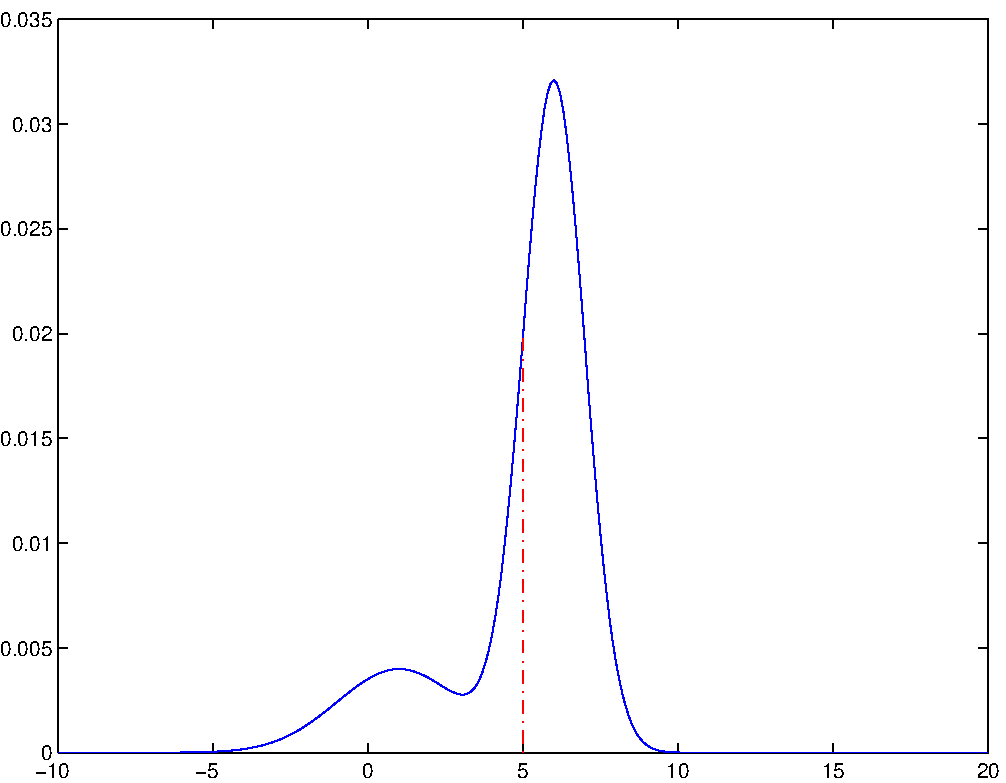
\includegraphics[width=.9\linewidth]{figure}
%\caption{\tiny{Distribution $f(x)$: $\mathbb{E}_{f}(x)=5$.}}
\end{center}
\end{figure}
\end{columns}
\end{exampleblock}
}
%%%%%%%%%%%%%%%%%%%%%%%%%%%%%%%%%%%%%%%%%%%%%%%%%%%%%%%%%%%%%
\frame
{
\frametitle{Estimating the mean knowing the observations $\mathbf{x}$}

\begin{exampleblock}{Example A}
\begin{columns}
\column[t]{.5\linewidth}
Observations $\mathbf{x}=(x_1,\cdots,x_{100})$ :
\tiny
$$
\left\lbrace
\begin{array}{ccccc}
   7.0411 &  4.8397 &  5.3156 &  6.7719 &  7.0616 \\
    5.2546 &   7.3937 &  4.3376 &   4.4010&    5.1724\\
    7.4199 &   5.3677 &  6.7028 &   6.2003 &   7.5707\\
    4.1230 &   3.8914 &   5.2323 &  5.5942 &    7.1479\\
  3.6790 &     0.3509 &   1.4197&   1.7585 &   2.4476\\
   -3.8635 &   2.5731 &   -0.7367 &  0.5627 &   1.6379\\
   -0.1864 &   2.7004 &   2.1487 &  2.3513 &   1.4833\\
   -1.0138 &  4.9794 &  0.1518 &  2.8683 &  1.6269 \\
    6.9523 & 5.3073 &  4.7191 &   5.4374 &   4.6108 \\
    6.5975 &  6.3495 & 7.2762 &  5.9453 &   4.6993\\
    6.1559&  5.8950 &  5.7591 &  5.2173 &   4.9980\\
    4.5010 &  4.7860 &  5.4382 &   4.8893&  7.2940\\
    5.5741 &  5.5139 &  5.8869 &  7.2756 &   5.8449 \\
    6.6439 &  4.5224 &  5.5028 &  4.5672 &  5.8718 \\
    6.0919 &  7.1912 &  6.4181 &  7.2248 &  8.4153 \\
    7.3199 &  5.1305 &  6.8719 &  5.2686 &   5.8055 \\
    5.3602 &  6.4120 &  6.0721 &  5.2740 &  7.2329\\
    7.0912 &  7.0766 &  5.9750 &  6.6091 &  7.2135 \\
    4.9585 &  5.9042 &  5.9273 &  6.5762 &   5.3702\\
    4.7654 &  6.4668 &  6.1983 &  4.3450 &   5.3261\\
\end{array}\right\rbrace
$$
\column[t]{.5\linewidth}
\normalsize
From the samples, the mean can be computed:
$$
\begin{array}{ll}
\overline{x}&=\frac{\sum_{i=1}^{100}x_i}{100}\\
&\\
&=  4.9970\\
\end{array}
$$
\end{columns}
\end{exampleblock}
}


%%%%%%%%%%%%%%%%%%%%%%%%%%%%%%%%%%%%%%%%%%%%%%%%%%%%
\frame
{
\frametitle{Accuracy of arbituary estimates $\hat{\theta}$}


We can compute an estimate $\hat{\theta}$ of a parameter $\theta$ from an observation sample $\mathbf{x}=(x_1,x_2,\cdots,x_n)$. But 

\

\alert{how accurate is $\hat{\theta}$ compared to the real value $\theta$ ?}

\

Our attention is focused on questions concerning the probability distribution of $\hat{\theta}$. For instance we would like to know about:
\begin{itemize}
\item its standard error
\item its confidence interval
\item its bias
\item etc. 
\end{itemize}

}

%%%%%%%%%%%%%%%%%%%%%%%%%%%%%%%%%%%%%%%%%%%%
%%%%%%%%%%%%%%%%%%%%%%%%%%%%%%%%%%%%%%%%%%%%%



%%%%%%%%%%%%%%%%%%%%%%%%%%%%%%%%%%%%%%%%%%%%
\frame
{
\frametitle{Standard error of $\hat{\theta}$}
\begin{definition}
The \alert{standard error} is the standard deviation  of a statistic $\hat{\theta}$. As such, it measures the precision of an estimate of the statistic  of a population distribution.
$$
se(\hat{\theta})=\sqrt{var_{f}{[\hat{\theta}]}}
$$
\end{definition}

%\pause

\begin{exampleblock}{Standard error of  $\overline{x}$}
We have:
$$
\mathbb{E}_{f}\left\lbrack (\overline{x}-\mu_f)^2\right\rbrack=% \mathbb{E}_{f}\left\lbrack \left(\frac{\sum_{i=1}^n (x_i-\mu_{f})}{n}\right)^2\right\rbrack =
\frac{\sum_{i=1}^n \mathbb{E}_{f}\left\lbrack (x_i-\mu_{f})^2\right\rbrack}{n^2}=\frac{\sigma_{f}^{2}}{n}
$$
Then
$$
se_{f}(\overline{x})=\lbrack\mathrm{var}_{f}(\overline{x})\rbrack^{1/2}=\frac{\sigma_{f}}{\sqrt{n}}
$$

\end{exampleblock}
}


%%%%%%%%%%%%%%%%%%%%%%%%%%%%%%%%%%%%%%%%%%%%
\frame
{
\frametitle{Plug in estimate of the standard error}

Suppose now that $f$ is unknown and that only the random sample $\mathbf{x}=(x_1,\cdots,x_n)$ is known.
As $\mu_f$ and $\sigma_f$ are unknown, we can use the previous formula to compute a plug-in estimate of the  standard error.
\begin{definition}
The \alert{estimated standard error} of the estimator $\hat{\theta}$ is defined as:
$$
\hat{\mathrm{se}}(\hat{\theta})=\mathrm{se}_{\hat{f}}(\hat{\theta})=\lbrack\mathrm{var}_{\hat{f}}(\hat{\theta})\rbrack^{1/2}
$$
\end{definition}

%\pause

\begin{exampleblock}{Estimated standard error of $\overline{x}$ }
$$
\hat{\mathrm{se}} (\overline{x})=\frac{\hat{\sigma}}{\sqrt{n}}
$$
\end{exampleblock}
}

%%%%%%%%%%%%%%%
\frame
{
\frametitle{Example on the mouse data}

\begin{table}[!h]
\begin{tabular}{|c|c|}
\hline
&\\
 Data (Treatment group) & 94; 197; 16; 38; 99; 141; 23 \\
&\\
\hline
& \\
Data (Control group) & 52; 104; 146; 10; 51; 30; 40; 27; 46 \\
& \\
\hline
\end{tabular}
\caption{The mouse data [Efron]. 16 mice  assigned to a treatment group (7) or a control group (9). Survival in days following a test surgery.  }
\end{table}

\centering{\alert{\textbf{Did the treatment prolong survival ?}}}


}

\frame
{
\frametitle{Example on the mouse data}



\begin{exampleblock}{Mean and Standard error for both groups}
%Using the formulas, we have $\overline{x}_{Treat}=86.86$ and $\hat{\mathrm{se}}_{Treat}(\overline{x})=25.24$
%and $\overline{x}_{Cont}=56.22$ and $\hat{\mathrm{se}}_{Cont}(\overline{x})=14.14$. 
\begin{table}[!h]
\begin{tabular}{c|c|c}
& $\overline{x}$ & $\hat{\mathrm{se}} $ \\
\hline
Treatment & 86.86 & 25.24 \\
\hline
Control & 56.22 & 14.14 \\
\end{tabular}
\end{table}
\end{exampleblock}


\begin{block}{Conclusion at first glance} 
It seems that mice having the treatment survive $d=86.86-56.22=30.63$ days more than the mice from the control group.
\end{block}



}


\frame
{
\frametitle{Example on the mouse data}


\begin{exampleblock}{Stantard error of the difference $d=\overline{x}_{Treat}-\overline{x}_{Cont}$}
$\overline{x}_{Treat}$ and $\overline{x}_{Cont}$ are independent, so the standard error of their difference is $\hat{\mathrm{se}}(d)=\sqrt{\hat{\mathrm{se}}_{Treat}^2 +\hat{\mathrm{se}}_{Cont}^2 }=28.93$. 
We see that:
$$
\frac{d}{\hat{\mathrm{se}}(d)}
=\frac{30.63}{28.93}=1.05
 $$
This shows that this is an insignificant result as it could easily have arised by chance (i.e. if the test was reproduced, it is \textit{likely possible} to measure datasets giving $d=0$!).  

Therefore, we can not conclude with certainty that the treatment improves the survival of the mice.
\end{exampleblock}
}



%%%%%%%%%%%%%%%%%%%%%%%%%%%%%%%%%%%%%%%%%%%%
\frame
{
\frametitle{Confidence interval for $\hat{\theta}$}


\begin{definition}

Assuming that the estimator $\hat{\theta}$ is normally distributed with unknown expectation $\theta$ and variance $\mathrm{se}^2$, then :

$$
\mathrm{Prob}\lbrace \hat{\theta}-z^{(1-\alpha)} \mathrm{se}\leq  \theta \leq \hat{\theta}- z^{(\alpha)} \mathrm{se}\rbrace=1-2\alpha
$$
Therefore   $1-2\alpha$ \% \alert{confidence interval} for $\theta$ is
$
\lbrack \hat{\theta}-z^{(1-\alpha)}\mathrm{se} ; \hat{\theta}- z^{(\alpha)} \mathrm{se}\rbrack
$

\alert{Confidence limits} are the lower and upper boundaries  values of a confidence interval. The \alert{confidence level} is the probability value $100 \times (1-2\alpha)$ \% associated with a confidence interval.

\end{definition}


}
%%%%%%%%%%%%%%%%%%%%%%%%%%%%%%%%%%%%%%%%%%%%%
\frame
{
\frametitle{Confidence interval}

The width of the confidence interval gives us some idea about how uncertain we are about the unknown parameter. A very wide interval may indicate that more data should be collected before anything very definite can be said about the parameter.

\begin{columns}
\column[t]{0.5\linewidth}
\begin{table}[!h]
\begin{tabular}{|c|c|c|}
\hline
\tiny{percentile} &\tiny{confidence level}& \\
$\alpha\times 100$ \% & $(1-2\alpha)\times 100$  \% & $z^{(1-\alpha)}$\\
\hline
10 &80 & $1.28155 $ \\	
5 & 90 &	$1.64485$ \\
2.5 & 95 	& $1.95996 $ \\
0.5 & 99 	& $2.57583 $ \\
0.25 &99.5 	& $2.80703 $ \\
0.05 &99.9 	& $3.29053 $ \\
\hline
\end{tabular}
\caption{\tiny{For a normal p.d.f $z^{(\alpha)}=-z^{(1-\alpha)}$}}
\end{table}
\column[t]{0.5\linewidth}
\begin{figure}[!h]
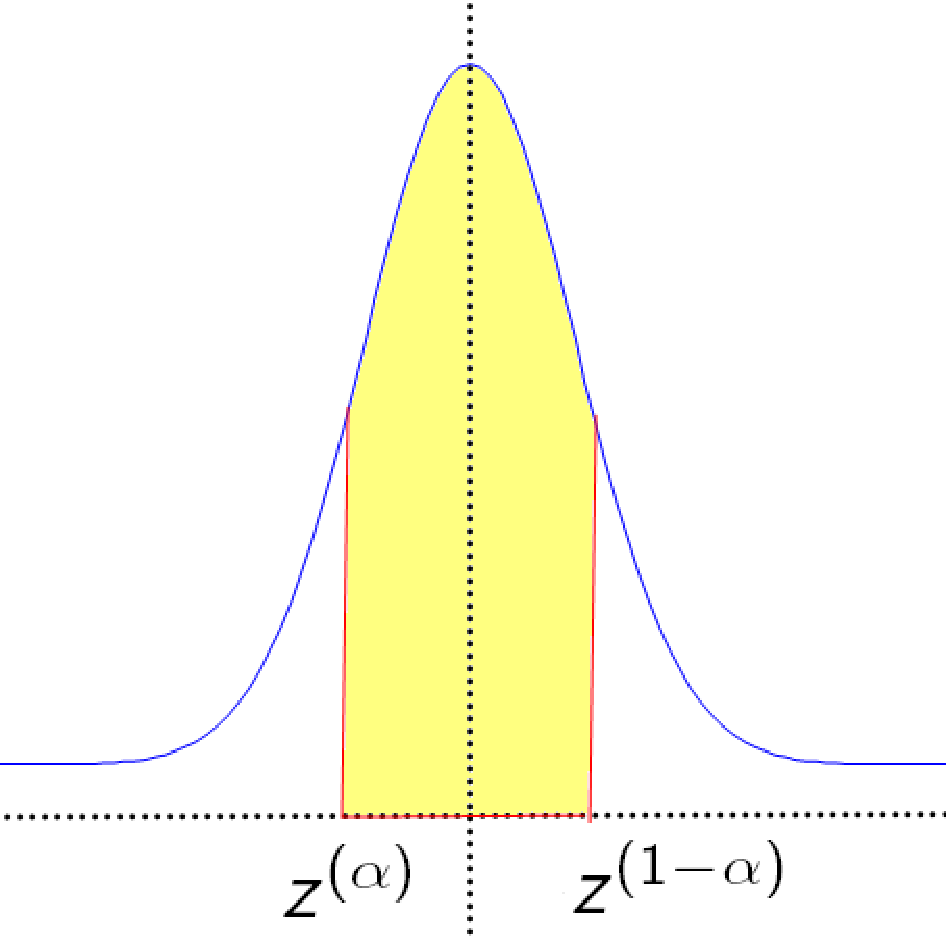
\includegraphics[width=.6\linewidth]{gaussien.pdf}
\caption{ \tiny{Density function $\mathcal{N}(0,1)$.}}
\end{figure}
\end{columns}
}
%%%%%%%%%%%%%%%%%%%%%%%%%%%%%%%%%%%%%%%%%%
\frame
{
\frametitle{Example Confidence interval}

\begin{exampleblock}{Confidence interval of the mean}
Using the central limit theorem, the estimate  $\overline{x}$ is following a normal density function $\mathcal{N}\left(\mu_f,\frac{\sigma_f^2}{n}\right)$.
The 90\% confidence interval is :
$$
\overline{x}\pm 1.645 \frac{\sigma_f}{\sqrt{n}}\  \mathrm{estimated\ by} \pm 1.645 \frac{\hat{\sigma}}{\sqrt{n}}
$$
\end{exampleblock}

\begin{exampleblock}{confidence interval of the difference for the mouse data}
The difference $d$ in days of survival between the treatment group and the control group has a estimated 90\% confidence interval defined as:
$$
 d=30.63\pm  1.645\times 28.93=30.63 \pm 47.5898 
$$
\end{exampleblock}
}
%%%%%%%%%%%%%%%%%%%%%%%%%%%%%%%%%%%%%%%%%%
\frame
{
\frametitle{Bias of $\hat{\theta}$}
\begin{definition}
The \alert{Bias} is the difference between the expectation of an estimator $\hat{\theta}$ and the quantity $\theta$ being estimated:
$$
\mathrm{Bias}_{f}(\hat{\theta},\theta)=\mathbb{E}_f(\hat{\theta})-\theta
$$
\end{definition}


 \begin{exampleblock}{Bias of the mean $\overline{x}$}
we have:
$$
\mathbb{E}_{f}(\overline{x})=\mathbb{E}_{f}\left(\frac{\sum_{i=1}^{n} x_i}{n}\right)=\frac{\sum_{i=1}^{n}\mathbb{E}_{f}( x_i)}{n}=\mu_f
$$
then:
$$
\mathrm{Bias}_{f}(\overline{x},\mu_f)=\mathbb{E}_f(\overline{x})-\mu_f =0
$$
\end{exampleblock}
}

%% lots of mistakes -
\frame
{
\frametitle{Bias of $\hat{\theta}$}

\begin{itemize}
\item A large bias is usually an undesirable aspect of an estimator's performance. \alert{Unbiased estimates} (such $\mathbb{E}_f(\hat{\theta})=\theta$) are interesting in practice as they promote a nice feeling of scientific objectivity in the estimation process. 
%\item Plug- in estimates $\hat{\theta}=t(\hat{f})$ are not necessarily unbiased but they tend to have small biases compared to the magnitude of their standard error.
\end{itemize}

\begin{exampleblock}{Bias of $\hat{\sigma}^2$}
$$
\begin{array}{ll}
\hat{\sigma}^2&=\frac{1}{n} \sum_{i=1}^{n} (x_i-\overline{x})^{2}=\frac{1}{n} \sum_{i=1}^{n} ((x_i-\mu_f)+ (\mu_f-\overline{x}))^{2}\\
&\\
&=\left(\frac{1}{n}  \sum_{i=1}^{n} (x_i-\mu_f)^2 \right)-  (\overline{x}-\mu_f)^2\\
\end{array}
$$
The first term has an expected value of $\sigma_f^2$ and the second term has expected value $\sigma_f^2/n$. So the bias of  $\hat{\sigma}^2$ is:
$$
\mathrm{Bias}_{f}(\hat{\sigma}^2,\sigma_f^2)=\sigma_f^2-\frac{\sigma_f^2}{n}-\sigma_f^2=-\frac{\sigma_f^2}{n}
$$ 
\end{exampleblock}
}

%% lots of mistakes -
\frame
{
\frametitle{Bias of $\hat{\theta}$}

Instead of using $\hat{\sigma}^2$ as an estimate of the variance, you should try to choose an unbiased estimate. 

\begin{exampleblock}{Bias of $\overline{\sigma}^2$}
Let define:
$$ 
\overline{\sigma}^2=\frac{1}{n-1} \sum_{i=1}^{n} (x_i-\overline{x})^{2}
$$
then by computing its bias:
$$
\begin{array}{ll}
\mathrm{Bias}_f(\overline{\sigma}^2,\sigma_f^2)&=\mathbb{E}_{f}(\overline{\sigma}^2)-\sigma_f^2\\
&=0\\
\end{array}
$$
$\overline{\sigma}$ is an unbiased estimator of the standard deviation.
\end{exampleblock}


}

%%%%%%%%%%%%%%%%%%%%%%%%%%%%%%%%%%%%%%%%%%
\frame{
\frametitle{Summary }


\begin{itemize}
\item Population density function $f(\cdot)$ and empirical density function $\hat{f}(\cdot)$, 

\

\item Plug-in principle: relation between $\theta$ and its estimate $\hat{\theta}$ 

\

\item Standard error and confidence interval as a measure of accuracy of the estimate $\hat{\theta}$ 

\

\item Accuracy of estimate is important to draw conclusions (e.g. mouse example). 

\

\item se has an explicit expression for the mean $\overline{x}$
\end{itemize}

}

\frame{
\frametitle{Open problems}

\begin{itemize}
\item $f$ is generally unknown! 

\

\item Using the Plug-in principle, with more samples $\lbrace \mathbf{x} \rbrace$ drawn from $f$, we could estimate $\hat{se}$ or the bias.

\

\item But the only information available is one sample $\mathbf{x}=(x_1, \cdot,x_n)$ drawn from $f$! 

\

\item Most of all, explicit expression of $\mathrm{se}$ of the estimate is not easy to get in most cases!

\end{itemize}

}


%%%%%%%%%%%%%%%%%%%%%%%%%
\section{Non-Parametric Bootstrap}
\frame{
\frametitle{Introduction to resampling methods}
\begin{itemize}
\item Definitions and Problems
\item \textbf{Non-Parametric Bootstrap}
\item Parametric Bootstrap
\item Jackknife
\item Permutation tests
\item Cross-validation
\end{itemize}
}
\frame
{
\frametitle{Introduction}


 We want to assess the accuracy (bias, standard error, etc.) of an arbitrary estimate $\hat{\theta}$ knowing only one sample $\mathbf{x}=(x_1,\cdots,x_n)$ drawn from an unknown population  density function $f$.

\begin{itemize}
\item We propose here one way, called \textit{Bootstrap}, to do it using computer intensive techniques for resampling. 

\

\item Bootstrap is a data based simulation method for statistical inference. The basic idea of bootstrap is to use the sample data to compute a statistic and to estimate its sampling distribution, without any model assumption. 

\

\item No theoretical calculations of standard errors needed so we don't care how mathematically  complex the estimator $\hat{\theta}$ can be! 

 \end{itemize}



}

\frame
{
\frametitle{Introduction}


\begin{itemize}
\item The (non-parametric) bootstrap method is an application of the plug-in principle.   By \textit{non-parametric}, we mean that only $\mathbf{x}$ is known (observed) and no prior knowledge on the population density function $f$ is available.

\

\item Originally, the Bootstrap was introduced to compute standard error of an arbitrary estimator by  Efron (1979) and to-date the basic idea remains the same.
\

\item The term \alert{bootstrap} derives from the phrase \textit{to pull oneself up by one's bootstrap} (Adventures of Baron Munchausen, by Rudolph Erich Raspe). The Baron had fallen to the bottom of a deep lake. Just when it
looked like all was lost, he thought to pick himself up by his own
bootstraps.

%\item It is not the same as the term .bootstrap. used in computer science to .boot. a computer from a set of core instructions (though the derivation is similar).
\end{itemize}


}

%%%%%%%%%%%%%%%%%%%%%%%%%%%%%%%%%%%%%%%%%%%%%%%%%%%%%%%%


\frame
{
\frametitle{Bootstrap samples and replications}

\begin{definition}
A \alert{bootstrap sample} $\mathbf{x}^{*}=(x^{*}_{1},x^{*}_{2},\cdots,x^{*}_{n})$ is obtained by randomly sampling $n$ times, with replacement, from the original data points $\mathbf{x}=(x_{1},x_{2},\cdots,x_{n})$.
\end{definition}

\begin{exampleblock}{}
Considering a sample $\mathbf{x}=(x_1,x_2,x_3,x_4,x_5)$, some bootstrap samples can be: 
$$
\begin{array}{l}
\mathbf{x}^{*(1)}=( x_{2},x_{3},x_{5},x_{4},x_{5})\\
\mathbf{x}^{*(2)}=( x_{1},x_{3},x_{1},x_{4},x_{5})\\
\mathrm{etc.}\\
\end{array}
$$
\end{exampleblock}
\begin{definition}
With each bootstrap sample $\mathbf{x}^{*(1)}$ to  $\mathbf{x}^{*(B)}$, we can compute a \alert{bootstrap replication} $\hat{\theta}^{*}(b)=s(\mathbf{x}^{*(b)})$ using the plug-in principle. 
\end{definition}

}
%%%%%%%%%%%%%%%%%%%%%%%%%%%%%%%%%%%%%%%%%%%%%
\frame
{
\frametitle{How to compute Bootstrap samples}

\begin{block}{}
Repeat $B$ times: 
\begin{enumerate}
\item A random number device selects integers $i_1,\cdots, i_n$ each of which equals any value between 1 and $n$ with probability $\frac{1}{n}$.
\item Then compute $\mathbf{x}^{*}=(x_{i_1},\cdots,x_{i_n})$.
\end{enumerate}
\end{block}

\begin{exampleblock}{Some matlab code available on the web}
See BOOTSTRAP MATLAB TOOLBOX, by Abdelhak M. Zoubir and D. Robert Iskander, 
 
\href{http://www.csp.curtin.edu.au/downloads/bootstrap_toolbox.html}{http://www.csp.curtin.edu.au/downloads/bootstrap\_toolbox.html}
\end{exampleblock}


}
%%%%%%%%%%%%%%%%%%%%%%%%%%%%%%%%%%%%%%%%%%%%%%%%%%%%%%
\frame{
\frametitle{How many values are left out of a bootstrap resample ?}
Given a sample $\mathbf{x}=(x_1,x_2,\cdots,x_n)$ and assuming that all $x_i$ are different, the probability that a particular value $x_i$ is left out of a resample $\mathbf{x}^{*}=(x_1^{*},x_2^{*},\cdots,x_n^{*})$ is:
$$
\mathcal{P}(x_{j}^{*}\neq x_i, 1\leq j \leq n)=\left(1-\frac{1}{n}\right)^n
$$
since $\mathcal{P}(x_{j}^{*}=x_i)=\frac{1}{n}$. 
 When $n$ is large, the probability  $\left(1-\frac{1}{n}\right)^n$  converges to $e^{-1}\approx 0.37$. 

%It also means that the expected proportion of values $x_i$s that are not represented in a particular resample $\mathbf{x}^{*}$ is  $\left(1-\frac{1}{n}\right)^n$.

} 
%%%%%%%%%%%%%%%%%%%%%%%%%%%%%%%%%%%%%%%%%%%%%%%%%%%%%%
%\frame{
%\frametitle{Bootstrap replications}
%\begin{definition}
%With each bootstrap sample $\mathbf{x}^{*(1)}$ to  $\mathbf{x}^{*(B)}$, we can compute a \alert{bootstrap replication} $\hat{\theta}^{*}(b)=s(\mathbf{x}^{*(b)})$ using the plug-in principle. 
%\end{definition}

%\begin{exampleblock}{What is the probability that  $\hat{\theta}^{*}(b)=\hat{\theta}$ ?}
%From the previous slide, the probability of that a bootstrap replication is identical to the estimate $\hat{\theta}$ is:
%$$
%\mathcal{P}(\hat{\theta}^{*}(b)=\theta)=1-\left(1-\frac{1}{n}\right)^n
%$$
%When $n$ large, $\mathcal{P}(\hat{\theta}^{*}(b)=\theta)=0.632$
%\end{exampleblock}
%}

%%%%%%%%%%%%%%%%%%%%%%%%%%%%%%%%%%%%%%%%%%%%%%%%%%%%%%
\frame{
\frametitle{The Bootstrap algorithm for Estimating standard errors}

\begin{beamercolorbox}[wd=\linewidth, rounded=true,shadow=true]{postit}
\begin{enumerate}
\item Select $B$ independent bootstrap samples $\mathbf{x}^{*(1)}, \mathbf{x}^{*(2)}, \cdots, \mathbf{x}^{*(B)}$ drawn from $\mathbf{x}$ 
\item Evaluate the bootstrap replications:
$$ 
\hat{\theta}^{*}(b)=s(\mathbf{x}^{*(b)}), \quad \forall b \in \lbrace 1,\cdots,B \rbrace
$$

\item Estimate the standard error $\mathrm{se}_{f}(\hat{\theta})$ by the standard deviation of the $B$ replications:
$$ 
\hat{\mathrm{se}}_{B}=\left\lbrack \frac{\sum_{b=1}^{B}\lbrack \hat{\theta}^{*}(b)-\hat{\theta}^{*}(\cdot)\rbrack^{2}}{B-1} \right\rbrack^{\frac{1}{2}}
$$
where $\hat{\theta}^{*}(\cdot)=\frac{\sum_{b=1}^{B} \hat{\theta}^{*}(b)}{B}$
\end{enumerate}
\end{beamercolorbox}
}
%%%%%%%%%%%%%%%%%%%%%%%%%%%%%%%%%%%%%%%%%%%%%%%%%%%%%
\frame{
\frametitle{Bootstrap  estimate of the standard Error}
\begin{exampleblock}{Example A}
From the distribution  $f$: $f(x)=0.2\ \mathcal{N}(\scriptstyle \mu=1,\sigma=2 \displaystyle) +0.8\  \mathcal{N}( \scriptstyle\mu=6,\sigma=1 \displaystyle)
$. We draw the sample  $\mathbf{x}=(x_1,\cdots,x_{100})$ :
\tiny
$$
\mathbf{x}=
\left\lbrace
\begin{array}{ccccc}
   7.0411 &  4.8397 &  5.3156 &  6.7719 &  7.0616 \\
    5.2546 &   7.3937 &  4.3376 &   4.4010&    5.1724\\
    7.4199 &   5.3677 &  6.7028 &   6.2003 &   7.5707\\
    4.1230 &   3.8914 &   5.2323 &  5.5942 &    7.1479\\
  3.6790 &     0.3509 &   1.4197&   1.7585 &   2.4476\\
   -3.8635 &   2.5731 &   -0.7367 &  0.5627 &   1.6379\\
   -0.1864 &   2.7004 &   2.1487 &  2.3513 &   1.4833\\
   -1.0138 &  4.9794 &  0.1518 &  2.8683 &  1.6269 \\
    6.9523 & 5.3073 &  4.7191 &   5.4374 &   4.6108 \\
    6.5975 &  6.3495 & 7.2762 &  5.9453 &   4.6993\\
    6.1559&  5.8950 &  5.7591 &  5.2173 &   4.9980\\
    4.5010 &  4.7860 &  5.4382 &   4.8893&  7.2940\\
    5.5741 &  5.5139 &  5.8869 &  7.2756 &   5.8449 \\
    6.6439 &  4.5224 &  5.5028 &  4.5672 &  5.8718 \\
    6.0919 &  7.1912 &  6.4181 &  7.2248 &  8.4153 \\
    7.3199 &  5.1305 &  6.8719 &  5.2686 &   5.8055 \\
    5.3602 &  6.4120 &  6.0721 &  5.2740 &  7.2329\\
    7.0912 &  7.0766 &  5.9750 &  6.6091 &  7.2135 \\
    4.9585 &  5.9042 &  5.9273 &  6.5762 &   5.3702\\
    4.7654 &  6.4668 &  6.1983 &  4.3450 &   5.3261\\
\end{array}\right\rbrace
$$
\normalsize
We have $\mu_f=5$ and $\overline{x}=4.9970$.

\end{exampleblock}
}
%%%%%%%%%%%%%%%%%%%%%%%%%%%%%%%%%%%%%%%%%%%%%%%%%%%%%
\frame{
\frametitle{Bootstrap  estimate of the standard Error}

\begin{exampleblock}{Example A}
\begin{enumerate}
\item $B=1000$ bootstrap samples $\lbrace \mathbf{x}^{*(b)}\rbrace $
\item $B=1000$ replications $\lbrace\overline{x}^{*}(b)\rbrace$
\item Bootstrap estimate of the standard error:
$$
\widehat{\mathrm{se}}_{B=1000}=\left\lbrack \frac{\sum_{b=1}^{1000}\lbrack \overline{x}^{*}(b)-\overline{x}^{*}(\cdot)\rbrack^{2}}{1000-1} \right\rbrack^{\frac{1}{2}}=0.2212
$$
where $\overline{x}^{*}(\cdot)=5.0007$.
This is to compare with $\hat{se}(\overline{x})=\frac{\hat{\sigma}}{\sqrt{n}}=0.22$.

\end{enumerate}

\end{exampleblock}
}
%%%%%%%%%%%%%%%%%%%%%%%%%%%%%%%%%%%%%%%%%%%%%%%%%%%%%%%%
\frame
{
\frametitle{Distribution of $\hat{\theta}$}

\begin{block}{}
When enough bootstrap resamples have been generated, not only the standard error but any aspect of the distribution  of the estimator $\hat{\theta}=t(\hat{f})$ could be estimated. One can draw a histogram of the distribution of  $\hat{\theta}$ by using the observed $\hat{\theta}^{*}(b),\ b=1,\cdots,B $. 
\end{block}

\begin{exampleblock}{Example A}

\begin{figure}[!h]
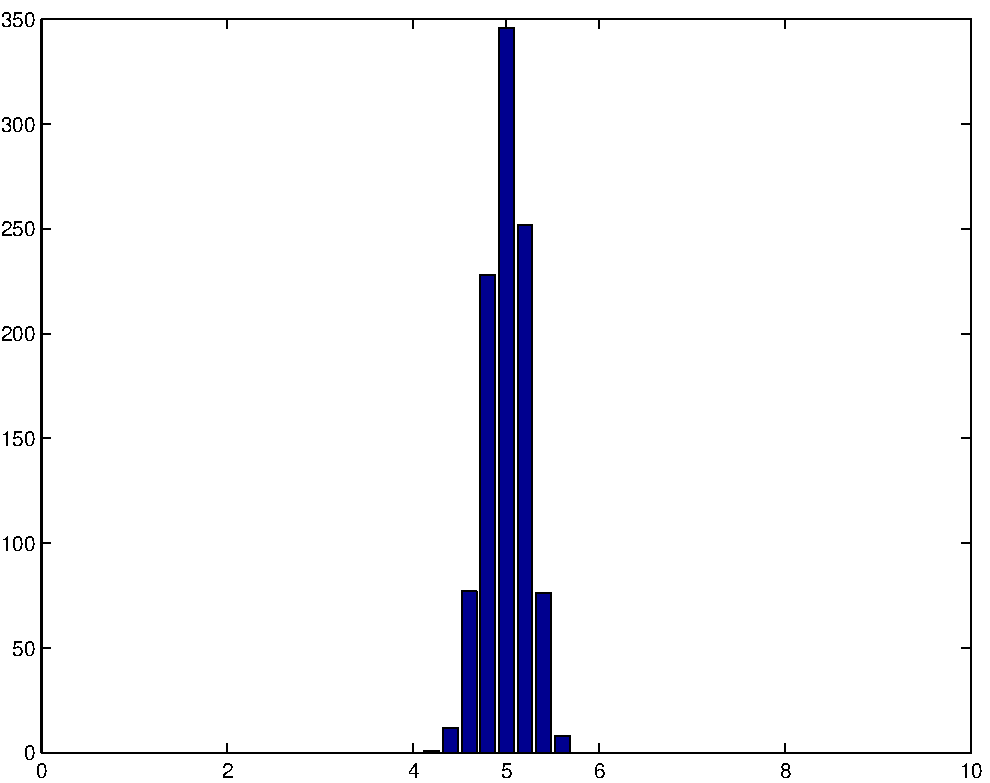
\includegraphics[width=.4\linewidth]{histoExampleA.pdf}
\caption{\small Histogram of the replications $\lbrace\overline{x}^{*}(b)\rbrace_{b=1\cdots B}$. }
\end{figure}
\end{exampleblock}

}
%%%%%%%%%%%%%%%%%%%%%%%%%%%%%%%%%%%%%%%%%%%%%%%%%%%%%%%%%%%%%%
\frame
{
\frametitle{Bootstrap estimate of the standard error}

\begin{definition}
The ideal bootstrap estimate $\mathrm{se}_{\hat{f}} (\hat{\theta}^{*})$ is defined as:
$$
\lim_{B\rightarrow \infty} \hat{\mathrm{se}}_{B}=\mathrm{se}_{\hat{f}} (\hat{\theta}^{*})
$$
 $\mathrm{se}_{\hat{f}} (\hat{\theta}^{*})$ is called a \alert{non-parametric bootstrap estimate of the standard error}.
%When $n$ and $B$ large, the hope is that $\hat{\mathrm{se}}_{B}$ will be close to $\mathrm{se}_{\hat{F}} (\theta^{*})$ which will be close to $\mathrm{se}_{F}(\theta)$.
\end{definition}
}

%%%%%%%%%%%%%%%%%%%%%%%%%%%%%%%%%%%%%%%%%%%%%%%%%%%%%5
\frame{
\frametitle{Bootstrap  estimate of the  standard Error}

\begin{block}{How many $B$ in practice ?}
you may want to limit the computation time.
In practice, you get a good estimation of the standard error for $B$ in between 50 and 200.  
\end{block}
\begin{exampleblock}{Example A}
\begin{table}[!h]
\begin{tabular}{|c|c|c|c|c|c|c|c|}
\hline
$B$& 10& 20 & 50 & 100 & 500 & 1000  & 10000\\
\hline
$\widehat{\mathrm{se}}_{B}$& 0.1386 & 0.2188 & 0.2245 & 0.2142 & 0.2248& 0.2212 & 0.2187\\
\hline
\end{tabular}
\caption{Bootstrap standard error w.r.t. the number $B$ of bootstrap samples.}
\end{table}

\end{exampleblock}
}



%%%%%%%%%%%%%%%%%%%%%%%%%%%%%%%%%%%%%%%%%%%%%%%%%%%%%%%%%%%%%%
\frame{
\frametitle{Bootstrap estimate of bias}
\begin{definition}
The \alert{bootstrap estimate of bias} is defined to be the estimate:
 $$
\begin{array}{ll}
\mathrm{Bias}_{\hat{f}}(\hat{\theta})&=\mathbb{E}_{\hat{f}}\lbrack s(\mathbf{x}^{*})\rbrack-t(\hat{f})\\
&\\
&= \hat{\theta}^{*}(\cdot)-\hat{\theta}
\end{array}
$$
%Here $t(\hat{F})$ may differ from the plug-in estimate $\hat{\theta}$ i.e. $\mathrm{Bias}_{\hat{F}}$ is the plug-in estimate of $\mathrm{Bias}_{F}$ whether or not $\hat{\theta}$ is the plug-in estimate of $\theta$.
\end{definition}

\begin{exampleblock}{Example A}

\small
\begin{table}[!h]
\begin{tabular}{|l|c|c|c|c|c|c|c|}
\hline
B & 10 & 20 & 50 & 100 & 500 & 1000 & 10000 \\
\hline
$\mathbb{E}_{\hat{f}}(\overline{x}^{*})$ & 5.0587 & 4.9551 &5.0244 & 4.9883 &  4.9945 & 5.0035 & 4.9996 \\
\hline
$\widehat{\mathrm{Bias}}$ & 0.0617 & -0.0419 & 0.0274 & -0.0087 & -0.0025 &  0.0064 &0.0025 \\
\hline
\end{tabular}
\caption{$\widehat{\mathrm{Bias}}$ of  $\overline{x}^{*}$ ($\overline{x}=4.997$ and $\mu_f=5$). }
\end{table}
\end{exampleblock}
}
%%%%%%%%%%%%%%%%%%%%%%%%%%%%%%%%%%%%%%%%%%%%%%%%%%%%%%%%%%%%%%
\frame{
\frametitle{Bootstrap estimate of bias}
\begin{beamercolorbox}[wd=\linewidth, rounded=true,shadow=true]{postit}
\begin{enumerate}
\item $B$ independent bootstrap samples $\mathbf{x}^{*(1)}, \mathbf{x}^{*(2)}, \cdots, \mathbf{x}^{*(B)}$ drawn from $\mathbf{x}$ 
\item Evaluate the bootstrap replications:
$$ 
\hat{\theta}^{*}(b)=s(\mathbf{x}^{*(b)}), \quad \forall b \in \lbrace 1,\cdots,B \rbrace
$$
\item Approximate the bootstrap expectation :
$$
\hat{\theta}^{*}(\cdot)=\frac{1}{B} \sum_{b=1}^{B} \hat{\theta}^{*}(b)=\frac{1}{B} \sum_{b=1}^{B} s(\mathbf{x}^{*(b)})
$$
\item the bootstrap estimate of bias based on $B$ replications is:
$$
\widehat{\mathrm{Bias}}_{B}=\hat{\theta}^{*}(\cdot)-\hat{\theta}
$$
\end{enumerate}
\end{beamercolorbox}
}
%%%%%%%%%%%%%%%%%%%%%%%%%%%%%%%%%%%%%%%%%%%%%%%%%%%%%%%%%%%%%
\frame{
\frametitle{Confidence interval}

\begin{definition}
Using the bootstrap estimation of the standard error, the $100(1-2\alpha)$\%
confidence interval is:
$$
\theta=\hat{\theta} \pm z^{(1-\alpha)} \cdot \widehat{\mathrm{se}}_{B}
$$
\end{definition}

\begin{definition}
If the bias in not null,  the \alert{bias corrected 
confidence interval} is defined by:
$$
\theta=(\hat{\theta}-\widehat{\mathrm{Bias}}_{B}) \pm z^{(1-\alpha)} \cdot \widehat{\mathrm{se}}_{B}
$$
\end{definition}
} 

%%%%%%%%%%%%%%%%%%%%%%%%%%%%%%%%%%%%%%%%%%%%%%%%%%%%%%%%%%%%%%
\frame{
\frametitle{Can the bootstrap answer other questions?}
\begin{exampleblock}{The mouse data}


\begin{table}[!h]
\begin{tabular}{|c|c|}
\hline
&\\
 Data (Treatment group) & 94; 197; 16; 38; 99; 141; 23 \\
&\\
\hline
& \\
Data (Control group) & 52; 104; 146; 10; 51; 30; 40; 27; 46 \\
& \\
\hline
\end{tabular}
\caption{The mouse data [Efron]. 16 mice divided assigned to a treatment group (7) or a control group (9). Survival in days following a test surgery. \alert{Did the treatment prolong survival ?} }
\end{table}


\end{exampleblock}
}
%%%%%%%%%%%%%%%%%%%%%%%%%%%%%%%%%%%%%%%%%%%%%%%%%%%%%%%%%%%%%%
\frame{
\frametitle{Can the bootstrap answer other questions?}
\begin{exampleblock}{The mouse data}
%
\begin{table}[!h]
\begin{tabular}{ccccccc}
$B$ &  50   &  100 & 250   & 500 & 1000 & $\infty$ \\
\hline
$\hat{\mathrm{se}}_{B} (\overline{x}_{Treat})$  & 19.72 & 23.63 & 22.32 & 23.79 & 23.02 & 23.36 \\
%median & 32.21 & 36.35 & 34.46 & 36.72 & 36.48 & 37.83 \\
$\hat{\mathrm{se}}_{B} (\overline{x}_{Cont})$  & - & 11.54 & - & - & - & 9.73 \\
 \end{tabular}
\caption{Bootstrap estimates of the standard error for the mean  for the treatment and control groups of the mouse data.}
\end{table} 

\textbf{Standard error of the difference for $B=100$ Bootstrap replications.}
The observed difference is $d^{*}=48$ with an estimated standard error of $\widehat{\mathrm{se}}_{100}(d^*)=38.14$.
The ratio $48/38.14=1.26$ is better (than $d/\mathrm{se}(d)=1.05$ cf.1st lecture) but still insignificant. 




\begin{itemize}

\item Remember in the first lecture, we compute $d=\overline{x}_{Treat}-\overline{x}_{Cont}=30.63$ with a standard error $\hat{se}(d)=28.93$. The ratio was $d/\hat{se}(d)=1.05$ (an insignificant result as measuring $d=0$ is likely possible).

\item Using bootstrap method
\begin{enumerate}
\item  $B$ bootstrap samples $\mathbf{x}_{Treat}^{*(b)}=(x_{Treat\ 1}^{*(b)},\cdots,x_{Treat\ 7}^{*(b)})$ and $\mathbf{x}_{Cont}^{*(b)}=(x_{Cont\ 1}^{*(b)},\cdots,x_{Cont\ 9}^{*(b)})$, $\forall 1\leq b \leq B$

\item $B$ bootstrap replications are computed: $d^{*}(b)=\overline{x}^{*(b)}_{Treat}-\overline{x}^{*(b)}_{Cont}$

\item  The bootstrap  standard error is computed for $B=1400$: $\hat{se}_{B=1400}=26.85$.  
\item The ratio is  $d/\hat{se}_{1400}(d)=1.14$.
\end{enumerate}
\item This is still not a significant result. 
\end{itemize}

\end{exampleblock}
}
%%%%%%%%%%%%%%%%%%%%%%%%%%%%%%%%%%%%%%%%%%%%%%%%%%%%%%%%%%%%%%
%%%%%%%%%%%%%%%%%%%%%%%%%%%%%%%%%%%%%%%%%%%%%%%%%%%%%%%%%%%%%%
\frame
{
\frametitle{The Law school example}

%\small
\begin{table}[!h]
\begin{flushleft}
\begin{tabular}{lcccccccc}
School &   1  &   2 &    3   &  4  &   5  &   6   &  7  &   8  \\
\hline
LSAT (X) & 576  &  635  &  558 &   578  &  666  &  580  &  555   & 661  \\
GPA (Y) &  3.39   &  3.30   &  2.81   &  3.03  &   3.44   &  3.07   &  3.00   &  3.43 \\

&&&&&&&&\\
\end{tabular}

\begin{tabular}{lccccccc}

School &       9   & 10   & 11 &   12  &  13  &  14   & 15 \\
\hline
LSAT (X) &  651   & 605  &  653  &  575   & 545  &  572  &  594 \\
GPA (Y) &    3.36   &  3.13  &   3.12  & 2.74   &  2.76   &  2.88   &  2.96\\

\end{tabular}
\end{flushleft}
\caption{Results of law schools admission practice  for the LSAT and GPA tests. It is believed that these scores are highly correlated. \alert{Compute the correlation and its standard error.}}
\end{table}


}



\frame
{
\frametitle{Correlation}
The correlation is defined :
$$ 
\mathrm{corr}(X,Y)=\frac{\mathbb{E}\lbrack (X -\mathbb{E}(X)) \cdot (Y -\mathbb{E}(Y))\rbrack }{\left( \mathbb{E} \lbrack (X -\mathbb{E}(X))^2 \rbrack  \cdot \mathbb{E} \lbrack (Y -\mathbb{E}(Y))^2 \rbrack \right)^{1/2}}
$$ 

Its typical estimator is:
$$
\widehat{\mathrm{corr}}(\mathbf{x},\mathbf{y})=\frac{\sum_{i=1}^{n} x_i\ y_i - n\ \overline{x}\ \overline{y}}{\lbrack \sum_{i=1}^{n}x_i^2-n\overline{x}^2 \rbrack^{1/2}\cdot \lbrack\sum_{i=1}^{n} y_i^2-n \overline{y}^2 \rbrack^{1/2} }
$$

}


\frame{
\frametitle{The Law school example}
\begin{itemize}
\item The estimated correlation is $\widehat{\mathrm{corr}}(\mathbf{x},\mathbf{y})=.7764$ between LSAT and GPA. 
%\item Precise theoretical formula for the standard error of the estimator is unavailable.
\end{itemize}
\begin{exampleblock}{Non-parametric Bootstrap estimate of the standard error}

\begin{table}[!h]
\begin{tabular}{l|cccccccc}
$B$ & 25 & 50 & 100 & 200 & 400 & 800 & 1600 & 3200 \\
\hline
$\hat{\mathrm{se}}_B$& .140 & .142 & .151 & .143 & .141 &.137 & .133 & .132 \\
\end{tabular}
\caption{Bootstrap estimate of standard error for $\widehat{\mathrm{corr}}(\mathbf{x},\mathbf{y})=.776$.}
\end{table}
The standard error stabilizes to $\mathrm{se}_{\hat{f}} (\widehat{\mathrm{corr}})\approx.132$.  
\end{exampleblock}
}

%%%%%%%%%%%%%%%%%%%%%%%%%%%%%%%%%%%%%%%%%%%%%%%%%%%%%%%
\frame{
\frametitle{The Law school example: Conclusion}

\begin{itemize}
\item The textbook formula for  the correlation coefficient is:
 $$
\hat{\mathrm{se}}(\widehat{\mathrm{corr}})=(1-\widehat{\mathrm{corr}}^2)/\sqrt{n-3}
$$
\item With $\widehat{\mathrm{corr}}=0.7764$, the standard error is $\hat{se}(\widehat{\mathrm{corr}})=0.1147$.
\item The estimated non-parametric bootstrap  standard error $\mathrm{se}_{B=3200}$ is $0.132$.
%\item The parametric bootstrap  standard error for $B=3200$ is $0.1169$.
\end{itemize}

}
%%%%%%%%%%%%%%%%%%%%%%%%%%%%%%%%%%%%%%%%%%%%%%%%%%%%%%%%
%%%%%%%%%%%%%%%%%%%%%%%%%%%%%%%%%%%%%%%%%%%%%%%%%
\frame{
\frametitle{Non-Parametric Bootstrap}

\begin{figure}[!h]
$$
\begin{array}{rcr}
Real\ World & & Bootstrap\ World \\
&&\\
f \rightarrow \mathbf{x}  & \Rightarrow & \hat{f} \rightarrow \mathbf{x}^{*} \\
&&\\
\downarrow & & \downarrow \ \\
&&\\
\hat{\theta} & & \hat{\theta}^{*}\\
\end{array} 
$$
\caption{Unknown probability model $f$ gives observed data $\mathbf{x}$ and we wish to know the accuracy of the statistic $\hat{\theta}=s(\mathbf{x})$ for estimating the parameter of interest $\theta=t(f)$. No prior information is available on $f$, therefore $\hat{f}$ is estimated from $\mathbf{x}$ as the empirical distribution function. Accuracy is inferred from observed variability of bootstrap replication $\hat{\theta}^{*}=s(\mathbf{x}^{*})$.}
\end{figure}

}

%%%%%%%%%%%%%%%%%%%%%%%%%%%%%%%%%%%%%%%%%%%%%%%%%%%%%%%%%
\frame
{
\frametitle{Parametric Bootstrap}

\begin{figure}[!h]
$$
\begin{array}{rcccr}
Real\ World & & Estimation & & Bootstrap\ World \\
&&&&\\
Prior: f\simeq \mathcal{N}(\mu,\sigma) \rightarrow \mathbf{x}  & \Rightarrow & (\overline{x},\hat{\sigma})& & \hat{f}\simeq\mathcal{N}(\overline{x},\hat{\sigma}) \rightarrow \mathbf{x}^{*} \\
&&&&\\
\downarrow &&& & \downarrow \ \\
&&&&\\
\hat{\theta} && & & \hat{\theta}^{*}\\
\end{array} 
$$
\caption{Example of parametric Bootstrap. $f$ is a normal distribution of unknown parameters $(\mu, \sigma)$. From the observed data $\mathbf{x}$ drawn from $f$, an estimation of the parameters  is performed giving $(\overline{x},\hat{\sigma})$.
$\hat{f}$ is then modelled by a normal distribution $\mathcal{N}(\overline{x},\hat{\sigma})$, from which bootstrap replications can be drawn $\mathbf{x}^{*}$.  Accuracy is inferred from observed variability of bootstrap replication $\hat{\theta}^{*}=s(\mathbf{x}^{*})$.}
\end{figure}
}




%%%%%%%%%%%%%%%%%%%%%%%%%%%%%%%%%%%%%%%%%%%%%%%%%%%%%%%%%%%%%%
\frame
{
\frametitle{Summary}
\begin{itemize}
\item Re-sampling of $\mathbf{x}$ to compute bootstrap samples $\mathbf{x}^{*}$ \item Computation of bootstrap replication of the estimator $\hat{\theta}^{*}(b)$ for $b=1,\cdots,B$
\item From replications,  standard error $\widehat{\mathrm{se}}_{B}$, the bias $\widehat{\mathrm{Bias}}_{B}$ and the  confidence interval. 
\item Non-parametric bootstrap estimations (no prior on $f$).
\end{itemize}
}
%%%%%%%%%%%%%%%%%%%%%%%%%%%%%%%%%%%%%%%%%%%%%%%%%%%%%%%%%%%%%%


%%%%%%%%%%%%%%%%%%%%%%%%%
\section{Parametric Bootstrap}
\frame{
\frametitle{Introduction to resampling methods}
\begin{itemize}
\item Definitions and Problems
\item Non-Parametric Bootstrap
\item \textbf{Parametric Bootstrap}
\item Jackknife
\item Permutation tests
\item Cross-validation
\end{itemize}
}
\frame
{
\frametitle{Introduction}
\begin{enumerate}
\item Nonparametric bootstrap estimates
\item Example of failure of the nonparametric bootstrap estimate 
\item Parametric Bootstrap
\item Resampling and Monte Carlo Sampling
\item The law school example
\end{enumerate}
}
%%%%%%%%%%%%%%%%%%%%%%%%%%%%%%%%%%%%%%%%%%%%%%%%%%%%%%%%
%%%%%%%%%%%%%%%%%%%%%%%%%%%%%%%%%%%%%%%%%%%%%%%%
\frame{
\frametitle{Non-Parametric Bootstrap}

\begin{figure}[!h]
$$
\begin{array}{rcr}
Real\ World & & Bootstrap\ World \\
&&\\
f \rightarrow \mathbf{x}  & \Rightarrow & \hat{f} \rightarrow \mathbf{x}^{*} \\
&&\\
\downarrow & & \downarrow \ \\
&&\\
\hat{\theta} & & \hat{\theta}^{*}\\
\end{array} 
$$
\caption{Unknown probability model $f$ gives observed data $\mathbf{x}$ and we wish to know the accuracy of the statistic $\hat{\theta}=s(\mathbf{x})$ for estimating the parameter of interest $\theta=t(f)$. No prior information is available on $f$, therefore $\hat{f}$ is estimated from $\mathbf{x}$ as the empirical distribution function. Accuracy is inferred from observed variability of bootstrap replication $\hat{\theta}^{*}=s(\mathbf{x}^{*})$.}
\end{figure}

}

%%%%%%%%%%%%%%%%%%%%%%%%%%%%%%%%%%%%%%%%%%%%%%%%%%%%%%%%
%%%%%%%%%%%%%%%%%%%%%%%%%%%%%%%%%%%%%%%%%%%%%%%%%%%%%%%%%%%%%%
\frame{
\frametitle{Convergence of the bootstrap estimates}

\begin{exampleblock}{Example A}
  $f(x)=0.2\ \mathcal{N}(\scriptstyle \mu=1,\sigma=2 \displaystyle) +0.8\  \mathcal{N}( \scriptstyle\mu=6,\sigma=1 \displaystyle)$ $\leadsto$ $\mathbf{x}=(x_1,\cdots,x_{100})$.
\end{exampleblock}
\begin{figure}[!h]
\begin{tabular}{cc}
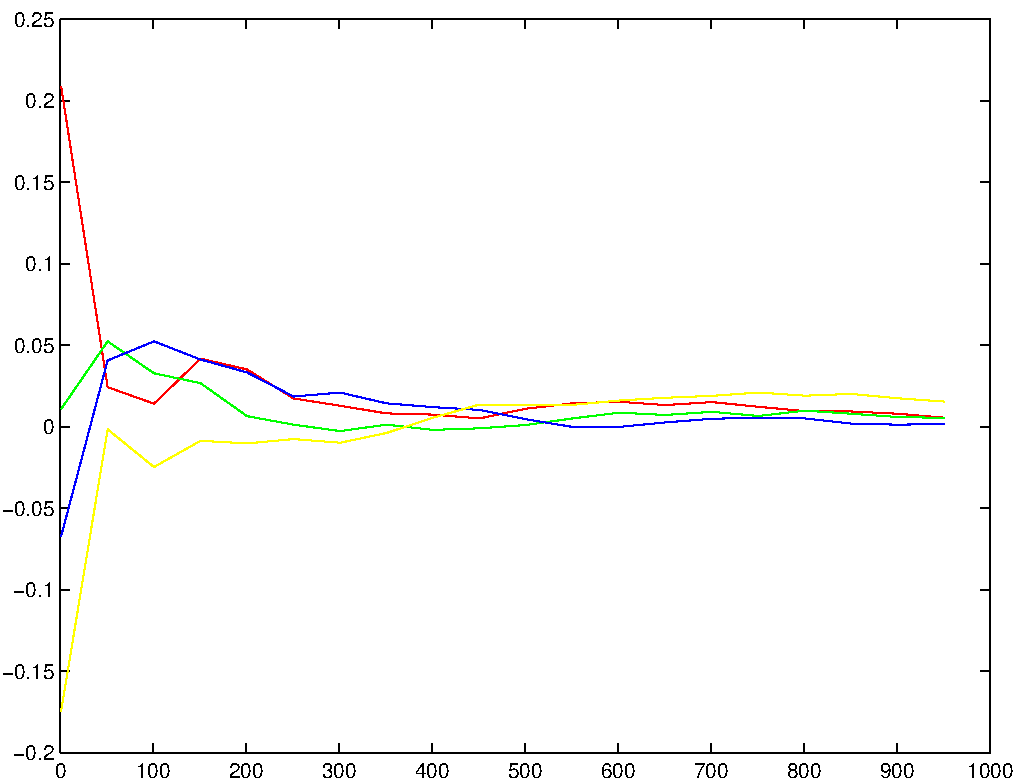
\includegraphics[width=.4\linewidth]{biasExA} &
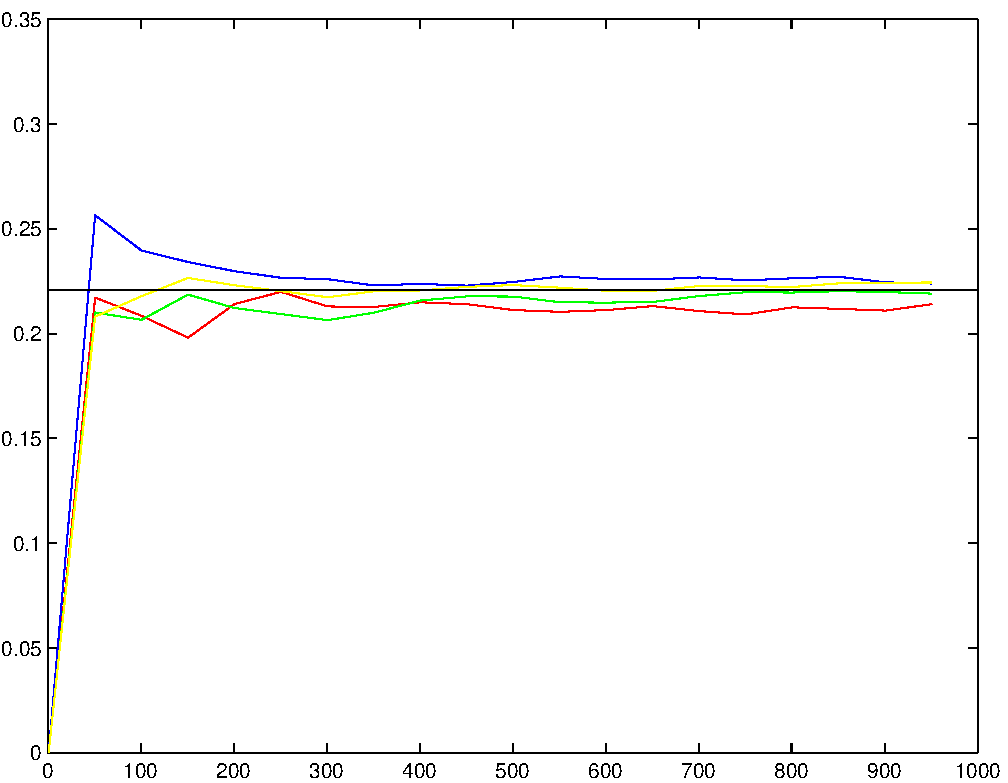
\includegraphics[width=.4\linewidth]{stdExA} \\ 
$\widehat{\mathrm{Bias}}$ & $\hat{se}_{B}$ \\
\end{tabular}
\caption{Bias and standard error bootstrap estimates w.r.t. $B$ (4 experiments have been run).}
\end{figure}

%\begin{block}{}
%you usually need to compute more $B$ bootstrap resamples to compute the bootstrap bias estimate than the bootstrap standard error. 
%\end{block}
}

%%%%%%%%%%%%%%%%%%%%%%%%%%%%%%%%%%%%%%%%%%%%%%%%%%%%%%%%%%%%%%
\frame{
\frametitle{Example of non-parametric bootstrap failure}

\begin{exampleblock}{Example B}
Considering a sample $\mathbf{x}$ drawn from a uniform  distribution $f=\mathcal{U}(0,\theta=1)$, the statistics of interest is $\hat{\theta}=\max\lbrace x_1,\cdots,x_n\rbrace$, and ${\scriptstyle\mathbf{x}=(0.5729, 0.1873, 0.5984,  0.2883,    0.8722,}$
${\scriptstyle 0.4320,    0.4896,    0.7106, 0.2754 ,   0.7637)}$.
%Assuming that $\hat{\theta}=x_1$ and that all $x_i$s are different, the probability of a replication $\hat{\theta}^{*}$ to be equal to $x_1$ is 0.632. 
\end{exampleblock}

\begin{columns}[t]
\column{.45\linewidth}
\begin{figure}[!h]
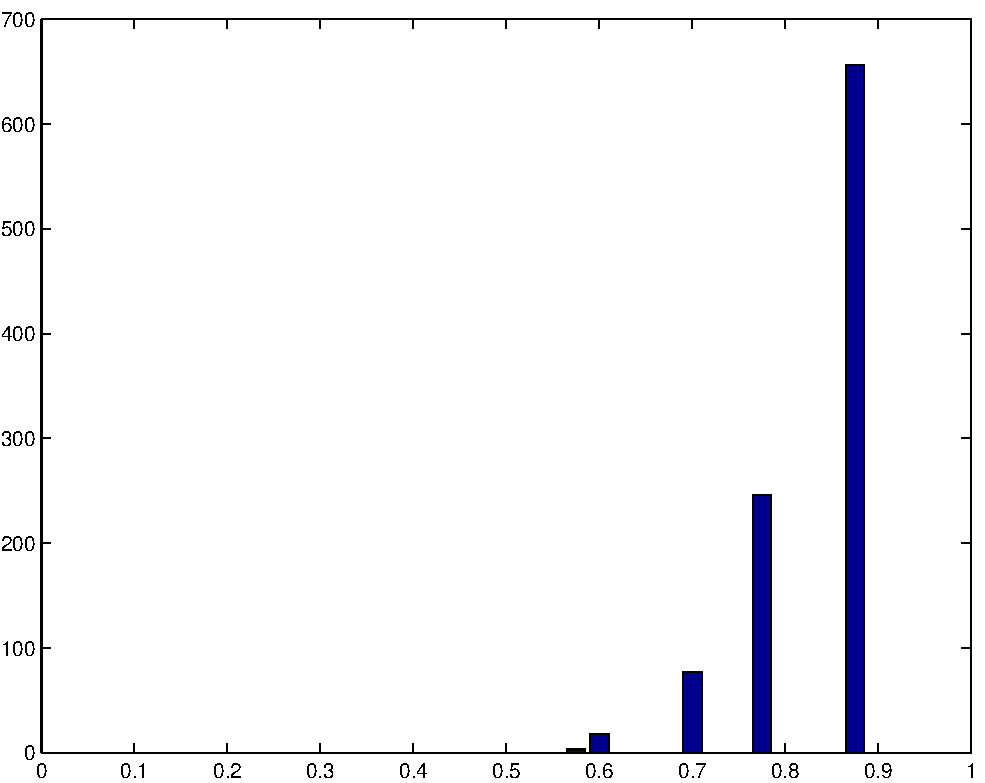
\includegraphics[width=.7\linewidth]{UniformNP.pdf} 
\caption{\tiny{Histogram of the nonparametric bootstrap replications $\hat{\theta}^{*}$ with $n=10$, $B=1000$, $\hat{\theta}=0.8722$. The maximum peak is at $\hat{\theta}=0.8722$ with a probability of $\mathcal{P}(\hat{\theta}\in \mathbf{x}^{*})= 0.6560 \approx 1-\left(1-1/n\right)^{n}= 0.6513$.}}
\end{figure} 
\column{.5\linewidth}
\begin{figure}[!h]
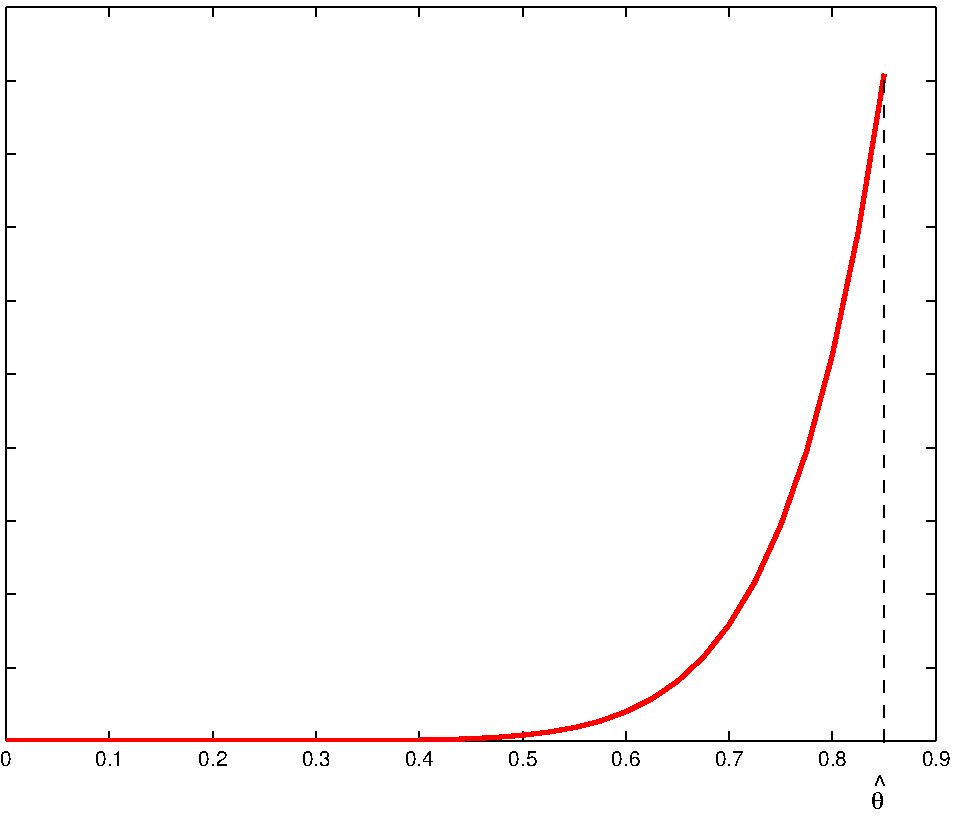
\includegraphics[width=.6\linewidth]{idealUniform.pdf} 
\caption{\tiny{Theoretical results (extreme values) says that $\mathcal{P}(\hat{\theta}^{*})=n \frac{(\hat{\theta}^{*})^{n-1}}{\hat{\theta}^{n}}$.}}
\end{figure} 
\end{columns}
}
%%%%%%%%%%%%%%%%%%%%%%%%%%%%%%%%%%%%%%%%%%%%%%%%%%%%%%%%%%%%%%
\frame{
\frametitle{Example of non-parametric bootstrap failure}
\begin{exampleblock}{Example B}
What went wrong in this example ?
\begin{itemize}
\item The empirical density function  $\hat{f}$ is not a good approximation of the true distribution $f=\mathcal{U} (0,\theta)$.

\

\item Either parametric knowledge of $f$ or some smoothing of $\hat{f}$ is needed to rectify matters.

\end{itemize}
\end{exampleblock}
}
%%%%%%%%%%%%%%%%%%%%%%%%%%%%%%%%%%%%%%%%%%%%%%%%%%%%%%%%
\frame{
\frametitle{Convergence of the bootstrap estimates}
With $\mathbf{x}=(x_1,\cdots,x_n)$, $n$ i.i.d. values, it is required:\

\

\begin{enumerate}
\item Convergence of $\hat{f}$ to $f$ for $n \rightarrow \infty$ (Glivenko-Cantelli lemma)\

\

\item Estimate $\hat{\theta}=t(\hat{f})$ is the plug-in estimate of $\theta=t(f)$\

\

\item Smoothness condition on the functional. E.g
\begin{itemize}
\item  Smooth functionals: means, variance, etc.
\item Not smooth: extreme order statistics (minimum, maximum)
\end{itemize}
\end{enumerate}
}
%%%%%%%%%%%%%%%%%%%%%%%%%%%%%%%%%%%%%%%%%%%%%%%%%%%%%%%%%%%%%%
%%%%%%%%%%%%%%%%%%%%%%%%%%%%%%%%%%%%%%%%%%%%%%%%%%%%%%%%
\frame
{
\frametitle{Parametric Bootstrap}

\begin{figure}[!h]
$$
\begin{array}{rcccr}
Real\ World & & Estimation & & Bootstrap\ World \\
&&&&\\
Prior: f\simeq \mathcal{N}(\mu,\sigma) \rightarrow \mathbf{x}  & \Rightarrow & (\overline{x},\hat{\sigma})& & \hat{f}\simeq\mathcal{N}(\overline{x},\hat{\sigma}) \rightarrow \mathbf{x}^{*} \\
&&&&\\
\downarrow &&& & \downarrow \ \\
&&&&\\
\hat{\theta} && & & \hat{\theta}^{*}\\
\end{array} 
$$
\caption{Example of parametric Bootstrap. $f$ is a normal distribution of unknown parameters $(\mu, \sigma)$. From the observed data $\mathbf{x}$ drawn from $f$, an estimation of the parameters  is performed giving $(\overline{x},\hat{\sigma})$.
$\hat{f}$ is then modelled by a normal distribution $\mathcal{N}(\overline{x},\hat{\sigma})$, from which bootstrap replications can be drawn $\mathbf{x}^{*}$.  Accuracy is inferred from observed variability of bootstrap replication $\hat{\theta}^{*}=s(\mathbf{x}^{*})$.}
\end{figure}
}

%%%%%%%%%%%%%%%%%%%%%%%%%%%%%%%%%%%%%%%%%%%%%%%%%%%%%%%%%%%%%%
\frame
{
\frametitle{Example with extreme value}
\begin{columns}[c]
\column{.45\linewidth}
\begin{exampleblock}{Example B}
We draw $B=1000$ bootstrap replication of $\hat{\theta}^{*}=\max \lbrace \mathbf{x}^{*}\rbrace$ using the parametric assumption $\mathcal{U}(0,\hat{\theta})$.

The extreme value distribution is  $\mathcal{P}(\hat{\theta}^{*})=n \frac{(\hat{\theta}^{*})^{n-1}}{\hat{\theta}^{n}}$. 
\end{exampleblock}

\column{.45\linewidth}

\begin{figure}[!h]
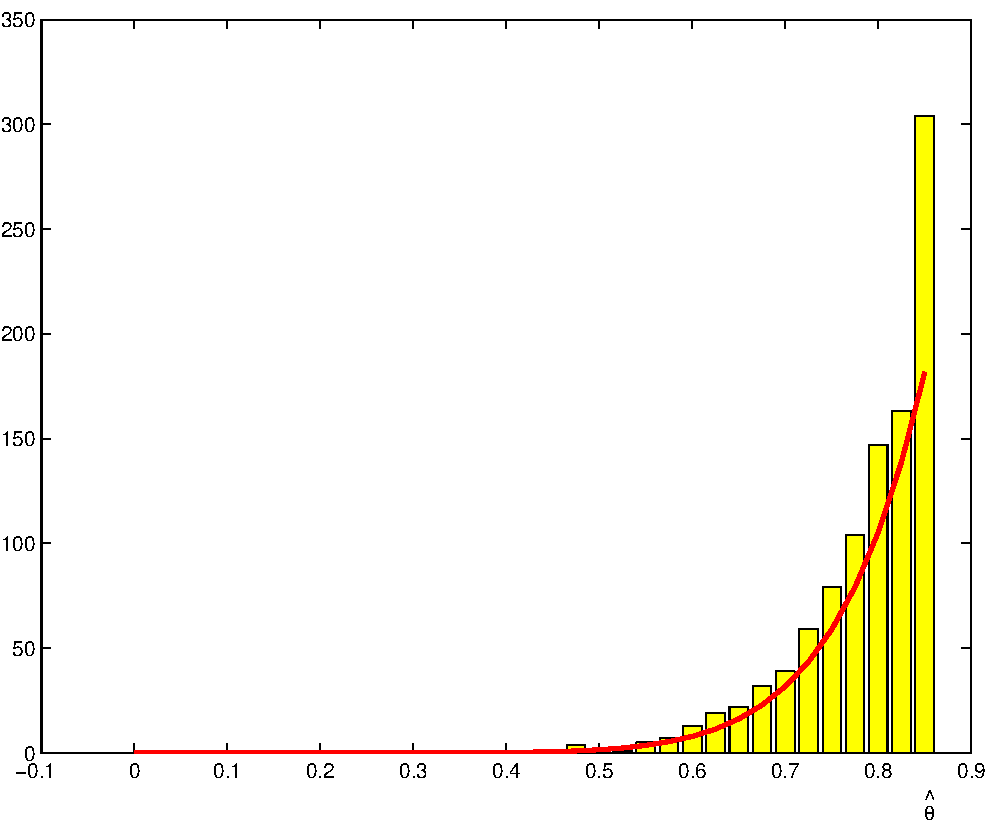
\includegraphics[width=.9\linewidth]{UniformP.pdf} 
\caption{Histogram of the parametric bootstrap replications $\hat{\theta}^{*}$ with $n=10$, $B=1000$, $\hat{\theta}=0.8722$.}
\end{figure} 

\end{columns}
}
%%%%%%%%%%%%%%%%%%%%%%%%%%%%%%%%%%%%%%%%%%%%%%%%%%%%%%%%%%%%%%
%%%%%%%%%%%%%%%%%%%%%%%%%%%%%%%%%%%%%%%%%%%%%%%%%%%%%%%%%%%%%%
\frame
{
\frametitle{The Law school example}

%\small
\begin{table}[!h]
\begin{flushleft}
\begin{tabular}{lcccccccc}
School &   1  &   2 &    3   &  4  &   5  &   6   &  7  &   8  \\
\hline
LSAT (X) & 576  &  635  &  558 &   578  &  666  &  580  &  555   & 661  \\
GPA (Y) &  3.39   &  3.30   &  2.81   &  3.03  &   3.44   &  3.07   &  3.00   &  3.43 \\

&&&&&&&&\\
\end{tabular}

\begin{tabular}{lccccccc}

School &       9   & 10   & 11 &   12  &  13  &  14   & 15 \\
\hline
LSAT (X) &  651   & 605  &  653  &  575   & 545  &  572  &  594 \\
GPA (Y) &    3.36   &  3.13  &   3.12  & 2.74   &  2.76   &  2.88   &  2.96\\

\end{tabular}
\end{flushleft}
\caption{Results of law schools admission practice  for the LSAT and GPA tests. It is believed that these scores are highly correlated. \alert{Compute the correlation and its standard error.}}
\end{table}


}



\frame
{
\frametitle{Correlation}
The correlation is defined :
$$ 
\mathrm{corr}(X,Y)=\frac{\mathbb{E}\lbrack (X -\mathbb{E}(X)) \cdot (Y -\mathbb{E}(Y))\rbrack }{\left( \mathbb{E} \lbrack (X -\mathbb{E}(X))^2 \rbrack  \cdot \mathbb{E} \lbrack (Y -\mathbb{E}(Y))^2 \rbrack \right)^{1/2}}
$$ 

Its typical estimator is:
$$
\widehat{\mathrm{corr}}(\mathbf{x},\mathbf{y})=\frac{\sum_{i=1}^{n} x_i\ y_i - n\ \overline{x}\ \overline{y}}{\lbrack \sum_{i=1}^{n}x_i^2-n\overline{x}^2 \rbrack^{1/2}\cdot \lbrack\sum_{i=1}^{n} y_i^2-n \overline{y}^2 \rbrack^{1/2} }
$$

}

%
\frame{
\frametitle{The Law school example}
\begin{itemize}
\item The estimated correlation is $\widehat{\mathrm{corr}}(\mathbf{x},\mathbf{y})=.7764$ between LSAT and GPA. 
%\item Precise theoretical formula for the standard error of the estimator is unavailable.
\end{itemize}
\begin{exampleblock}{Non-parametric Bootstrap estimate of the standard error}

\begin{table}[!h]
\begin{tabular}{l|cccccccc}
$B$ & 25 & 50 & 100 & 200 & 400 & 800 & 1600 & 3200 \\
\hline
$\hat{\mathrm{se}}_B$& .140 & .142 & .151 & .143 & .141 &.137 & .133 & .132 \\
\end{tabular}
\caption{Bootstrap estimate of standard error for $\widehat{\mathrm{corr}}(\mathbf{x},\mathbf{y})=.776$.}
\end{table}
The standard error stabilizes to $\mathrm{se}_{\hat{f}} (\widehat{\mathrm{corr}})\approx.132$.  
\end{exampleblock}
}

%%%%%%%%%%%%%%%%%%%%%%%%%%%%%%%%%%%%%%%%%%%%%%%%%%%
\frame
{
\frametitle{The Law school example}

\begin{columns}[t]
\column{0.5\linewidth}
\begin{exampleblock}{Parametric Bootstrap approach}
Assuming  that $f$ is a bivariate normale distribution, $\hat{f}_{norm}$ is estimated by computing the mean $\overline{\mathbf{z}}=(\overline{x},\overline{y})$ and the covariance matrix $\widehat{\Sigma}$ from the data.

Then $B$ samples $(\mathbf{x},\mathbf{y})^{*}$ %(of size $n=15$)
 can be drawn from $\hat{f}_{par}$ and the bootstrap estimate of the correlation coefficient can be performed. 

%$\overline{x}=600.2667$ and $\overline{y}= 3.0947$ and 
%$$ 
%\hat{\Sigma}=
%\left \lbrack
%\begin{array}{cc}
%2445  & 110.6 \\
%110.6 & 0.8302\\
%\end{array}
%\right\rbrack
%$$

\end{exampleblock}
\column{0.5\linewidth}
\begin{figure}[!h]
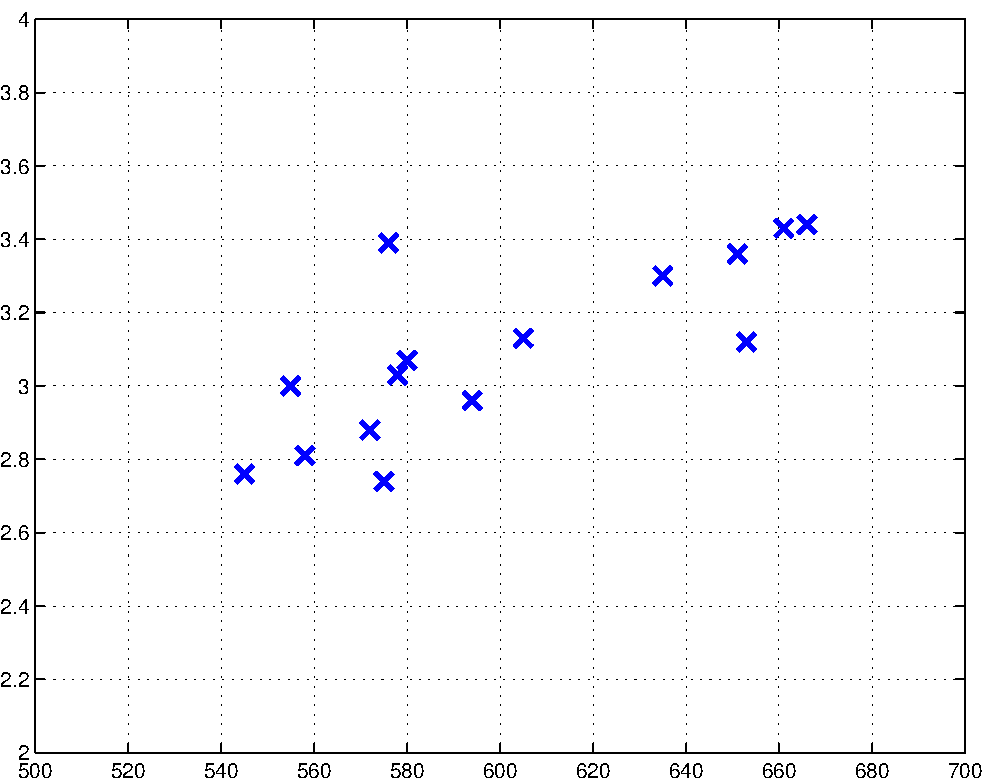
\includegraphics[width=.9\linewidth]{schoollsatgpa}
\end{figure}
\end{columns}

}


%%%%%%%%%%%%%%%%%%%%%%%%%%%%%%%%%%%%%%%%%%%%%%%%%%%%%%%%
\frame
{
\frametitle{The Law school example: Parametric Approach}

\begin{exampleblock}{Prior model}
\begin{itemize}
\item \textbf{Assumption.} $f$ is a bivariate normal density function of the form:
$$ 
f(x,y)=\frac{\exp\left\lbrack -\frac{(\mathbf{z}-\pmb{\mu}_{zf})^{T} \Sigma^{-1} (\mathbf{z}-\pmb{\mu}_{zf})}{2} 
\right\rbrack
}{(2\pi) |\det(\Sigma)|^{1/2}}
$$ 
with 
$
\mathbf{z}=
\left(
\begin{array}{c}
x\\
y\\
\end{array}\right)
$
\item \textbf{Problem.} The parameters, mean  $\pmb{\mu}_{zf}=(\mu_{xf},\mu_{yf})$ and  the covariance matrix $\Sigma$, are unknown. 
\end{itemize}
\end{exampleblock}
}

%%%%%%%%%%%%%%%%%%%%%%%%%%%%%%%%%%%%%%%%%%%%%%%%%%%%%%%%%
\frame
{
\frametitle{The Law school example: Parametric Approach}

\begin{exampleblock}{Estimate of the parametric p.d.f.}


The parametric  p.d.f. is estimated by:
$$ 
\hat{f}_{par}(x,y)=\frac{\exp\left\lbrack -\frac{(\mathbf{z}-\overline{\mathbf{z}})^{T} \overline{\Sigma}^{-1} (\mathbf{z}-\overline{\mathbf{z}})}{2} 
\right\rbrack
}{(2\pi) |\det(\overline{\Sigma})|^{1/2}}
$$
Means are $\overline{\mathbf{z}}=(\overline{x}=\frac{\sum_{i=1}^n x_i}{n},\overline{y}=\frac{\sum_{i=1}^n y_i}{n})$. 
The covariance matrix is defined as:
$$
\overline{\Sigma}=\frac{1}{n-1} \left\lbrack
\begin{array}{cc}
\sum_{i=1}^{n} (x_i-\overline{x})^2 & \sum_{i=1}^{n} (x_i-\overline{x})  (y_i-\overline{y})\\
&\\
\sum_{i=1}^{n} (x_i-\overline{x})  (y_i-\overline{y}) & \sum_{i=1}^{n} (y_i-\overline{y})^2 \\
\end{array}
\right\rbrack
$$
The mean is $\overline{\mathbf{z}}=(\overline{x}=600.3,\overline{y}=3.1)$ and
$
\overline{\Sigma}=
\left\lbrack
\begin{array}{cc}
1747 & 0.0079\\
0.0079 & 0.0001\\
\end{array}
\right\rbrack
$
\end{exampleblock}
}
%%%%%%%%%%%%%%%%%%%%%%%%%%%%%%%%%%%%%%%%%%%%%%%%%%%%%%%%
\frame{
\frametitle{Parametric Bootstrap estimate of standard error}

\begin{beamercolorbox}[wd=\linewidth, rounded=true,shadow=true]{postit}
\begin{enumerate}
\item Using the prior assumption and the available observation $\mathbf{x}=(x_1,x_2,\cdots,x_n)$, estimate $\hat{f}_{par}$
\item Instead of sampling with replacement from the data $\mathbf{x}$, draw $B$ samples $\mathbf{x}^{*(b)}$ of size $n$ from $\hat{f}_{par}$
\item Evaluate the bootstrap replications:
$$ 
\hat{\theta}^{*}(b)=s(\mathbf{x}^{*(b)}), \quad \forall b \in \lbrace 1,\cdots,B \rbrace
$$

\item Estimate the standard error $\mathrm{se}_{f}(\hat{\theta})$ by the standard deviation of the $B$ replications:
$$ 
\hat{\mathrm{se}}_{B}=\left\lbrack \frac{\sum_{b=1}^{B}\lbrack \hat{\theta}^{*}(b)-\hat{\theta}^{*}(\cdot)\rbrack^{2}}{B-1} \right\rbrack^{\frac{1}{2}}
$$
where $\hat{\theta}^{*}(\cdot)=\frac{\sum_{b=1}^{B} \hat{\theta}^{*}(b)}{B}$.
\end{enumerate}
\end{beamercolorbox}
}

%%%%%%%%%%%%%%%%%%%%%%%%%%%%%%%%%%%%%%%%%%%%%%%%%%%%%%%%
\frame{
\frametitle{Parametric Bootstrap estimate of the bias}

\begin{beamercolorbox}[wd=\linewidth, rounded=true,shadow=true]{postit}
\begin{enumerate}
\item Using the prior assumption and the available observation $\mathbf{x}=(x_1,x_2,\cdots,x_n)$, estimate $\hat{f}_{par}$
\item Instead of sampling with replacement from the data $\mathbf{x}$, draw $B$ samples $\mathbf{x}^{*(b)}$ of size $n$ from $\hat{f}_{par}$
\item Evaluate the bootstrap replications:
$$ 
\hat{\theta}^{*}(b)=s(\mathbf{x}^{*(b)}), \quad \forall b \in \lbrace 1,\cdots,B \rbrace
$$

\item Estimate the bias: 
$$ 
\widehat{\mathrm{Bias}}_{B}=\hat{\theta}^{*}(\cdot)-\hat{\theta}
$$
where $\hat{\theta}^{*}(\cdot)=\frac{\sum_{b=1}^{B} \hat{\theta}^{*}(b)}{B}$.
\end{enumerate}
\end{beamercolorbox}
}
%%%%%%%%%%%%%%%%%%%%%%%%%%%%%%%%%%%%%%%%%%%%%%%%%%%%%%%%
\frame{
\frametitle{Resampling and Monte Carlo Simulation}

\begin{itemize}
\item  In resampling, one could do all possible combinations, but it would be too time-consuming and computing-intensive. \

\

\item The alternative is Monte Carlo sampling, which restricts the resampling to a certain number. It is used in the computation of the bootstrap samples in the nonparametric case when a random index $(i_1,\cdots,i_n)$ is simulated from the uniform distribution $[1;n]$ ($\mathbf{x}^{*}=(x_{i_1},\cdots,x_{i_1})$). 

\

\item The data could be totally hypothetical in Monte Carlo simulation, while in the resampling,  the simulation is based upon some real observation $\mathbf{x}=(x_1,\cdots,x_n)$.

\

\item In the parametric case, the bootstrap samples from $\hat{f}_{par}$ are computed using Monte Carlo methods and are not anymore resamples from $\mathbf{x}$.  

\end{itemize}
}
%%%%%%%%%%%%%%%%%%%%%%%%%%%%%%%%%%%%%%%%%%%%%%%%%%%%%%%%
\frame{
\frametitle{The Law school example: Parametric Bootstrap}
\begin{columns}[c]
\column{0.5\linewidth}
For $B=3200$ bootstrap replications, we compute
$\widehat{\mathrm{corr}}^{*}(\cdot)=0.7661$ and the parametric bootstrap standard error $0.1169$. 

\column{0.5\linewidth}
\begin{figure}[!h]
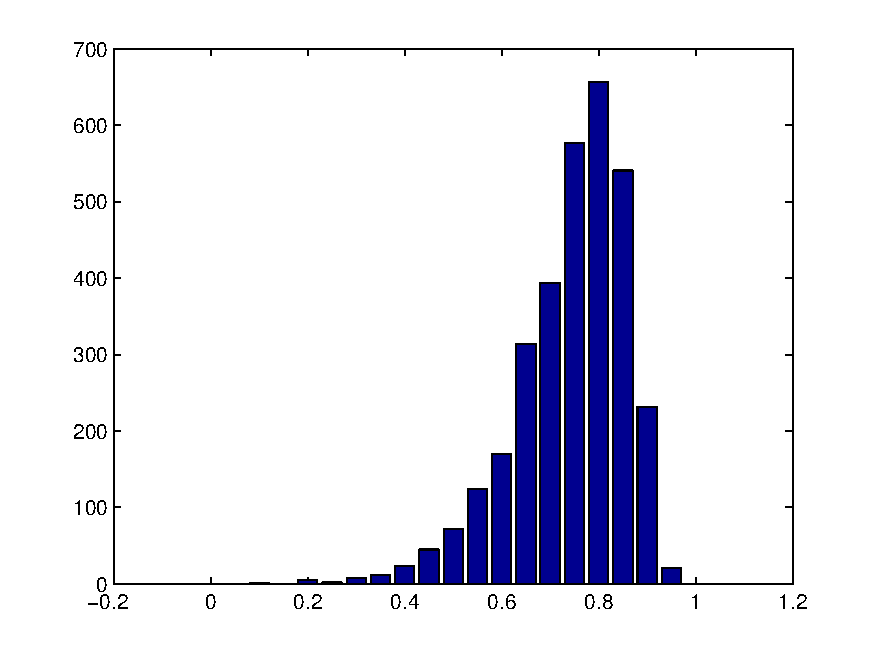
\includegraphics[width=\linewidth]{correlationparametricbootstrap3200}
\caption{Histogram of 3200 parametric bootstrap replication of corr $\widehat{\mathrm{corr}}(x^{*},y^{*})$.}
\end{figure}

\end{columns}
}

%%%%%%%%%%%%%%%%%%%%%%%%%%%%%%%%%%%%%%%%%%%%%%%%%%%%%%%
\frame{
\frametitle{The Law school example: Conclusion}

\begin{itemize}
\item The textbook formula for  the correlation coefficient is:
$$
\mathrm{se}_{\hat{f}}=(1-\widehat{\mathrm{corr}}^2)/\sqrt{n-3}
$$
With $\widehat{\mathrm{corr}}(\mathbf{x},\mathbf{y})=0.7764$, the standard error is $se_f=0.1147$.
\item The non-parametric bootstrap  standard error for $B=3200$ is $0.132$.
\item The parametric bootstrap  standard error for $B=3200$ is $0.1169$.

\end{itemize}

}


%%%%%%%%%%%%%%%%%%%%%%%%%%%%%%%%%%%%%%%%%%%%%%%%%%%%%%%%
\frame{
\frametitle{Parametric and nonparametric bootstrap estimates}

\begin{itemize}
\item The nonparametric approach leads to a finite number of possible replications $\hat{\theta}^{*}(b)$. In fact considering $n$ distinct values in $\mathbf{x}=(x_1,\cdots,x_n)$, the maximum number of \textit{different} bootstrap samples (and replications) is \footnote{$n=11$, $B_{max}=652716$: big enough to minimize the effect of the discreteness in the nonparametric approach.}:
$$
B_{max}=\left(
\begin{array}{c}
2n-1\\
n-1\\
\end{array}\right)=\frac{(2n-1)!}{n! (n-1)!}
$$     
\item The parametric approach has an unlimited number of different bootstrap samples and replications.
\end{itemize}

}
%%%%%%%%%%%%%%%%%%%%%%%%%%%%%%%%%%%%%%%%%%%%%%%%%%%%%%%%%%%%%%%%%%%%%%%%%%
\frame{
\frametitle{When might the (parametric and non parametric) bootstrap fail?}
Bootstrap might fail when:
\begin{itemize}
\item incomplete data (missing data) : incomplete observation $\mathbf{x}$
\item dependent data (e.g. correlated time series) $\mathbf{x}=(x_1,\cdots,x_n)$ dependent
\item dirty data (outliers) : noisy observation $\mathbf{x}$
\end{itemize}

\begin{block}{}
For a critical view on bootstrap, see the publication \textit{Exploring the limits
of bootstrap} edited by Le Page and Billard 1990 (ISBN: 0-471-53631-8).
\end{block}
}

%%%%%%%%%%%%%%%%%%%%%%%%%%%%%%%%%%%%%%%%%%%%%%%%%%%%%%%%
\frame{
\frametitle{Conclusion}
\begin{itemize}
\item In  parametric bootstrap, $\hat{f}_{par}$ is not anymore the empirical density function.  

\

\item If the prior information on $f$ is accurate, then  $\hat{f}_{par}$ estimates better $f$ than the empirical p.d.f.. In this case the parametric bootstrap gives better estimation for the standard errors.

\

\item Most of the time, the point  of making assumptions is to derive the textbook formulas.  \\

\textit{All models are wrong, but some are useful}- G.E.P. Box, 1979.

\

\item On the other hand, non-parametric bootstrap allows the computation of accurate standard errors (in many cases) without making any prior assumption.
\end{itemize}
}
%%%%%%%%%%%%%%%%%%%%%%%%%%%%%%%%%%%%%%%%%%%%%%%%%%%%%%%%
\frame{
\frametitle{Conclusion}
\begin{itemize}
\item In non-parametric mode, the bootstrap method relieves the analyst from choosing a parametric assumption about the form of the underlying density function $f$.

\

\item In both case, bootstrap can provide answers for problem for which no textbook formulae exists.
\end{itemize}
}


%%%%%%%%%%%%%%%%%%%%%%%%%%%
\section{Jackknife}
\frame{
\frametitle{Introduction to resampling methods}
\begin{itemize}
\item Definitions and Problems
\item Non-Parametric Bootstrap
\item Parametric Bootstrap
\item \textbf{Jackknife}
\item Permutation tests
\item Cross-validation
\end{itemize}
}
\frame
{
\frametitle{Introduction}

The bootstrap method is not always the best one. One main reason is that the bootstrap samples are generated from $\hat{f}$ and not from $f$. \alert{Can we find samples/resamples exactly generated from $f$?}

\begin{itemize}
\item If we look for samples of size $n$, then the answer is \alert{no}!
\item If we look for samples of size $m$ ($m<n$), then we can indeed find (re)samples of size $m$ exactly generated from $f$ simply by looking at different subsets of our original sample $\mathbf{x}$! 
\end{itemize}

Looking at different subsets of our original sample amounts to sampling without replacement from observations $x_1,\cdots,x_n$ to get (re)samples (now called \alert{subsamples}) of size $m$. This leads us to subsampling and the jackknife.  
}

\frame
{
\frametitle{Jackknife}

\begin{itemize}
\item  The jackknife has been proposed by Quenouille in mid 1950's.

\

\item In fact, the jackknife predates the bootstrap. 

\

\item The jackknife (with $m=n-1$) is less computer-intensive than the bootstrap. 

\

\item \textit{Jackknife} describes a swiss penknife, easy to carry around. By analogy, Tukey (1958) coined the term in statistics as a general approach for testing hypotheses and calculating confidence intervals.  


\end{itemize}

}
%%%%%%%%%%%%%%%%%%%%%%%%%%%%%%%%%%%%%%%%%%%%%%%%%%%
\frame
{
\frametitle{Jackknife samples}

\begin{definition}
The \alert{Jackknife samples} are computed by leaving out one observation $x_i$ from $\mathbf{x}=(x_{1},x_{2},\cdots,x_{n})$ at a time:
$$
\mathbf{x}_{(i)}=(x_{1},x_{2},\cdots,x_{i-1},x_{i+1},\cdots,x_{n})
$$ 
\end{definition}

\begin{beamercolorbox}[wd=\linewidth, rounded=true,shadow=true]{postit}
\begin{itemize}
\item The dimension of the jackknife sample $\mathbf{x}_{(i)}$ is $m=n-1$  
\item $n$  different Jackknife samples :  $\lbrace\mathbf{x}_{(i)}\rbrace_{i=1\cdots n}$.
\item No sampling method needed to compute the $n$  jackknife samples.

\end{itemize}
\end{beamercolorbox}
\begin{block}{}
\tiny{Available BOOTSTRAP MATLAB TOOLBOX, by Abdelhak M. Zoubir and D. Robert Iskander, 
\href{http://www.csp.curtin.edu.au/downloads/bootstrap_toolbox.html}{http://www.csp.curtin.edu.au/downloads/bootstrap\_toolbox.html}}
\end{block}
}

%%%%%%%%%%%%%%%%%%%%%%%%%%%%%%%%%%%%%%%%%%%%%%%%%%%%%%
\frame
{
\frametitle{Jackknife replications}

\begin{definition}
The ith \alert{jackknife replication} $\hat{\theta}_{(i)}$ of the statistic $\hat{\theta}=s(\mathbf{x})$ is:
$$ 
\hat{\theta}_{(i)}=s(\mathbf{x}_{(i)}),\quad \forall i=1,\cdots,n
$$
\end{definition}

\begin{exampleblock}{Jackknife replication of the mean}


$$
\begin{array}{ll}
s(\mathbf{x}_{(i)})&=\frac{1}{n-1}\sum_{j\neq i } x_j\\
&\\
&=\frac{(n\overline{x}-x_i)}{n-1} \\
&\\
&=\overline{x}_{(i)}\\
\end{array}
$$

\end{exampleblock}
}
%%%%%%%%%%%%%%%%%%%%%%%%%%%%%%%%%%%%%%%%%%%%%%%%%%%%
\frame
{
\frametitle{Jackknife estimation of the standard error}


\begin{beamercolorbox}[wd=\linewidth, rounded=true,shadow=true]{postit}

\begin{enumerate}
\item Compute the $n$ jackknife subsamples $\mathbf{x}_{(1)}, \cdots,\mathbf{x}_{(n)}$ from $\mathbf{x}$.

\

\item Evaluate the $n$ jackknife replications $\hat{\theta}_{(i)}=s(\mathbf{x}_{(i)})$.

\

\item The \alert{jackknife estimate of the standard error} is defined by:
$$
\hat{\mathrm{se}}_{jack}=\left \lbrack \frac{n-1}{n} \sum_{i=1}^{n} (\hat{\theta}_{(\cdot)}-\hat{\theta}_{(i)})^{2}\right\rbrack^{1/2}
$$
where $\hat{\theta}_{(\cdot)}=\frac{1}{n}\sum_{i=1}^{n} \hat{\theta}_{(i)}$.

\end{enumerate}
\end{beamercolorbox}
}
%%%%%%%%%%%%%%%%%%%%%%%%%%%%%%%%%%%%%%%%%%%%%%%%%%%%
\frame
{
\frametitle{Jackknife estimation of the standard error of the mean}

For $\hat{\theta}=\overline{x}$, it is easy to show that: 
$$
\left\lbrace
\begin{array}{l}
\overline{x}_{(i)}=\frac{n\overline{x}-x_i}{n-1}\\
\\
\overline{x}(\cdot)=\frac{1}{n}\sum_{i=1}^{n} \overline{x}_{(i)}=\overline{x}\\
\end{array}
\right.
$$
 Therefore:
$$
\begin{array}{ll}
\widehat{\mathrm{se}}_{jack}&=\left\lbrace \sum_{i=1}^n \frac{(x_i-\overline{x})^2}{(n-1)n} \right\rbrace^{1/2}\\
&\\
& =  \frac{\overline{\sigma}}{\sqrt{n}}\\
\end{array}
$$
where $\overline{\sigma}$ is the unbiased variance. 

}
%%%%%%%%%%%%%%%%%%%%%%%%%%%%%%%%%%%%%%%%%%%%%%%%%%%%
\frame
{
\frametitle{Jackknife estimation of the standard error}

\begin{itemize}
\item The factor $\frac{n-1}{n}$ is much larger than $\frac{1}{B-1}$ used in bootstrap. 

\

\item Intuitively this inflation factor is needed because jackknife deviation $(\hat{\theta}_{(i)}-\hat{\theta}_{(\cdot)})^{2}$ tend to be smaller than the bootstrap  $(\hat{\theta}^{*}(b)-\hat{\theta}^{*}(\cdot))^{2}$ (the jackknife sample is more similar to the original data $\mathbf{x}$ than the bootstrap).  

\

\item In fact, the factor $\frac{n-1}{n}$ is derived by considering the special case $\hat{\theta}=\overline{x}$ (somewhat arbitrary convention).  
\end{itemize}
}
%%%%%%%%%%%%%%%%%%%%%%%%%%%%%%%%%%%%%%%%%%%%%%%%%%%%
\frame
{
\frametitle{Comparison of Jackknife and Bootstrap on an example}
\begin{exampleblock}{Example A: $\hat{\theta}=\overline{x}$}
%We consider $\hat{\theta}=\overline{x}$ computed over an observation $\mathbf{x}$ of $n=100$ values sampled from the distribution: 
 $f(x)=0.2\ \mathcal{N}(\scriptstyle \mu=1,\sigma=2 \displaystyle) +0.8\  \mathcal{N}( \scriptstyle\mu=6,\sigma=1 \displaystyle)
$   $\rightsquigarrow\mathbf{x}=(x_1,\cdots,x_{100})$. 
\begin{itemize}
\item  Bootstrap standard error and bias w.r.t. the number $B$ of bootstrap samples: 
\end{itemize}
%\begin{table}[!h]
\begin{tabular}{|c|c|c|c|c|c|c|c|}
\hline
$B$& 10& 20 & 50 & 100 & 500 & 1000  & 10000\\
\hline
$\widehat{\mathrm{se}}_{B}$& \small{0.1386} & \small{0.2188} & \small{0.2245} & \small{0.2142} & \small{0.2248}& \small{0.2212} & \small{0.2187}\\
\hline
$\widehat{\mathrm{Bias}}_{B}$ & \small{0.0617} & \small{-0.0419} & \small{0.0274} & \small{-0.0087} & \small{-0.0025} &  \small{0.0064} & \small{0.0025} \\
%\small{-0.1062} & \small{-0.0532} & \small{-0.0364} &  \small{-0.0199} & \small{-0.0003} & \small{-0.001} & \small{-0.002}\\
\hline
\end{tabular}

\

%\caption{\small{Bootstrap standard error and bias w.r.t. the number $B$ of bootstrap samples.}}
%\end{table}
\begin{itemize}
\item Jackknife: $\widehat{\mathrm{se}}_{jack}=0.2207$ and  $\widehat{\mathrm{Bias}}_{jack}= 0$

\

\item Using textbook formulas:  $ \mathrm{se}_{\hat{f}}=\frac{\hat{\sigma}}{\sqrt{n}}=0.2196$  ($\frac{\overline{\sigma}}{\sqrt{n}}=0.2207$).
\end{itemize}
\end{exampleblock}

}

%%%%%%%%%%%%%%%%%%%%%%%%%%%%%%%%%%%%%%%%%%%%%%%%%%%%
\frame
{
\frametitle{Jackknife estimation of the bias}


\begin{beamercolorbox}[wd=\linewidth, rounded=true,shadow=true]{postit}
\begin{enumerate}
\item Compute the $n$ jackknife subsamples $\mathbf{x}_{(1)}, \cdots,\mathbf{x}_{(n)}$ from $\mathbf{x}$.

\

\item Evaluate the $n$ jackknife replications $\hat{\theta}_{(i)}=s(\mathbf{x}_{(i)})$.

\

\item The \alert{jackknife estimation of the bias} is defined as:
$$
\widehat{\mathrm{Bias}}_{jack}=(n-1)(\hat{\theta}_{(\cdot)}-\hat{\theta})
$$
where $\hat{\theta}_{(\cdot)}=\frac{1}{n}\sum_{i=1}^{n} \hat{\theta}_{(i)}$. 

\end{enumerate}
%This formula applies only to plug-in statistics $\hat{\theta}=t(\hat{F})$.

\end{beamercolorbox}
}
%%%%%%%%%%%%%%%%%%%%%%%%%%%%%%%%%%%%%%%%%%%%%%%%%%%%
\frame
{
\frametitle{Jackknife estimation of the bias}

\begin{itemize}
\item Note the inflation factor $(n-1)$ (compared to the bootstrap bias estimate).

\

\item $\hat{\theta}=\overline{x}$ is unbiased so the correspondence is done considering the plug-in estimate of the variance $\hat{\sigma}^2=\frac{\sum_{i=1}^n (x_i-\overline{x})^2}{n}$. 

\

\item The jackknife estimate of the bias for the plug-in estimate of the variance is then:
$$    
\widehat{\mathrm{Bias}}_{jack}=\frac{\overline{-\sigma}^2}{n}
$$
\end{itemize}
}
%%%%%%%%%%%%%%%%%%%%%%%%%%%%%%%%%%%%%%%%%%%%%%%%%%%%
\frame
{
\frametitle{Histogram of the replications} 

\begin{exampleblock}{Example A}
\begin{figure}[!h]
\begin{tabular}{p{5cm}p{5cm}}
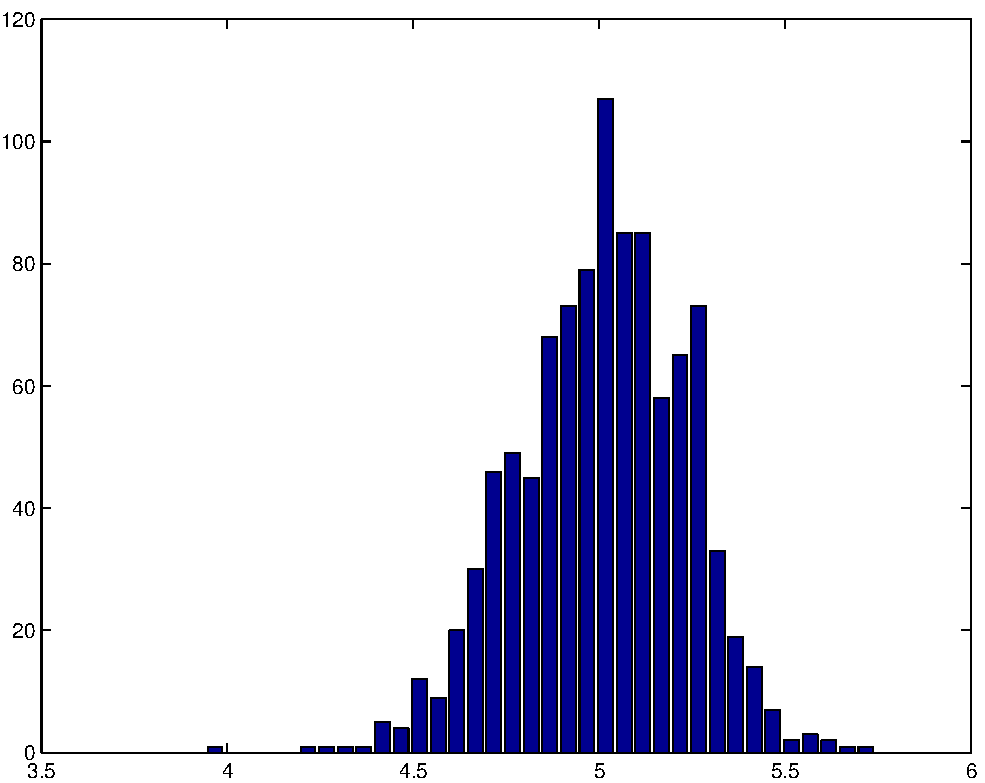
\includegraphics[width=5cm]{histobootreplications}&
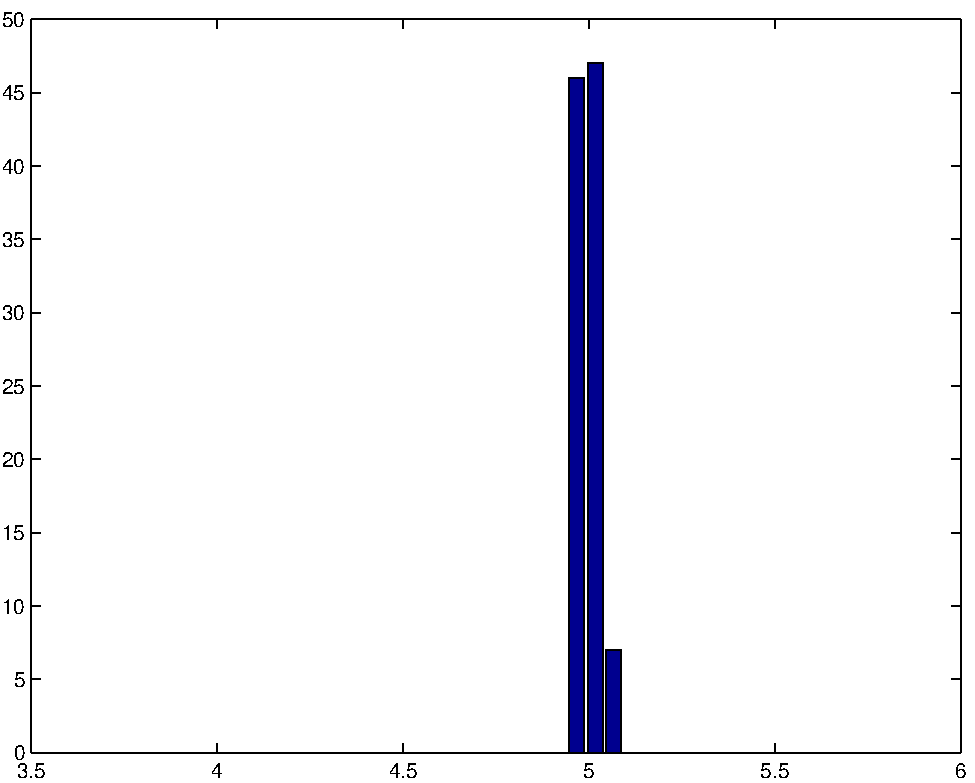
\includegraphics[width=5cm]{histojackreplications}\\
\end{tabular}
\caption{Histograms of the bootstrap replications $\lbrace \hat{\theta}^{*}(b)\rbrace_{b\in \lbrace 1,\cdots,B=1000 \rbrace}$ (left), and the jackknife replications $\lbrace \hat{\theta}_(i)\rbrace_{i\in \lbrace 1,\cdots,n=100 \rbrace}$ (right).}
\end{figure}
\end{exampleblock}
}
%%%%%%%%%%%%%%%%%%%%%%%%%%%%%%%%%%%%%%%%%%%%%%%%%%%%
\frame
{
\frametitle{Histogram of the replications} 
\begin{exampleblock}{Example A}
\begin{figure}[!h]
\begin{tabular}{p{5cm}p{5cm}}
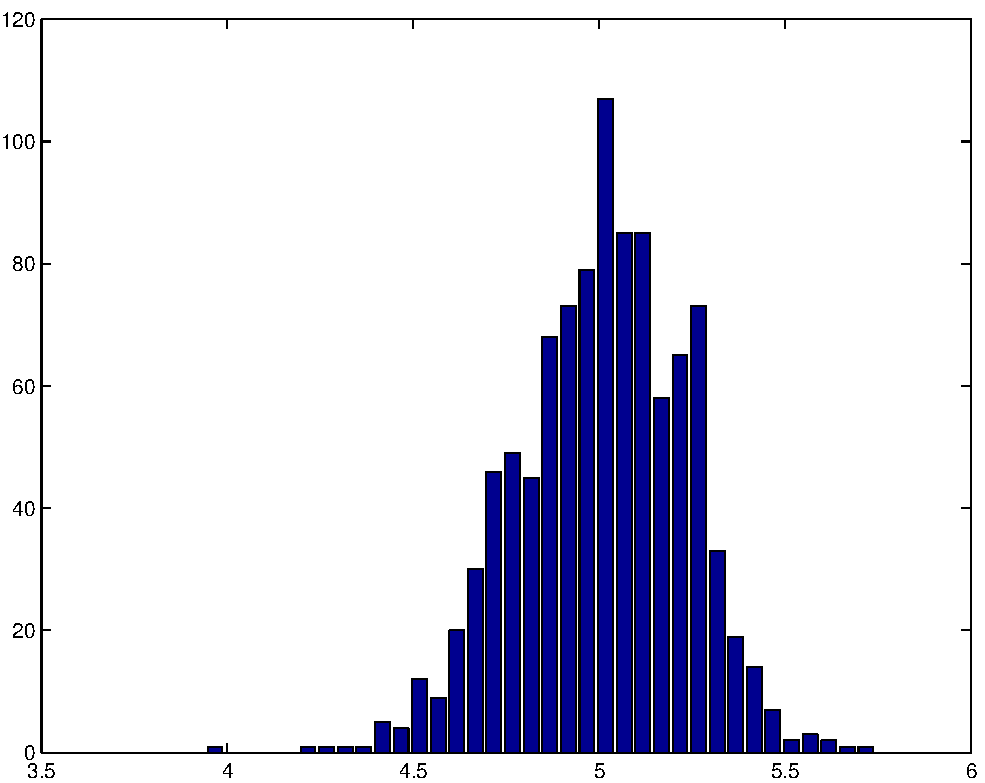
\includegraphics[width=5cm]{histobootreplications}&
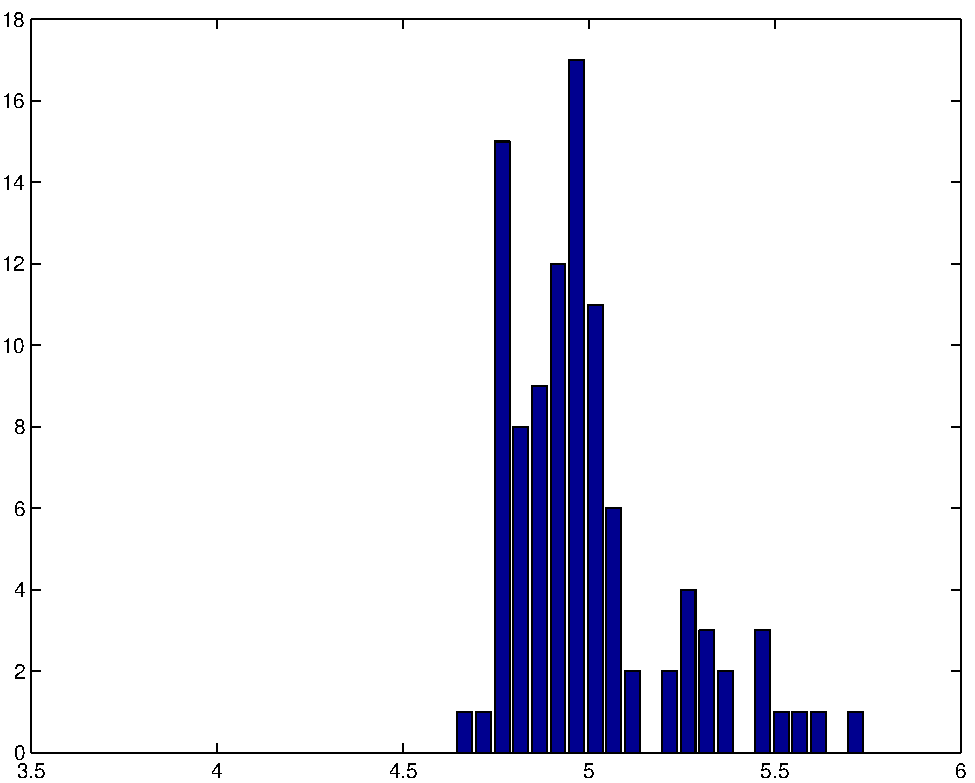
\includegraphics[width=5cm]{histojackreplicationsinflated}\\
\end{tabular}
\caption{Histograms of the bootstrap replications $\lbrace \hat{\theta}^{*}(b)\rbrace_{b\in \lbrace 1,\cdots,B=1000 \rbrace}$ (left), and the inflated jackknife replications $\lbrace \sqrt{n-1} (\hat{\theta}_{(i)}-\hat{\theta}_{(\cdot)})+ \hat{\theta}_{(\cdot)} \rbrace_{i\in \lbrace 1,\cdots,n=100 \rbrace}$ (right).}
\end{figure}
\end{exampleblock}

}
%%%%%%%%%%%%%%%%%%%%%%%%%%%%%%%%%%%%%%%%%%%%%%%%%%
\frame{
\frametitle{Relationship between jackknife and bootstrap}

\begin{itemize}
\item When $n$ is small, it is easier (faster) to compute the $n$ jackknife replications.

\

\item However the jackknife uses less information (less samples) than the bootstrap.

\

\item In fact, the jackknife is an  approximation to the bootstrap!   
\end{itemize}
}
%%%%%%%%%%%%%%%%%%%%%%%%%%%%%%%%%%%%%%%%%%%%%%%%%%%%
\frame
{
\frametitle{Relationship between jackknife and bootstrap}

\begin{itemize}
\item Considering a linear statistic : 
$$
\begin{array}{ll}
\hat{\theta}&=s(\mathbf{x})=\mu+\frac{1}{n} \sum_{i=1}^{n}\alpha(x_i)\\
&\\
&=\mu+\frac{1}{n} \sum_{i=1}^{n}\alpha_i\\
\end{array}
$$
\begin{exampleblock}{Mean $\hat{\theta}=\overline{x}$}
The mean is linear $\mu=0$ and $\alpha(x_i)=\alpha_i=x_i,\quad \forall i\in \lbrace 1,\cdot,n\rbrace$.
\end{exampleblock}
\item There is no loss of information in using the jackknife to compute the standard error (compared to the bootstrap) for a linear statistic. Indeed the knowledge of the $n$ jackknife replications $\lbrace \hat{\theta}_{(i)} \rbrace$, gives the value of $\hat{\theta}$ for any bootstrap data set. 
 
\item For non-linear statistics, the jackknife makes a linear approximation to the bootstrap  for the standard error. 

\end{itemize}

}
%%%%%%%%%%%%%%%%%%%%%%%%%%%%%%%%%%%%%%%%%%%%%%%%%%%%
\frame
{
\frametitle{Relationship between jackknife and bootstrap}


\begin{itemize}
\item Considering a quadratic  statistic
$$
\begin{array}{ll}
\hat{\theta}&=s(\mathbf{x})=\mu+\frac{1}{n} \sum_{i=1}^{n}\alpha(x_i)+\frac{1}{n^2} \beta(x_i,x_j)\\
\end{array}
$$
\begin{exampleblock}{Variance $\hat{\theta}=\hat{\sigma}^{2}$}
$\hat{\sigma}^{2}=\frac{1}{n}\sum_{i=1}^{n}(x_i-\overline{x})^2$ is a quadratic statistic.
\end{exampleblock}

\item Again the knowledge of the $n$ jackknife replications $\lbrace s(\hat{\theta}_{(i)}) \rbrace$, gives the value of $\hat{\theta}$ for any bootstrap data set. The jackknife and bootstrap estimates of the bias agree for quadratic statistics. 
\end{itemize}

}
%%%%%%%%%%%%%%%%%%%%%%%%%%%%%%%%%%%%%%%%%%%%%%%%%%%%
\frame
{
\frametitle{Relationship between jackknife and bootstrap}
\begin{exampleblock}{The Law school example: $\hat{\theta}=\widehat{\mathrm{corr}}(\mathbf{x},\mathbf{y})$.}
The correlation is a non linear statistic.
\begin{itemize}
\item From B=3200 bootstrap replications, $\hat{\mathrm{se}}_{B=3200}=0.132$. 
% $\mathbb{E}\lbrack\hat{\mathrm{se}}_{B=100}\rbrack=0.132$. 
%(and standard deviation $0.0117$).

\

\item From $n=15$ jackknife replications, $\hat{\mathrm{se}}_{jack}= 0.1425$.

\

\item Textbook formula: 
$\mathrm{se}_{\hat{f}}=(1-\widehat{\mathrm{corr}}^2)/\sqrt{n-3}=0.1147$
\end{itemize}
\end{exampleblock}

}
%%%%%%%%%%%%%%%%%%%%%%%%%%%%%%%%%%%%%%%%%%%%%%%%%%%%
\frame{
\frametitle{Failure of the jackknife}

The jackknife can fail if the estimate $\hat{\theta}$ is not smooth (i.e. a small change in the data can cause a large change in the statistic).
A simple non-smooth statistic is the median.
\begin{exampleblock}{On the mouse data}
Compute the jackknife replications of the median $\mathbf{x}_{Cont}=(10,27,31,40,46,50,52,104,146)$ (Control group data).
\begin{itemize}
\item  You should find 48,48,48,48,45,43,43,43,43 \footnote{The median of an even number of data points is the average of the middle 2 values.}. 

\

\item Three different values appears as  a consequence of a lack of smoothness of the median\footnote{the median is not a differentiable function of $x$.}. 
\end{itemize} 
\end{exampleblock}
}
%%%%%%%%%%%%%%%%%%%%%%%%%%%%%%%%%%%%%%%%%%%%%%%%%%%%
%\frame
%{
%\frametitle{Relationship between jackknife and bootstrap}
%
%\begin{table}[!h]
%\begin{tabular}{p{2cm}|p{2cm}|p{2cm}|p{2cm}|p{2cm}}
%$\hat{\theta}$ & linear & quadratic & non-linear (but smooth) & non-smooth\\
%\hline
%jackknife se &  agree with bootstrap  & linear approx. of bootstrap se &  
%linear approx. of bootstrap se & fails \\
% \hline
%jackknife bias & agree with bootstrap bias & agree with bootstrap bias & approx. of bootstrap & fails\\
%  \end{tabular}
%\end{table}
%}

%%%%%%%%%%%%%%%%%%%%%%%%%%%%%%%%%%%%%%%%%%%%%%%%%%%%
%\frame{
%\frametitle{Jackknife and Bootstrap}
%\begin{block}{}
%\begin{itemize}
%\item we can easily compute the whole $n$ jackknife samples when $n<100\ \mathrm{to}\ 200$. However the jackknife uses only limited information about the statistic $\hat{\theta}$.
%\item In fact, the jackknife  makes a \textit{linear}
%\footnote{if $F_1$, $F_2$ are two distributions, then $\theta=t(\lambda F_1+(1-\lambda) F_2)=\lambda t(F_1)+(1-\lambda) t(F_2)$.} 
%approximation to the bootstrap.
%\item Practically, accuracy of the jackknife estimate of se depends on how close $\hat{\theta}$ is to being a linear function of $\mathbf{x}$.
%\end{itemize}
%\end{block}
%}
%%%%%%%%%%%%%%%%%%%%%%%%%%%%%%%%%%%%%%%%%%%%%%%%%%%%
\frame
{
\frametitle{Delete-d Jackknife samples}
\begin{definition}
The \alert{delete-d Jackknife} subsamples are computed by leaving out $d$ observations from $\mathbf{x}$ at a time.   
\end{definition}

\begin{beamercolorbox}[wd=\linewidth, rounded=true,shadow=true]{postit}
\begin{itemize}
\item The dimension of the subsample is  $n-d$.
\item The number of possible subsamples now rises $\left(\begin{array}{c}n \\ d\end{array}\right)
=\frac{n!}{d!(n-d)!}$.
 \item  Choice: $\sqrt{n}< d< n$
\end{itemize}
\end{beamercolorbox}



}
%%%%%%%%%%%%%%%%%%%%%%%%%%%%%%%%%%%%%%%%%%%%%%%%%%%%
\frame{
\frametitle{Delete-d jackknife}

\begin{beamercolorbox}[wd=\linewidth, rounded=true,shadow=true]{postit}

\begin{enumerate}
\item Compute all $\left(\begin{array}{c}n \\ d\end{array}\right)$  d-jackknife subsamples $\mathbf{x}_{(1)}, \cdots,\mathbf{x}_{(n)}$ from $\mathbf{x}$.

\

\item Evaluate the jackknife replications $\hat{\theta}_{(i)}=s(\mathbf{x}_{(i)})$.

\

\item Estimation of the standard error (when $n=r\cdot d$):
$$
\widehat{\mathrm{se}}_{d-jack}=\left \lbrace \frac{r}{\left(\begin{array}{c}n \\ d\end{array}\right)} \sum_{i} (\hat{\theta}_{(i)} -\hat{\theta}(\cdot))^2 \right\rbrace^{1/2}
$$
where $\hat{\theta}(\cdot)=\frac{\sum_{i} \hat{\theta}_{(i)} }{\left(\begin{array}{c}n \\ d\end{array}\right)} $. 
\end{enumerate}



\end{beamercolorbox}
}

%%%%%%%%%%%%%%%%%%%%%%%%%%%%%%%%%%%%%%%%%%%%%%%%%%%%
\frame
{
\frametitle{Concluding remarks} 

\begin{itemize}
\item The inconsistency of the jackknife subsamples with non-smooth statistics can be fixed using  delete-d jackknife subsamples.

\

\item The subsamples (jackknife or delete-d jackknife) are actually samples (of smaller size) from the true distribution $f$ whereas resamples (bootstrap) are samples from  $\hat{f}$.  
%\item Distribution estimates based on subsampling are valid in a wider range of situations than their resampling (i.e. bootstrap) analogs, even in the cases where the statistics $s(\mathbf{x})$ is not asymptotically normal.
%\item However, they do not possess the property of higher-order accuracy mainly because of the subsampling size $m<n$.

\

%\item In practice, sampling \textit{with} or \textit{without} replacement from the original sample  $\mathbf{x}$ would  make no difference if $m$ is very small w.r.t. $n$ (i.e. $\frac{m}{\sqrt{n}}\rightarrow 0$).      
\end{itemize}
}
%%%%%%%%%%%%%%%%%%%%%%%%%%%%%%%%%%%%%%%%%%%%%%%%%%%%
\frame{
\frametitle{Summary}

\begin{itemize}
%\item Jackknife/ delete-d jackknife subsamples
\item Bias and standard error estimates have been introduced  using jackknife replications.

\

\item The Jackknife standard error estimate is a linear approximation of the bootstrap standard error.

\

\item The Jackknife bias estimate is a quadratic approximation of the bootstrap bias.

\


\item Using smaller subsamples (delete-d jackknife) can improve for non-smooth statistics  such as the median.
\end{itemize}
}



%%%%%%%%%%%%%%%%%%%%%%%%%%
\section{Permutation tests}
\frame{
\frametitle{Introduction to resampling methods}
\begin{itemize}
\item Definitions and Problems
\item Non-Parametric Bootstrap
\item Parametric Bootstrap
\item Jackknife
\item \textbf{Permutation tests}
\item Cross-validation
\end{itemize}
}
%%%%%%%%%%%%%%%%%%%%%%%%%%%%%%%%%%%%%%%%%%%%%%%%%%
\frame
{
\frametitle{So far}

The resampling methods are:
\begin{itemize}
\item Bootstrap \textbf{re}sampling: generate samples with the same size $n$ as $\mathbf{x}$  with replacement.

\

\item Jackknife \textbf{sub}sampling : generate samples with a smaller size  than $\mathbf{x}$  without replacement.
\end{itemize}

Used for:
\begin{itemize}
\item Compute accuracy measures (standard error, bias, etc.) of a statistic $\hat{\theta}$ from one set $\mathbf{x}=(x_1,\cdots,x_n)$.

\item Compare two sets of observations:  the example of the mouse data
\end{itemize} 

}
%%%%%%%%%%%%%%%%%%%%%%%%%%%%%%%%%%%%%%%%%%%%%%%%%%
\frame
{
\frametitle{Example on the mouse data}

\begin{table}[!h]
\begin{tabular}{|c|c|}
\hline
&\\
 Data (Treatment group) & 94; 197; 16; 38; 99; 141; 23 \\
&\\
\hline
& \\
Data (Control group) & 52; 104; 146; 10; 51; 30; 40; 27; 46 \\
& \\
\hline
\end{tabular}
\caption{The mouse data [Efron]. 16 mice  assigned to a treatment group (7) or a control group (9). Survival in days following a test surgery.  }
\end{table}

\centering{\alert{\textbf{Did the treatment prolong survival ?}}}


}


%%%%%%%%%%%%%%%%%%%%%%%%%%%%%%%%%%%%%%%%%%%%%%%%%
\frame
{
\frametitle{Example on the mouse data}


\begin{enumerate}
\item  Compute $B$ bootstrap samples for each group

\

\begin{itemize}
\item  $\mathbf{x}_{Treat}^{*(b)}=(x_{Treat\ 1}^{*(b)},\cdots,x_{Treat\ 7}^{*(b)})$ 

\

\item $\mathbf{x}_{Cont}^{*(b)}=(x_{Cont\ 1}^{*(b)},\cdots,x_{Cont\ 9}^{*(b)})$
\end{itemize}

\

\item $B$ bootstrap replications are computed: $\hat{\theta}^{*}(b)=\overline{x}^{*(b)}_{Treat}-\overline{x}^{*(b)}_{Cont}$

\

\item you can approximate the p.d.f. of the replications by a histogram.  

\end{enumerate}

}
%%%%%%%%%%%%%%%%%%%%%%%%%%%%%%%%%%%%%%%%%%%%%%%%%%
\frame
{
\frametitle{Example on the mouse data}

\begin{figure}
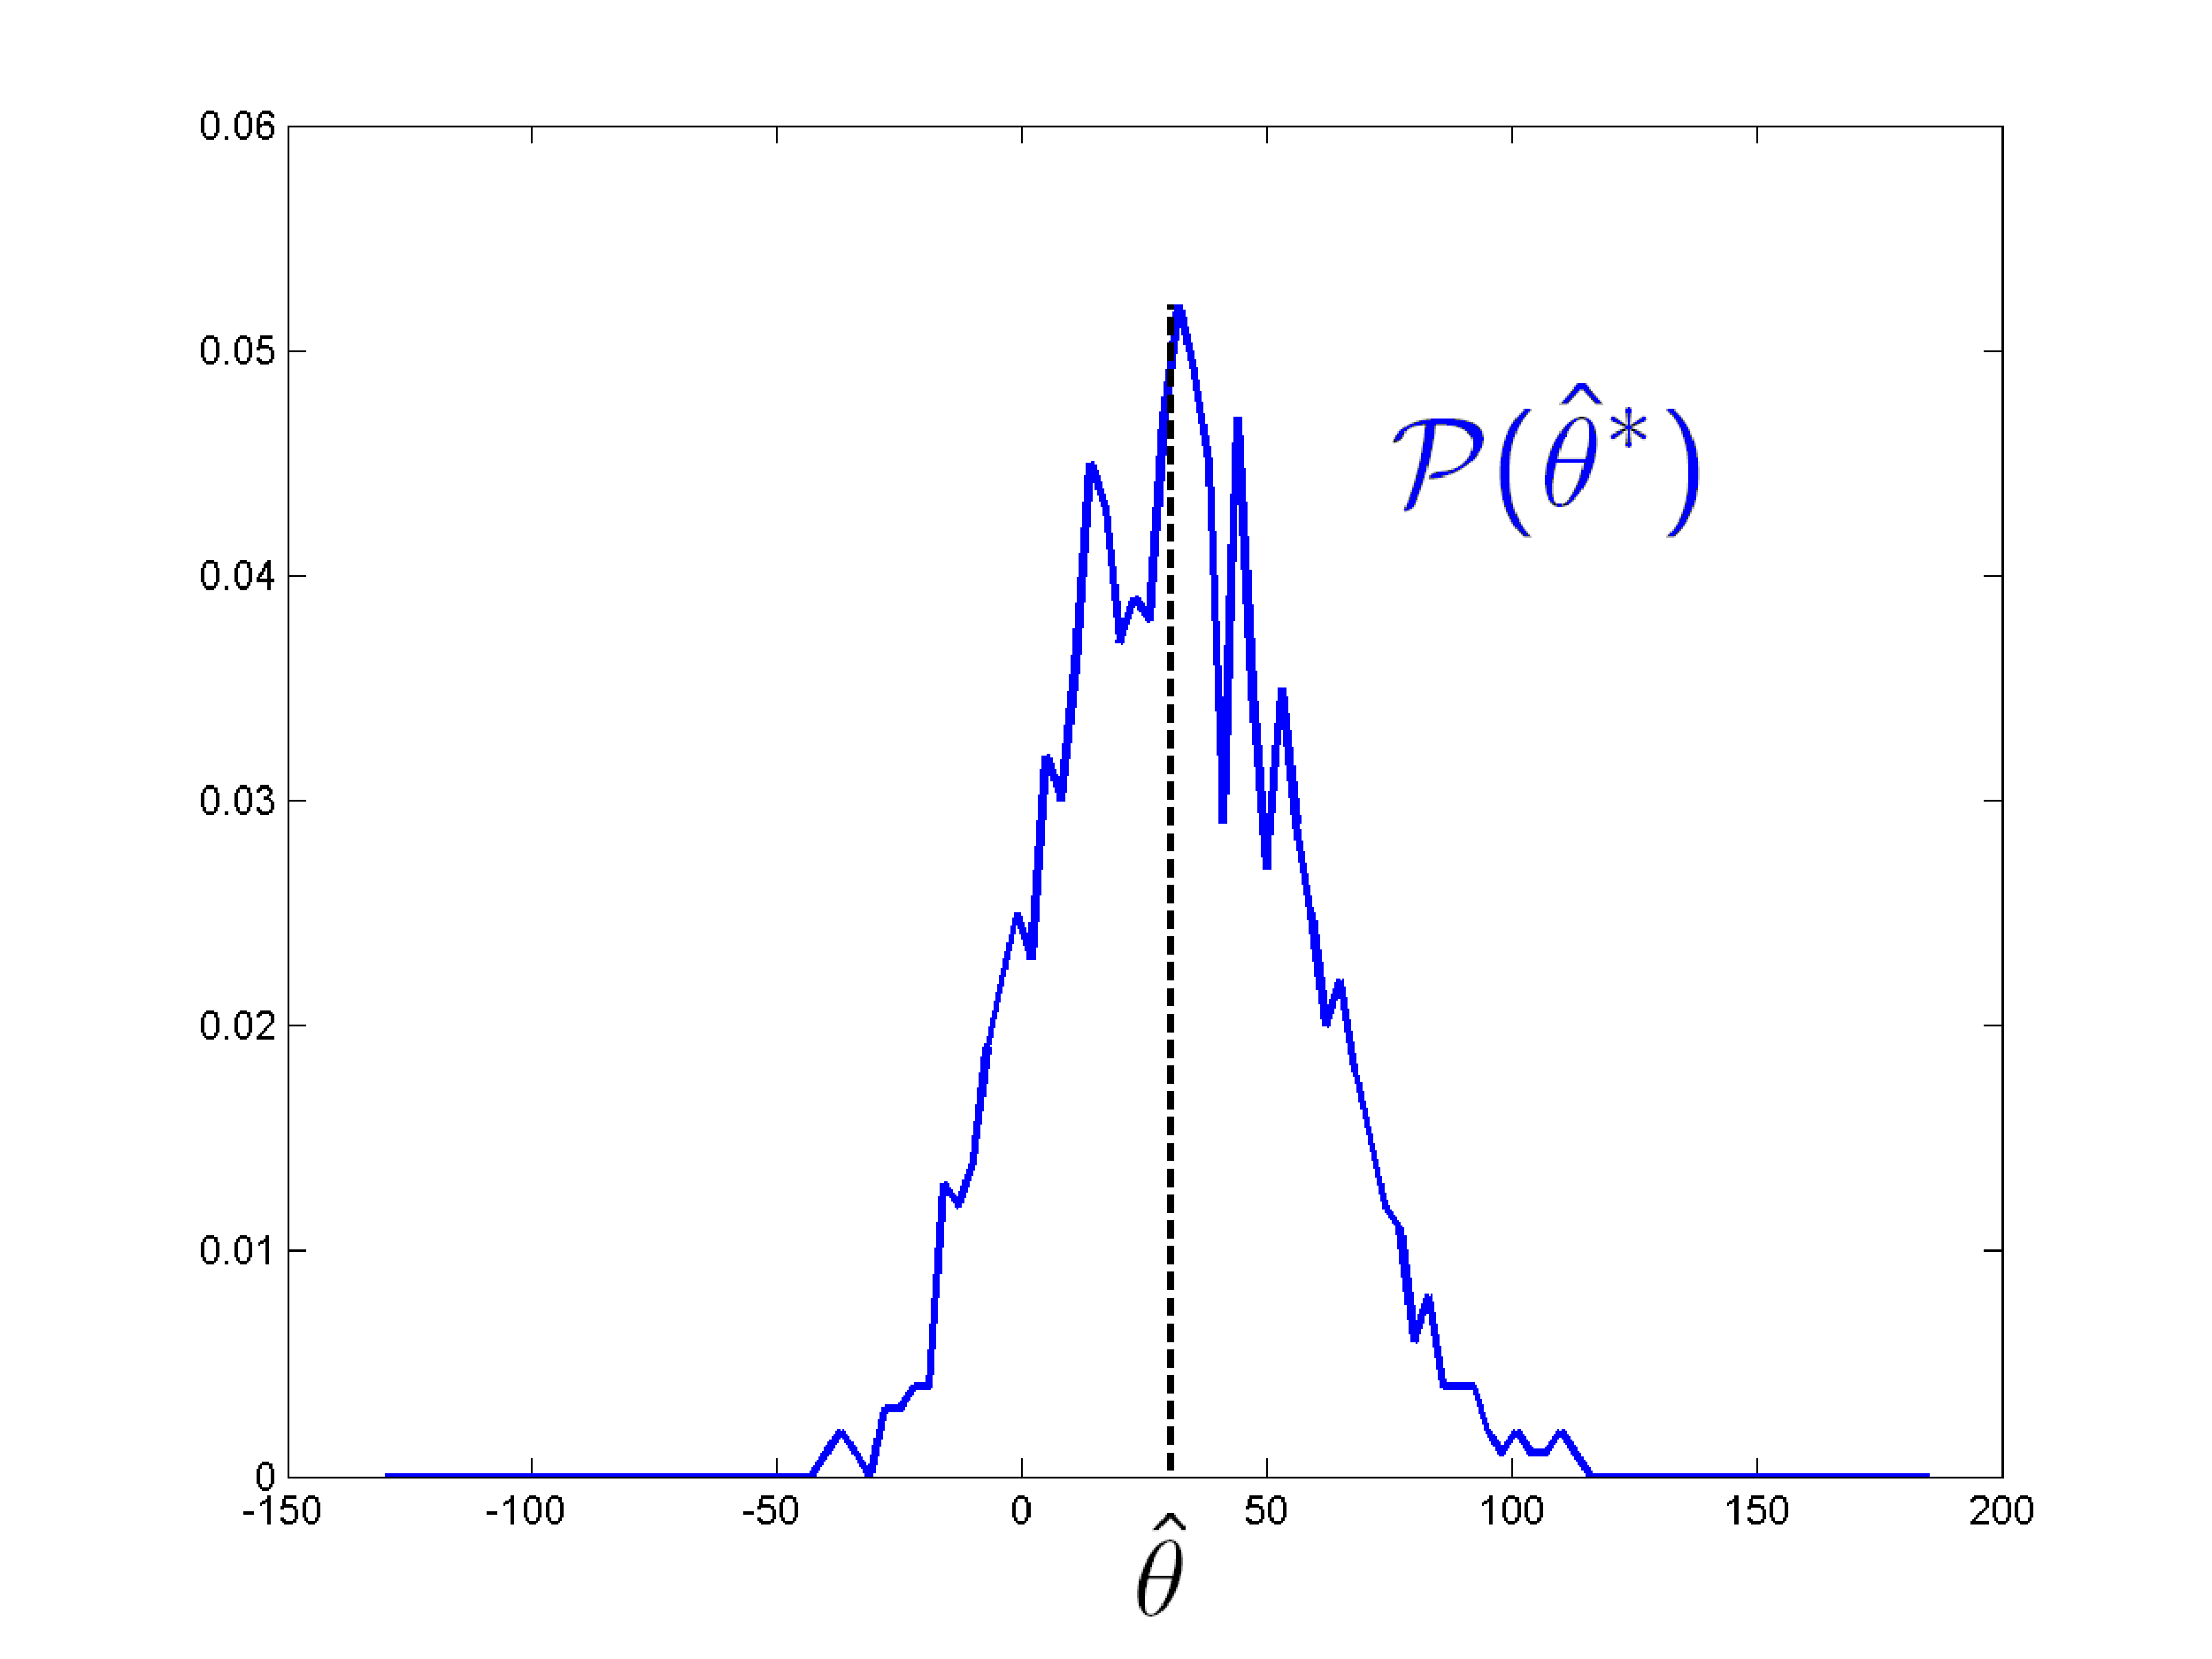
\includegraphics[scale=.2]{originalboot}
\caption{P.d.f. $\mathcal{P}(\hat{\theta}^{*})$ (histogram)  of the replication $\hat{\theta}^{*}$ ( $\hat{\theta}=30.63$
and $\hat{se}_B=26.85$).}
\end{figure}

}
%%%%%%%%%%%%%%%%%%%%%%%%%%%%%%%%%%%%%%%%%%%%%%%%%%
%\frame
%{
%\frametitle{Example on the mouse data}

%\begin{figure}
%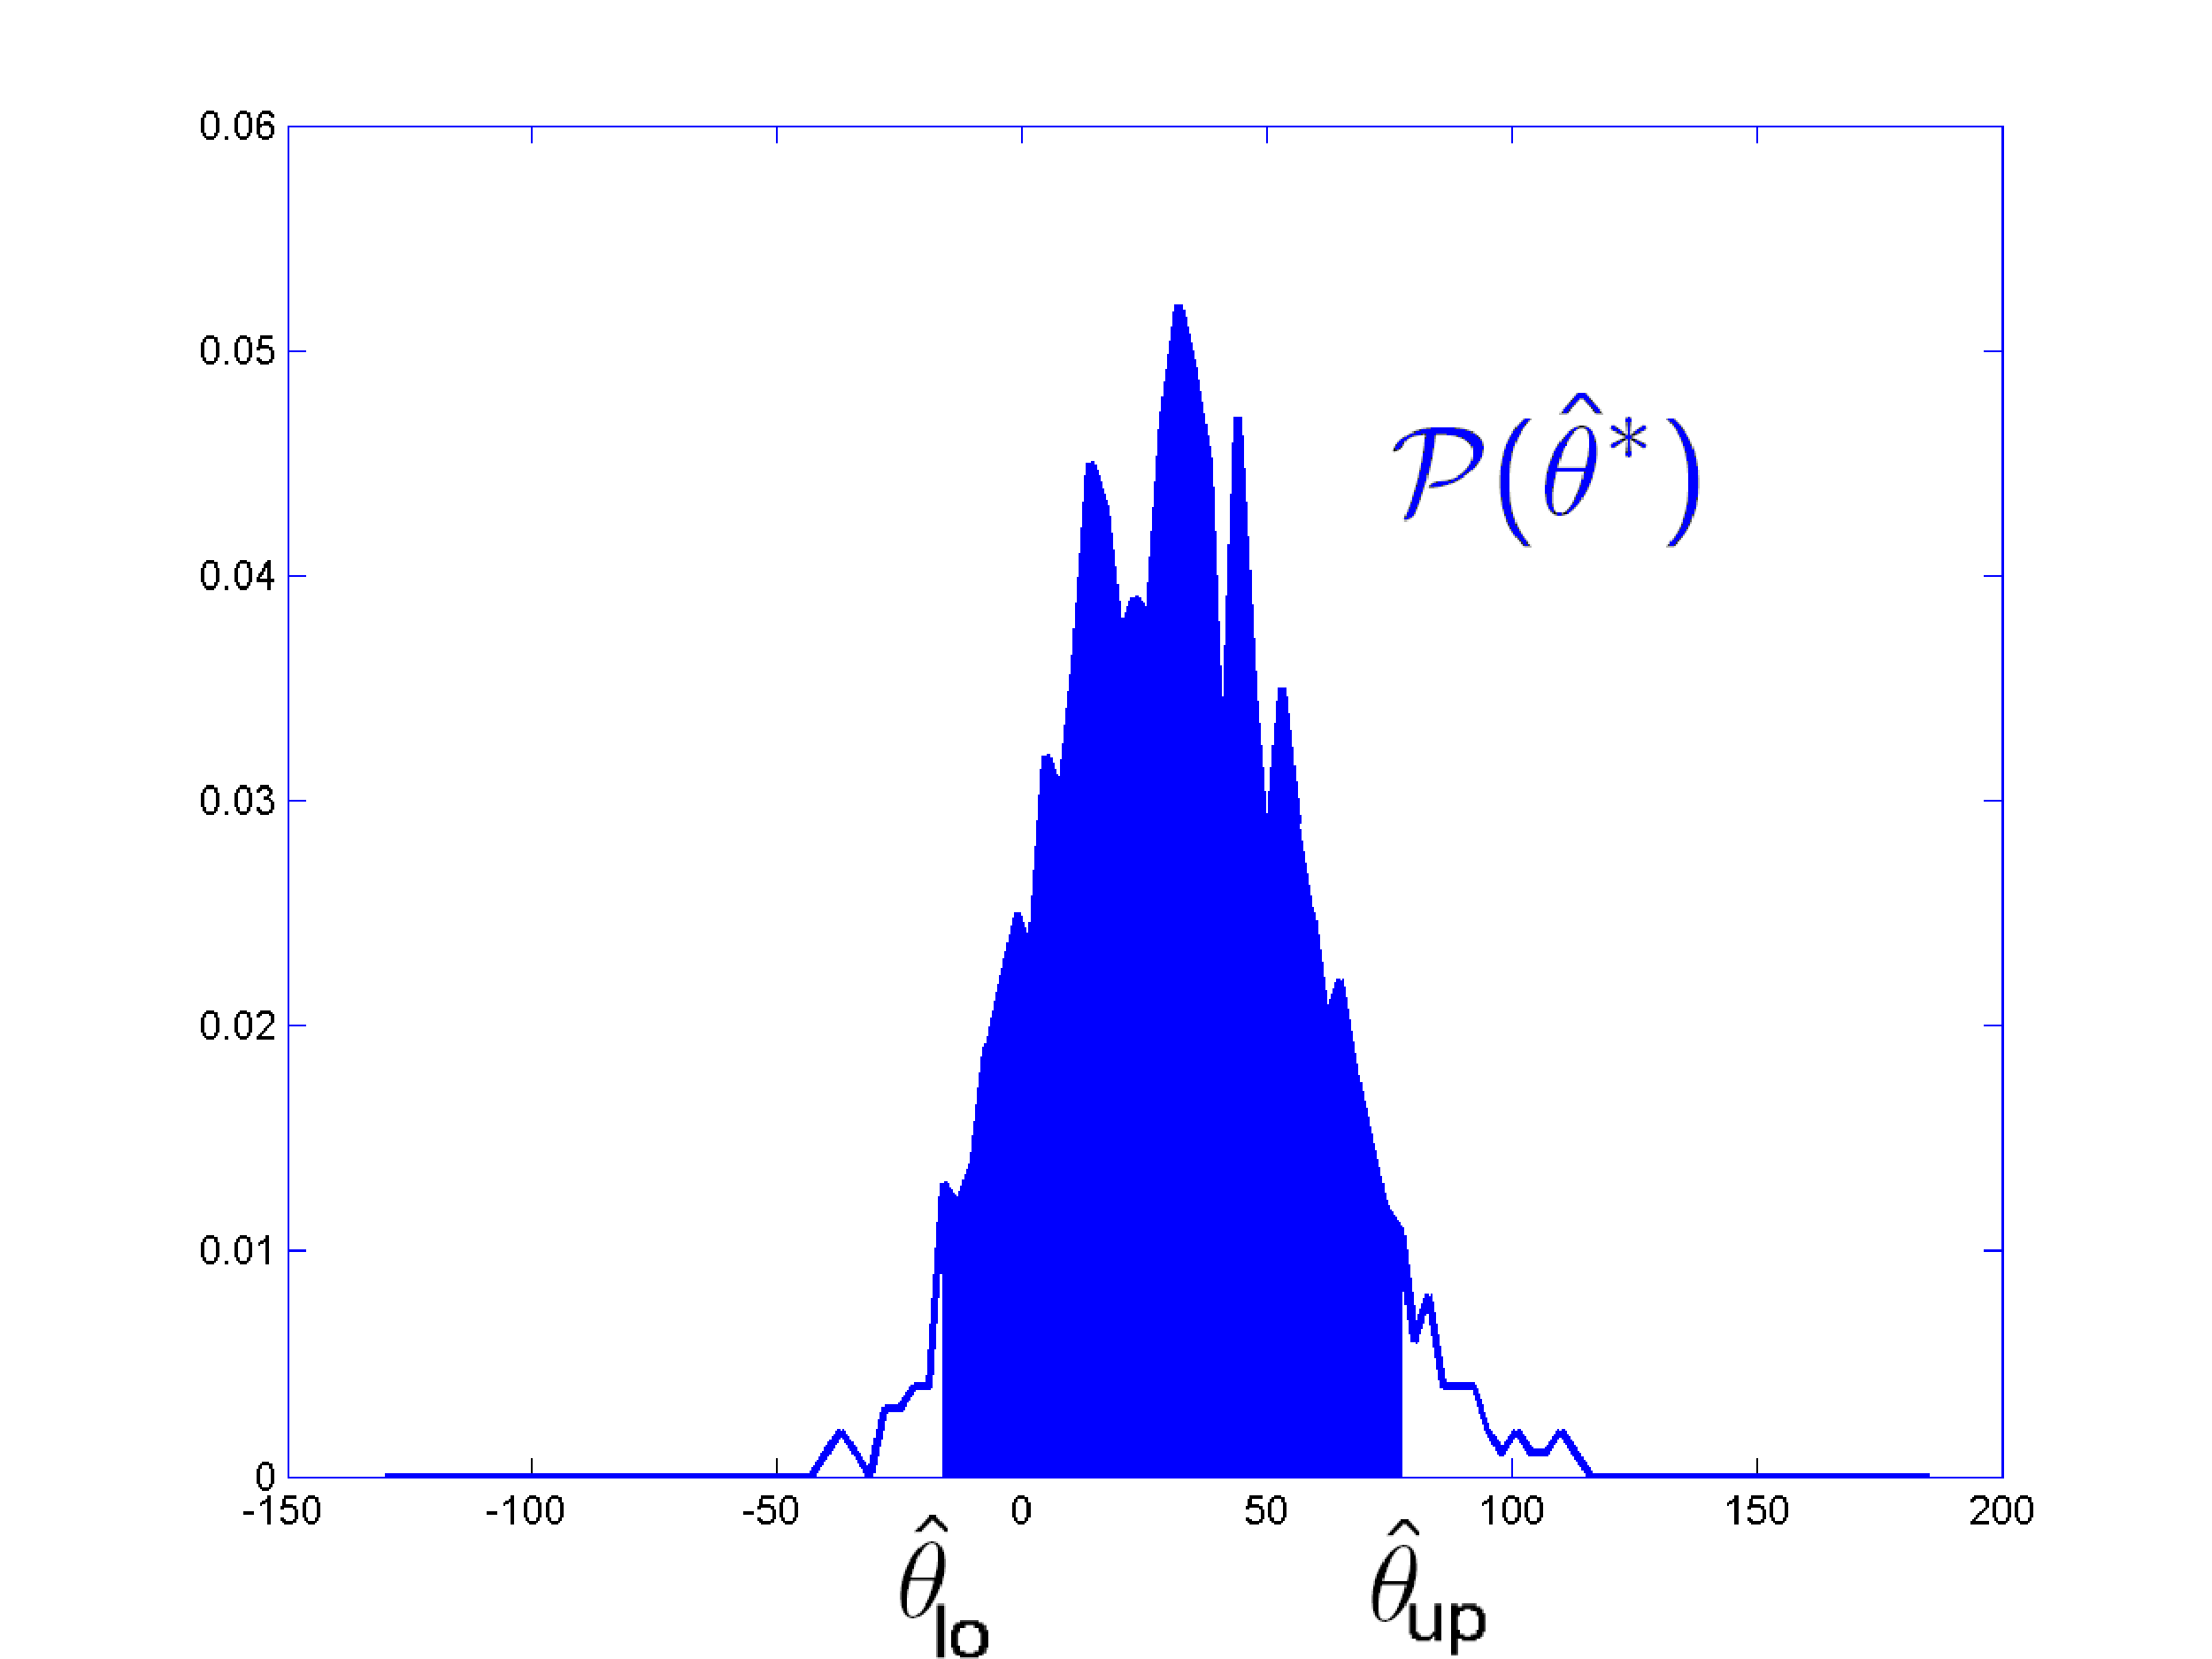
\includegraphics[scale=.2]{originalboot2}
%\caption{P.d.f. (histogram) of the replication $\hat{\theta}$ ($\mathcal{P}(\hat{\theta}^{*})$) with the 90 \% confidence interval defined by $\hat{\theta}_{lo}=\hat{\theta}-1.645*\hat{se}$ and $\hat{\theta}_{up}=\hat{\theta}+1.645*\hat{se}$. }
%\end{figure}
%}
\frame{
\frametitle{Introduction}

\begin{itemize}
\item Two sample problem : definitions

\

\item Parametric solution

\

\item Non parametric solution:

\

\begin{itemize}
\item permutation test

\

\item randomization test

\

\item bootstrap test
\end{itemize}
\end{itemize}
}
%%%%%%%%%%%%%%%%%%%%%%%%%%%%%%%%%%%%%%%%%%%%%%%%%%
\frame
{
\frametitle{The two sample problem}

Two independent random sample are observed $\mathbf{x}_{a}$ and $\mathbf{x}_{b}$ drawn from possibly different probability density functions:
$$
\begin{array}{l}
 f_{a}  \rightsquigarrow \mathbf{x}_a=\lbrace x_{a,1},\cdots, x_{a,n} \rbrace\\
\\
f_{b}  \rightsquigarrow \mathbf{x}_b=\lbrace x_{b,1},\cdots, x_{b,m} \rbrace
\end{array}
$$
\begin{definition}
The \alert{null hypothesis $\mathcal{H}_0$} assumes that there is no difference in between the density function $f_a=f_b$.
\end{definition}

}


%%%%%%%%%%%%%%%%%%%%%%%%%%%%%%%%%%%%%%%%%%%%%%%%
\frame
{
\frametitle{Hypothesis  test and Achieved significance level (ASL)}

\begin{definition}
A \alert{hypothesis test} is a way of deciding whether or not the data decisively reject the hypothesis $\mathcal{H}_0$. 
\end{definition}

\begin{definition}
The \alert{achieved significance level} of the test (ASL) is defined as:
$$
\begin{array}{ll}
\mathrm{ASL}&= \pmb{\mathcal{P}}(\hat{\theta}^{*}\geq \hat{\theta}|\mathcal{H}_0)\\
&\\
&=\int^{+\infty}_{\hat{\theta}} \mathcal{P}(\hat{\theta}^{*}|\mathcal{H}_0) \ d\hat{\theta}^{*}\\
\end{array}
$$ 
The smaller ASL, the stronger is the evidence of  $\mathcal{H}_0$ false. The notation star differentiates between  an hypothetical value $\hat{\theta}^{*}$ generated according to $\mathcal{H}_0$, and the actual observation $\hat{\theta}$.
\end{definition}
}
%%%%%%%%%%%%%%%%%%%%%%%%%%%%%%%%%%%%%%%%%%%%%%%%%%
\frame
{
\frametitle{Parametric test}

\begin{itemize}

\item A tradionnal way is to consider some hypotheses: $f_a \sim \mathcal{N}(\mu_a, \sigma^2)$ and $f_b \sim \mathcal{N}(\mu_b, \sigma^2)$, and the null hypothesis becomes $\mu_a=\mu_b$. 

\

\item Under $\mathcal{H}_{0}$, the statistic $\hat{\theta}=\overline{x}_a-\overline{x}_b$ can be modelled as a normal distribution with mean 0 and variance $\sigma^2_{\hat{\theta}}=\sigma^2 (\frac{1}{m}+\frac{1}{n})$. 

\

\item The ASL is then computed:
$$
\mathrm{ASL}= \int^{+\infty}_{\hat{\theta}} 
\frac{
e^{ \frac{- (\hat{\theta}^{*}-\hat{\theta} )^{2} } {2\sigma^2_{\hat{\theta}}  }}} {\sqrt{2\pi} \sigma_{\hat{\theta}}} \ 
d\hat{\theta}^{*}
$$

\end{itemize}
}
%%%%%%%%%%%%%%%%%%%%%%%%%%%%%%%%%%%%%%%%%%%%%%%%%%
\frame
{
\frametitle{Parametric test}

\begin{itemize}
\item $\sigma$ is unknown and has to be estimated from the data:
$$ 
\overline{\sigma}^2= \frac{\sum_{i=1}^{n} (x_{ai}-\overline{x}_{a})^2 +\sum_{i=1}^{m} (x_{bi}-\overline{x}_{b})^2} {m+n-2}
$$



\item For the mouse data $\mathrm{ASL}=.131$ : the null hypothesis cannot be rejected.

\

\item However, this (parametric) method relies on the hypotheses made while calculating the ASL.  

\end{itemize} 

}
%%%%%%%%%%%%%%%%%%%%%%%%%%%%%%%%%%%%%%%%%%%%%%%%%%
\frame
{
\frametitle{Permutation tests}

\begin{itemize}
\item \textit{Permutation tests} are a computer-intensive statistical technique that predates computers. 

\ 

\item This idea was introduced by R.A. Fisher in the 1930's.

\

\item The main application of permutation tests is the two-sample problem. 

\end{itemize}
}




%%%%%%%%%%%%%%%%%%%%%%%%%%%%%%%%%%%%%%%%%%%%%%%%%
\frame
{
\frametitle{Computation of the two sample permutation test statistic}

\begin{block}{}
Notation $m$ number of values in  observation $\mathbf{x}_{Treat}$, $n$ number of values in observation $\mathbf{x}_{Cont}$. 

\alert{If $\mathcal{H}_0$ is true, then:} 
\begin{enumerate}
\item We can combine the values from both observations in one of size $m+n=N$:  $\mathbf{x}=\lbrace \mathbf{x}_{Treat}, \mathbf{x}_{Cont}\rbrace$.

\

\item Take a subsample $\mathbf{x}_{Treat}^{*}$ from $\mathbf{x}$ of size $m$. The remaining $n$ values constitute the subsample $\mathbf{x}_{Cont}^{*}$.

\

\item Compute the replication $\overline{x}^{*}_{Treat}$ and $\overline{x}^{*}_{Cont}$ on $\mathbf{x}_{Treat}^{*}$ and $\mathbf{x}_{Cont}^{*}$ respectively.

\

\item Compute the replication of the difference $\hat{\theta}^{*}=\overline{x}^{*}_{Treat}-\overline{x}^{*}_{Cont}$.
\end{enumerate}
\end{block}
}
%%%%%%%%%%%%%%%%%%%%%%%%%%%%%%%%%%%%%%%%%%%%%%%%%
\frame
{
\frametitle{Example on the mouse data}

\begin{figure}[!h]
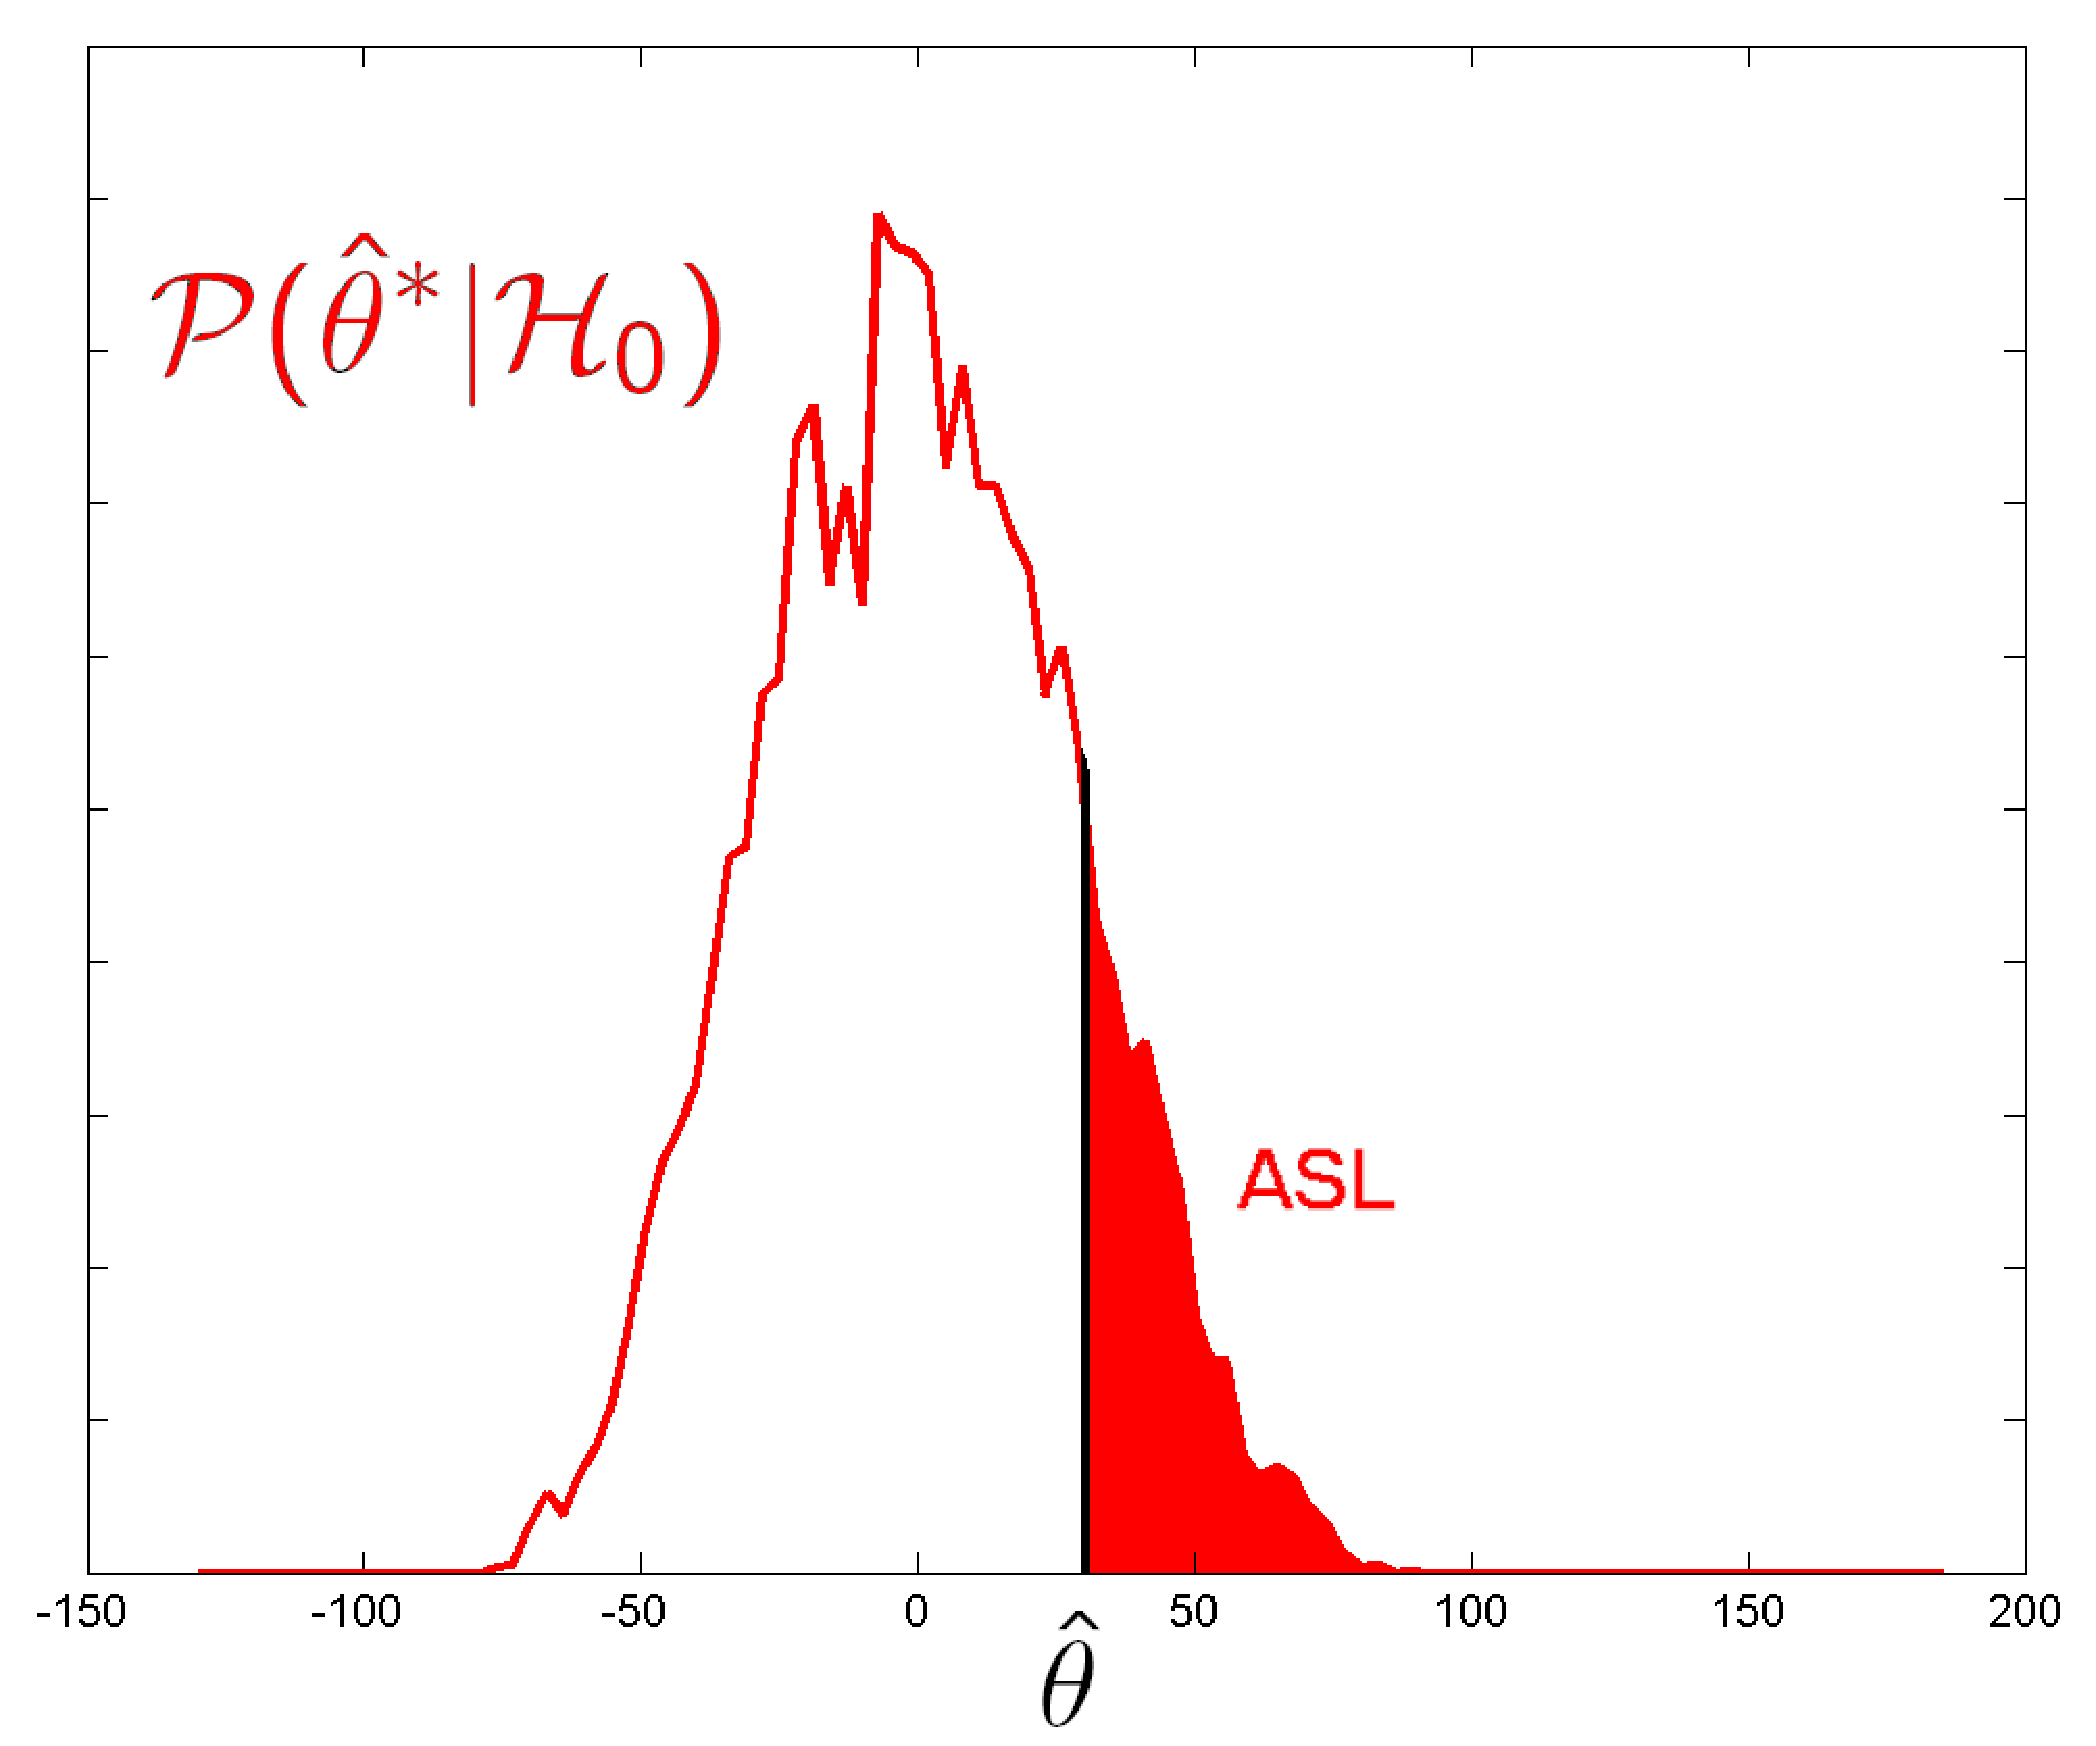
\includegraphics[scale=.15]{perm}
\caption{Histogram of the permutation replications $\mathcal{P}(\hat{\theta}^{*}|\mathcal{H}_{0})$. ASL is the red surface ($\mathrm{ASL}_{perm}=0.14$).}
\end{figure}

\begin{block}{}
\small{If the original difference $\hat{\theta}=d=\overline{x}_{Treat}-\overline{x}_{Cont}$ falls outside the 95\% of the distribution of the permutation replication  (i.e. $\mathrm{ASL}_{perm}<0.05$), then the null hypothesis is rejected.}  
\end{block}
}
%%%%%%%%%%%%%%%%%%%%%%%%%%%%%%%%%%%%%%%%%%%%%%%%%
\frame
{
\frametitle{Computation of the two sample permutation test statistic}

\begin{beamercolorbox}[wd=\linewidth, rounded=true,shadow=true]{postit}

\begin{enumerate}
\item $\mathbf{x}=\lbrace \mathbf{x}_a;\mathbf{x}_b \rbrace$ of size $n+m=N$. 

\

\item Compute  all  :


\begin{itemize}
\item $
\left(
\begin{array}{l}
 N\\ 
 n \\
 \end{array}
\right)
$ permutation samples $\mathbf{x}^{*}$. Select the $n$ first values to define $\mathbf{x}^{*}_a$ and the last $m$ ones to define $\mathbf{x}^{*}_b$

\ 

\item  $
\left(
\begin{array}{l}
 N\\ 
 n \\
 \end{array}
\right)
$ replications $\hat{\theta}^{*}(b)=\overline{x}_{a}^{*}-\overline{x}_{b}^{*}$
\end{itemize}

\

\item Approximate $\mathrm{ASL}_{perm}$ by:
$$
\widehat{\mathrm{ASL}}_{perm}= \frac{\# \lbrace \hat{\theta}^{*} \geq \hat{\theta} \rbrace}{\left(
\begin{array}{l}
 N\\ 
 n \\
 \end{array}
\right)}
$$
\end{enumerate}

\end{beamercolorbox}
}
%%%%%%%%%%%%%%%%%%%%%%%%%%%%%%%%%%%%%%%%%%%%%%%%
\frame{
\frametitle{Remark on the permutation test}
\begin{itemize}
\item The histogram of the \alert{permutation replications} $\hat{\theta}^{*}$ approximates $\mathcal{P}(\hat{\theta}^*|\mathcal{H}_0)$.

\

\item The resamples are not really permutations but more combinations. 
  
\

\item $\left(
\begin{array}{l}
 N\\ 
 n \\
 \end{array}
\right)$  can be huge so in practice, ASL$_{perm}$ is approximated by Monte Carlo methods. 

\end{itemize}
}
%%%%%%%%%%%%%%%%%%%%%%%%%%%%%%%%%%%%%%%%%%%%%%%%%
\frame
{
\frametitle{Computation of the two sample randomization test statistic}

\begin{beamercolorbox}[wd=\linewidth, rounded=true,shadow=true]{postit}

\begin{enumerate}
\item $\mathbf{x}=\lbrace \mathbf{x}_a;\mathbf{x}_b \rbrace$ of size $n+m=N$. 

\

\item Compute $B$ times:


\begin{itemize}
\item Randomly selected permutation samples $\mathbf{x}^{*}$. Select the $n$ first values to define $\mathbf{x}^{*}_a$ and the last $m$ ones to define $\mathbf{x}^{*}_b$

\ 

\item Compute the replications $\hat{\theta}^{*}(b)=\overline{x}_{a}^{*}-\overline{x}_{b}^{*}$
\end{itemize}

\

\item Approximate $\mathrm{ASL}_{perm}$ by:
$$
\widehat{\mathrm{ASL}}_{perm}= \frac{\# \lbrace \hat{\theta}^{*} \geq \hat{\theta} \rbrace}{B}
$$
\end{enumerate}

\end{beamercolorbox}
}
%%%%%%%%%%%%%%%%%%%%%%%%%%%%%%%%%%%%%%%%%%%%%%
\frame
{
\frametitle{Remarks}

\begin{figure}[!h]
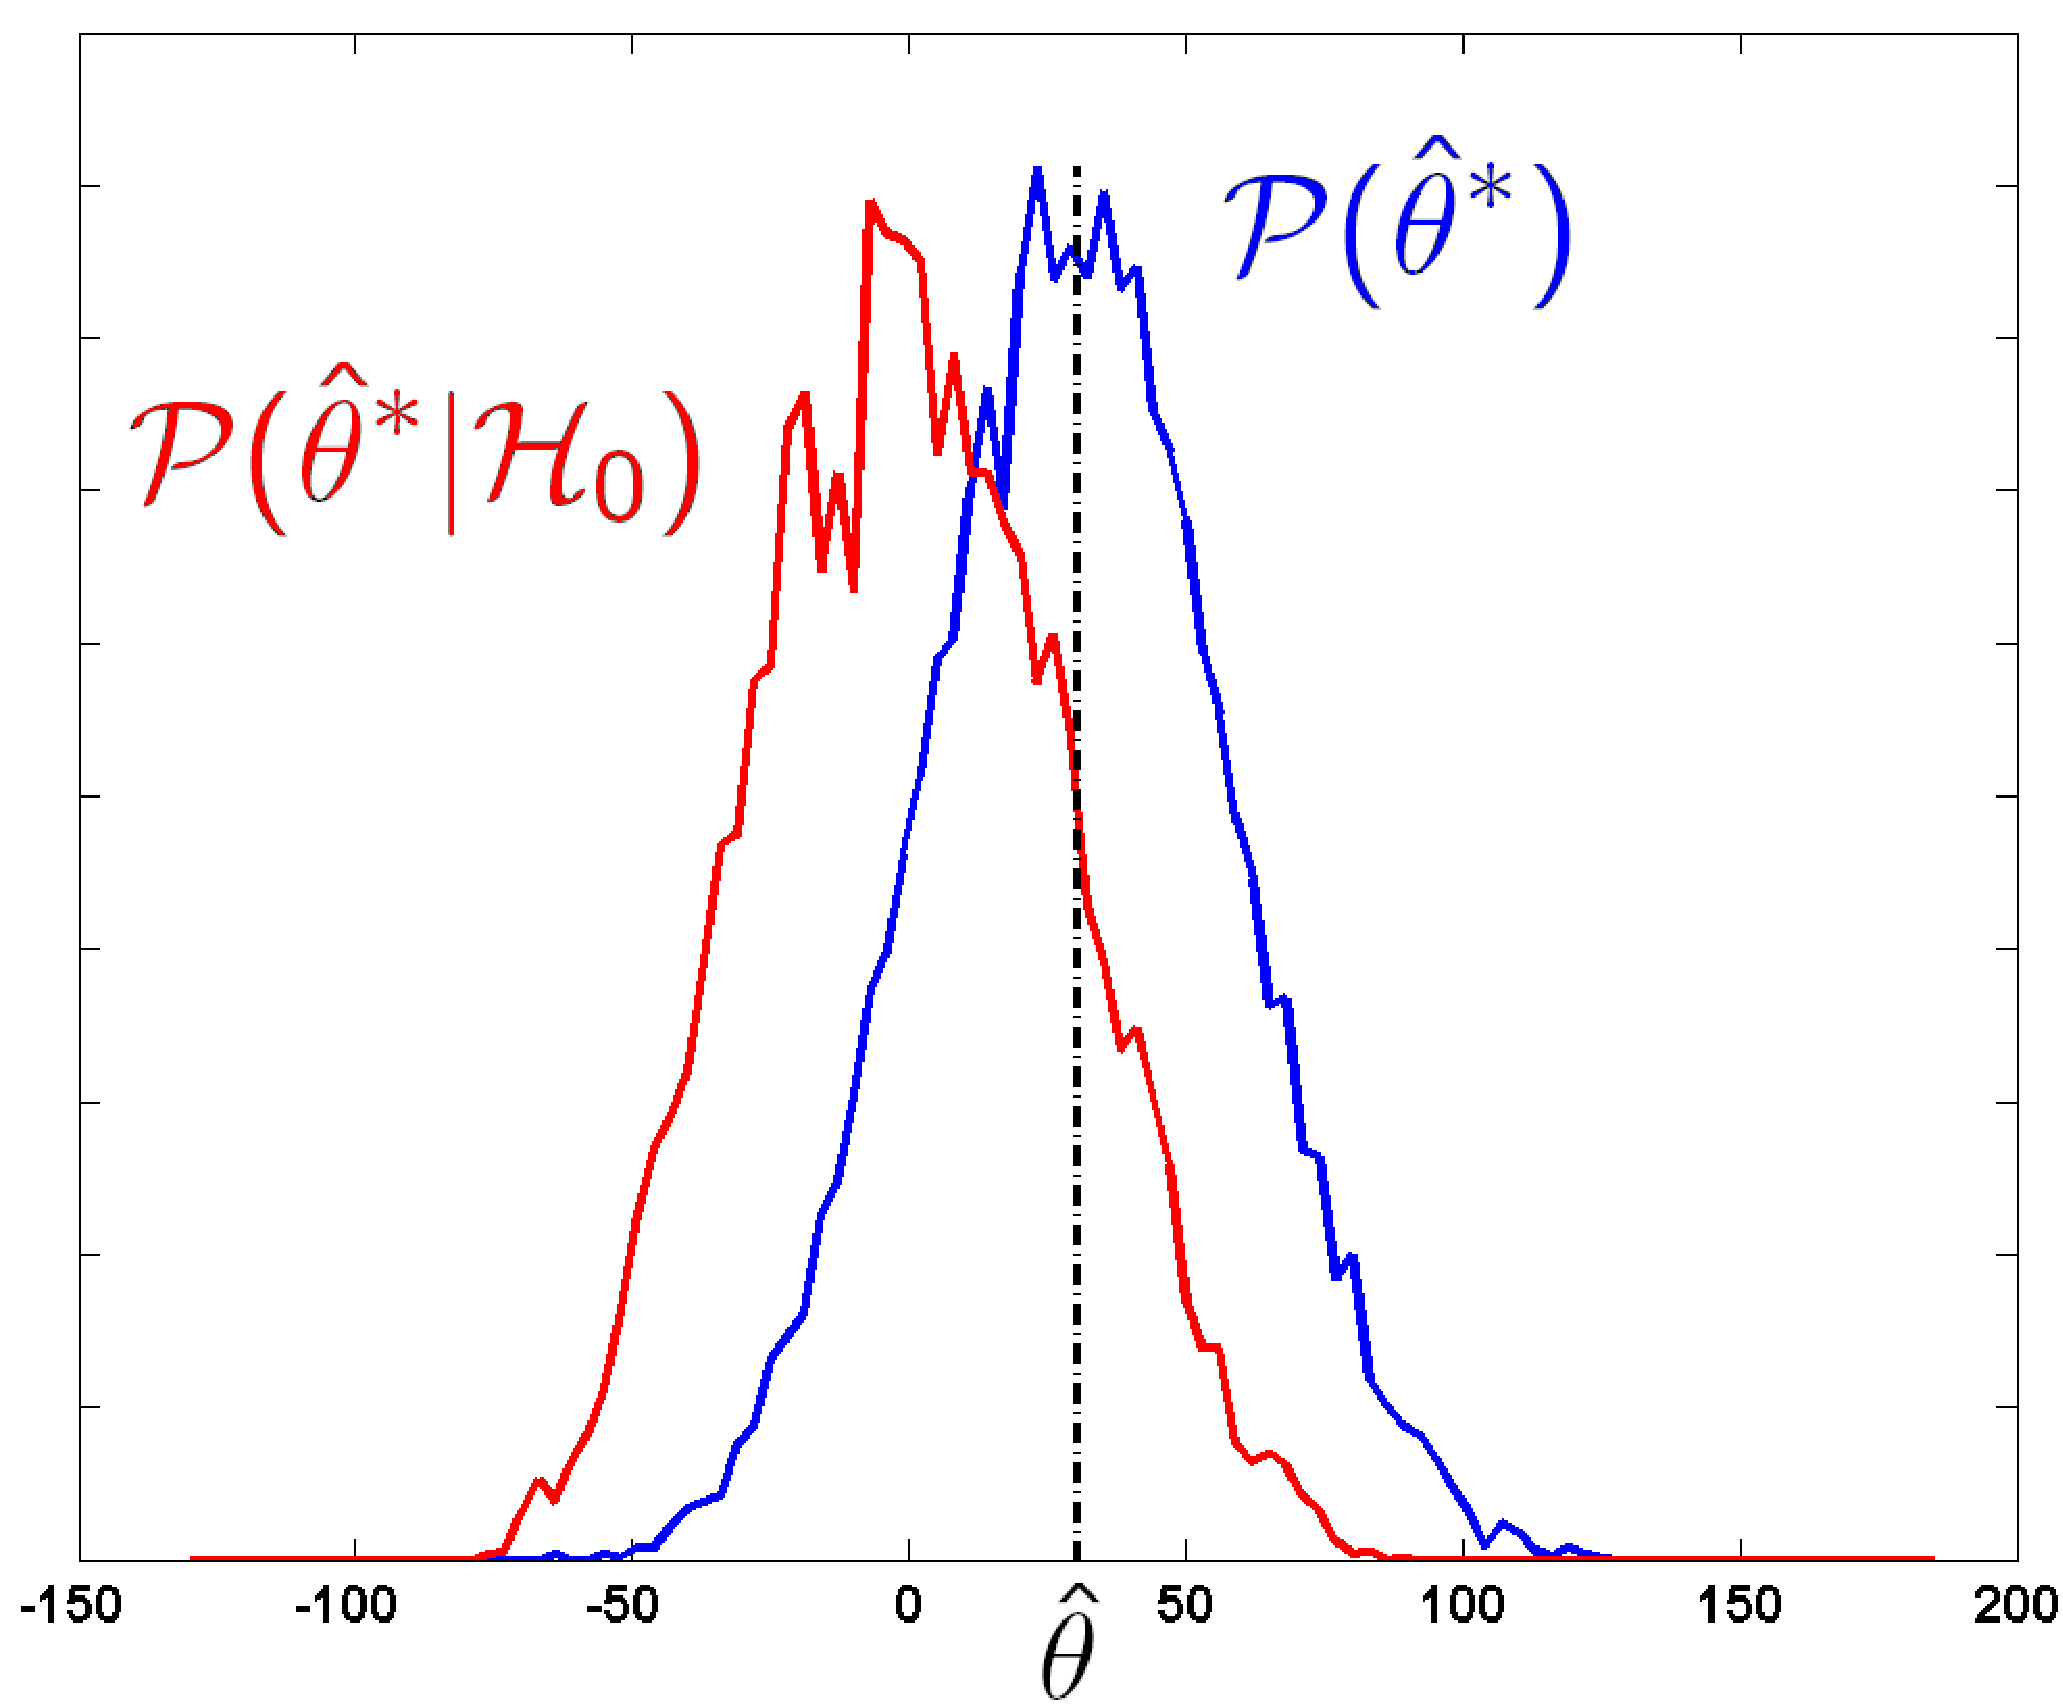
\includegraphics[scale=.2]{permboot}
\caption{Histograms of the bootstrap replications $\mathcal{P}(\hat{\theta}^{*})$ (blue), and the permutation replications $\mathcal{P}(\hat{\theta}^{*}|\mathcal{H}_{0})$ (red). }
\end{figure}
}
%%%%%%%%%%%%%%%%%%%%%%%%%%%%%%%%%%%%%%%%%%%%%%%%%
\frame
{
\frametitle{Remarks} 

\begin{itemize}

\item Permutation replications are computed  without replacement.

\

\item The  distribution of permutation replications approximates $\mathcal{P}(\theta^{*}|\mathcal{H}_0)$.

\

\item The bootstrap replications presented in the introduction are computed on resamples with replacements. The distribution of those bootstrap replications defines $\mathcal{P}(\theta^{*})$. 

\

\item Is there a way to get $\mathcal{P}(\theta^{*}|\mathcal{H}_0)$ using a bootstrap method ?

\end{itemize}

}


%%%%%%%%%%%%%%%%%%%%%%%%%%%%%%%%%%%%%%%%%%%%%%%%%
\frame
{
\frametitle{Computation of the two sample bootstrap test statistics}

\begin{beamercolorbox}[wd=\linewidth, rounded=true,shadow=true]{postit}

\begin{enumerate}
\item $\mathbf{x}=\lbrace \mathbf{x}_a;\mathbf{x}_b \rbrace$ of size $n+m=N$. 

\
\item Compute $B$ times:

\begin{itemize}
\item Bootstrap samples from  $\mathbf{x}$. Select the $n$ first values to define $\mathbf{x}^{*}_a$ and the last $m$ ones to define $\mathbf{x}^{*}_b$.

\

\item Compute the replications $\hat{\theta}^{*}(b)=\overline{x}_{a}^{*}-\overline{x}_{b}^{*}$
\end{itemize}

\item Approximate $\mathrm{ASL}_{boot}$ by:
$$
\widehat{\mathrm{ASL}}_{boot}= \frac{\# \lbrace \hat{\theta}^{*}(b) \geq \hat{\theta} \rbrace}{B}
$$
\end{enumerate}

\end{beamercolorbox}

}
%%%%%%%%%%%%%%%%%%%%%%%%%%%%%%%%%%%%%%%%%%%%%%%%%
\frame
{
\frametitle{Example on the mouse data}

\begin{figure}[!h]
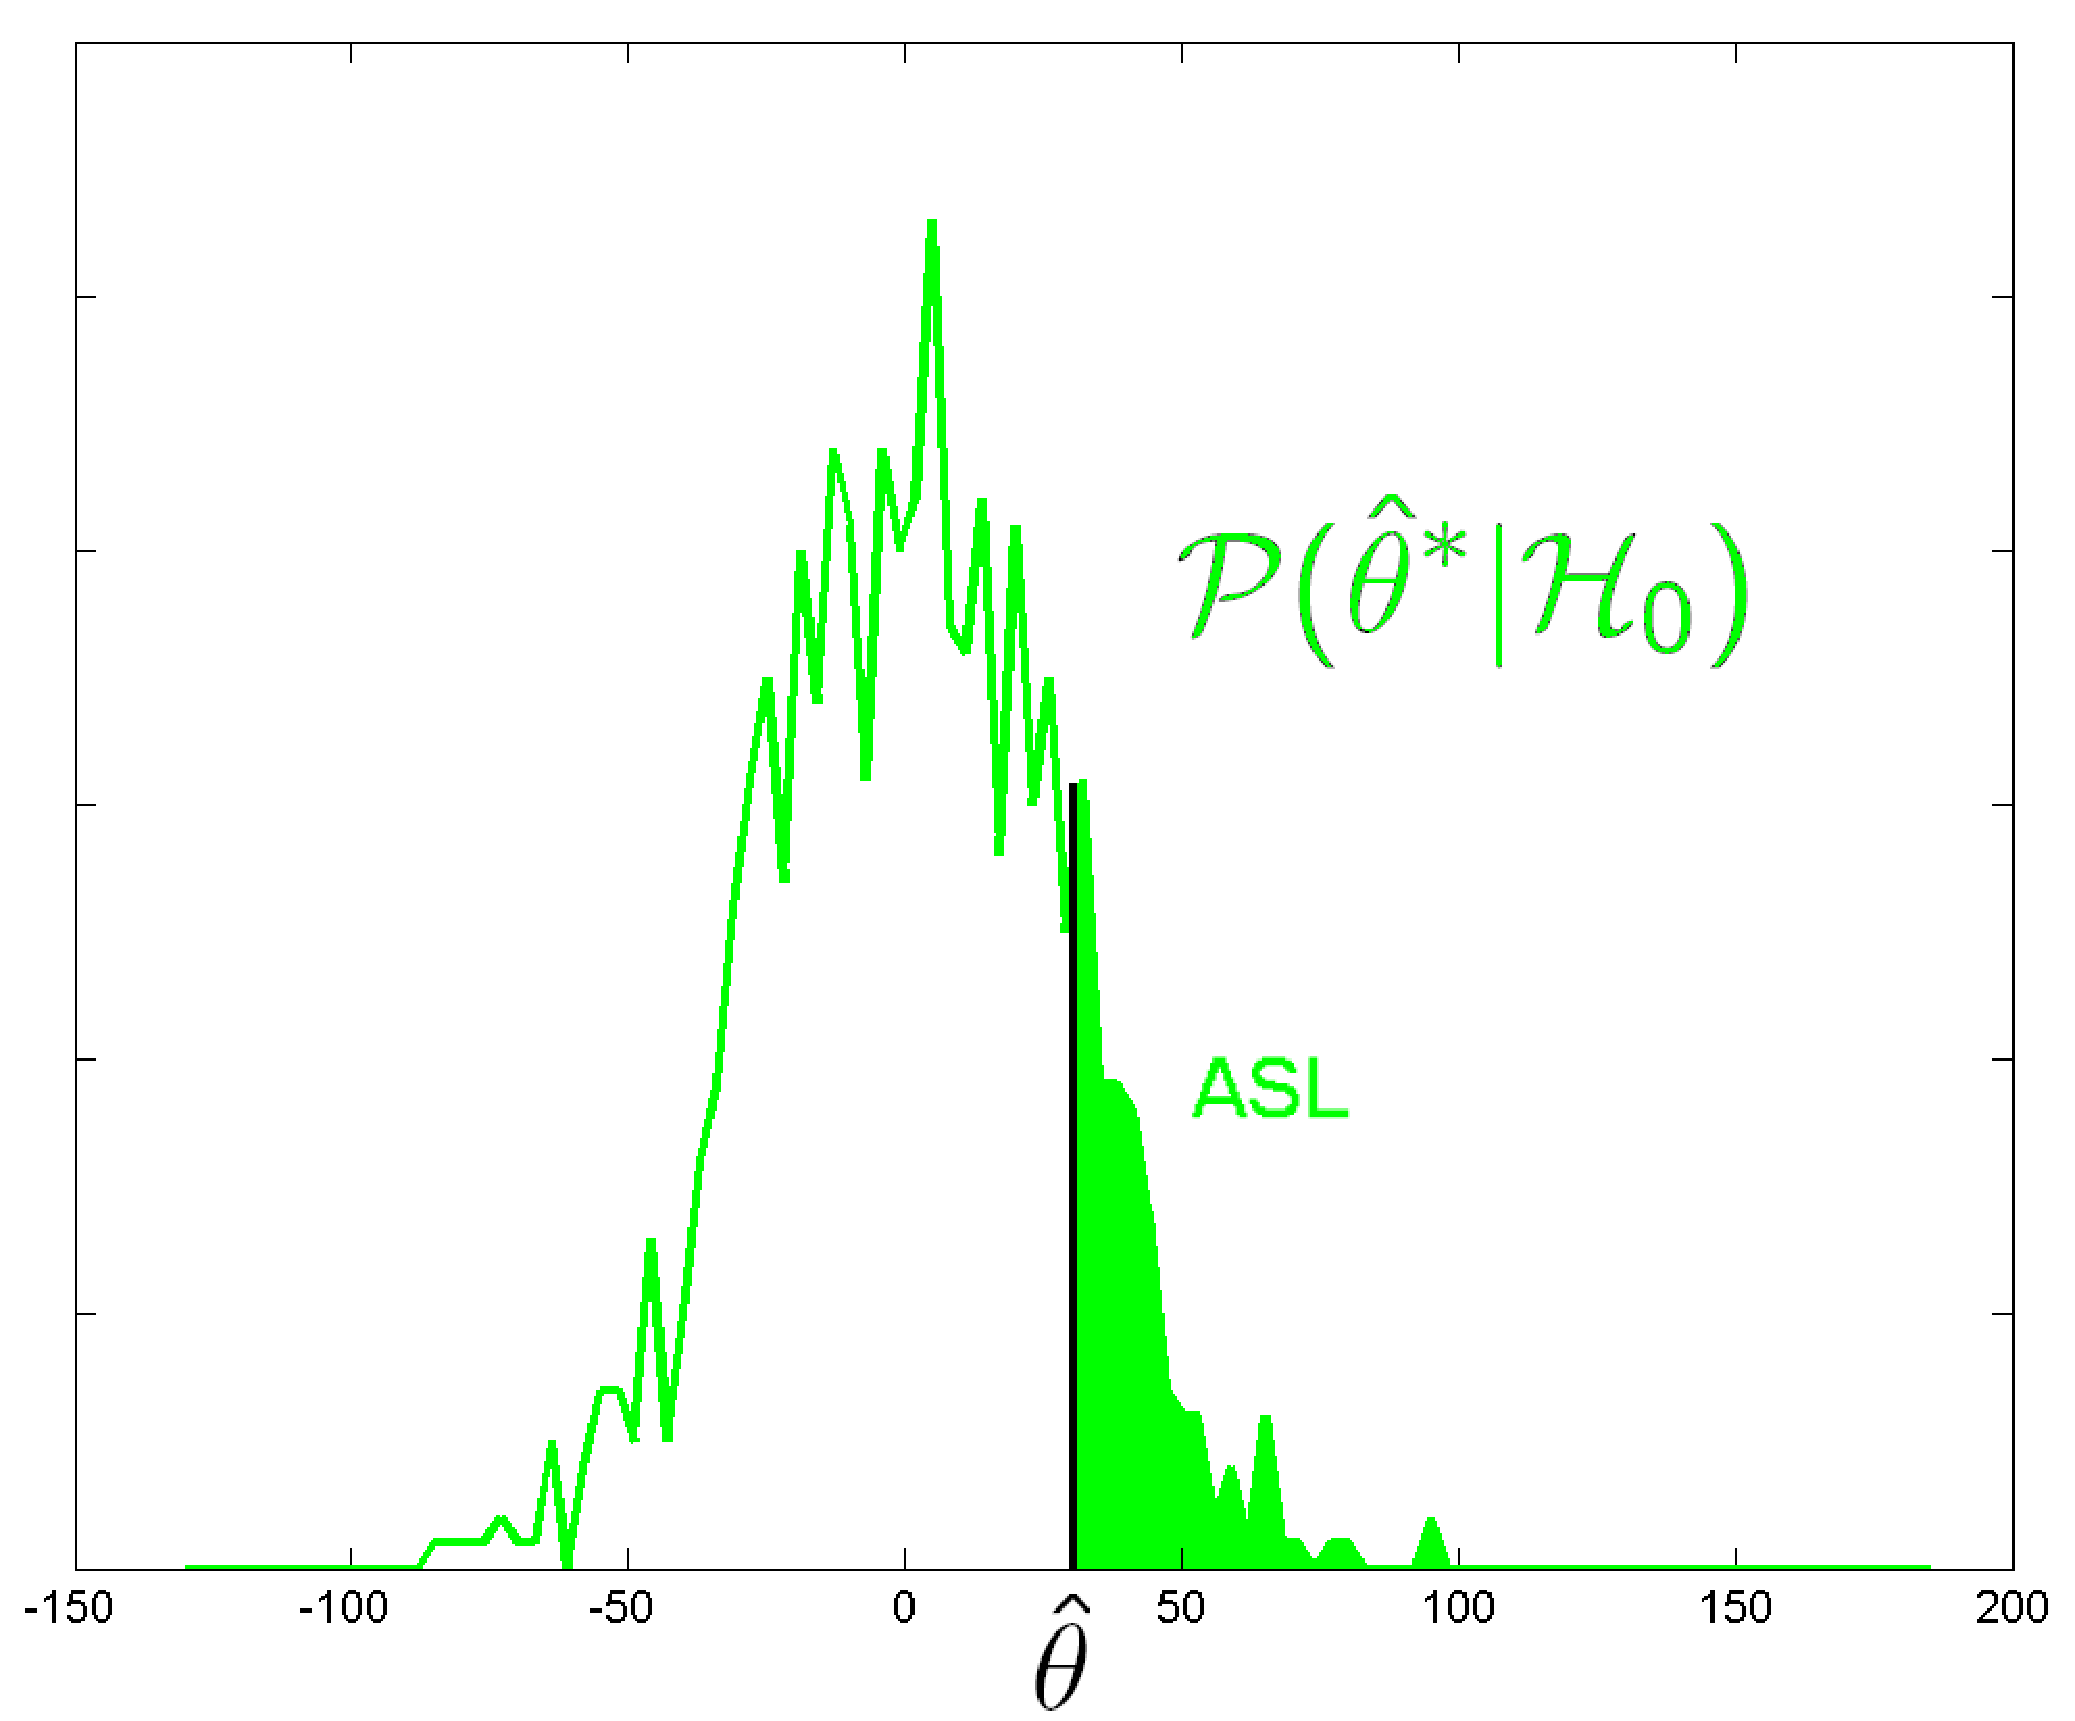
\includegraphics[scale=.2]{boot2sample}
\caption{Histogram of the \alert{bootstrap replications in the two sample test $\mathcal{P}(\hat{\theta}^{*}|\mathcal{H}_{0})$}. ASL is the green surface ($\mathrm{ASL}_{boot}=0.13$).}
\end{figure}

}

%%%%%%%%%%%%%%%%%%%%%%%%%%%%%%%%%%%%%%%%%%%%%%%%
\frame
{
\frametitle{Relationship between the permutation test and the bootstrap test}

\begin{itemize}
\item Very similar results in between the permutation test and the bootstrap test.


\


\item $\mathrm{ASL}_{perm}$ is the exact probability.   

\

\item $\mathrm{ASL}_{boot}$ is not an exact probability but is guaranteed to be accurate as an estimate of the ASL, as the sample size goes to infinity.

\

\item In the two-sample problem, the permutation test can  only test the null hypothesis $f_a=f_b$ while the bootstrap can perform other hypothesis testing.  


\end{itemize}

}




%%%%%%%%%%%%%%%%%%%%%%%%%%%%%%%%%%%%%%%%%%%%%%%%

\frame
{
\frametitle{Summary}

\begin{itemize}

\item Hypothesis testing has been introduced, involving the computation of a probability ASL

\

\item Permutation, Randomization  and bootstrap tests have been introduced as alternative to parametric tests.

\

\item Again the main difference in between those nonparametric tests, is the way the resamples are computed (with or without replacements).

\end{itemize}


}


%%%%%%%%%%%%%%%%%%%%
\section{Cross-validation}
\frame{
\frametitle{Introduction to resampling methods}
\begin{itemize}
\item Definitions and Problems
\item Non-Parametric Bootstrap
\item Parametric Bootstrap
\item Jackknife
\item Permutation tests
\item \textbf{Cross-validation}
\end{itemize}
}

%%%%%%%%%%%%%%%%%%%%%%%%%%%%%%%%%%%%%%%%%%%%%%%%%%%%%%%%%%%%%
\frame{
\frametitle{Type of resampling}

\begin{itemize}

\item  \textbf{Randomization exact test} (or permutation test) developed by R. A. Fisher (1935/1960), the founder of classical statistical testing.

\

 \item  \textbf{Jackknife} invented by Maurice Quenouille (1949) and later developed by John W. Tukey (1958). 
% first purpose of Jackknife is to detect outliers

\

 \item \textbf{Bootstrap}  invented by Bradley Efron (1979, 1981, 1982) and further developed by Efron and Tibshirani (1993). 

\

 \item \textbf{Cross-validation} 

\end{itemize}
}
%%%%%%%%%%%%%%%%%%%%%%%%%%%%%%%%%%%%%%%%%%%%%%%%%%%%%%%%%%%%%%%
\frame{
\frametitle{Resampling}

\begin{definition}
\alert{Resampling} means that the inference is based upon repeated sampling within the same sample.
Resampling is tied to the Monte Carlo simulation. Some may distinguish both in that resampling consider all possible replications (permutation test, jackknife) and the Monte-Carlo sampling restrict the resampling to a certain number of replications (bootstrap, randomisation test). 
\end{definition}

Another difference in between resampling methods  is  the nature of the  resamples: computed with or without replacement.


}
%%%%%%%%%%%%%%%%%%%%%%%%%%%%%%%%%%%%%%%%%%%%%%%%%%%%%%%%%%%%%%%
\frame{
\frametitle{Introduction to cross-validation}

\begin{itemize}
\item \textbf{Cross-validation} was proposed by Kurtz (1948-simple cross-validation) , extended by Mosier (1951-double cross-validation) and  by Krus and Fuller  (1982-  multicross-validation).

\

\item The original objective of cross-validation is to verify replicability of results.

\

\item Similarly with hypothesis testing, the goal is to find out if the result is replicable or just a matter of random. 


\end{itemize}


}
%%%%%%%%%%%%%%%%%%%%%%%%%%%%%%%%%%%%%%%%%%%%%%%%%%%%%%%%%%%%%%%
\frame{
\frametitle{prediction error}

\begin{definition}
A \alert{prediction error} measures how well a model predicts the response value of a future observation. It is often used for model selection.

It is defined as:
\begin{itemize}
\item the expected square difference between a future response and the prediction from the model in regression models:
$$
\mathbb{E}(y-\hat{y})
$$
\item the probability of incorrect classification in classification problem: 
$$
\pmb{\mathcal{P}}(y \neq \hat{y})
$$
\end{itemize}
\end{definition}
}
%%%%%%%%%%%%%%%%%%%%%%%%%%%%%%%%%%%%%%%%%%%%%%%%%%%%%%%%%%%%%%%
\frame{
\frametitle{The linear regression model}
\begin{itemize}
\item We have a set of (2-dimensional) points $z =\lbrace (x_i,y_i) \rbrace_{i=1,\cdots,n}$. 
\item An unknow relation is linking $y_i$ to $x_i$ such as:
$$
\begin{array}{ll}
y_i&=\beta(x_i)+\epsilon_{i}\\
&\\
&=\sum_{q=0}^{p} \beta_q \ x_i^q+\epsilon_{i}\\
\end{array} 
$$
\item The error terms  $\epsilon_{i}$ are assumed to be random sample from a random distribution having expectation 0 and variance $\sigma^2$.


\end{itemize}



}
%%%%%%%%%%%%%%%%%%%%%%%%%%%%%%%%%%%%%%%%%%%%%%%%%%%%%%%%%
\frame{
\frametitle{The Model Selection Problem}

\begin{figure}[!h]
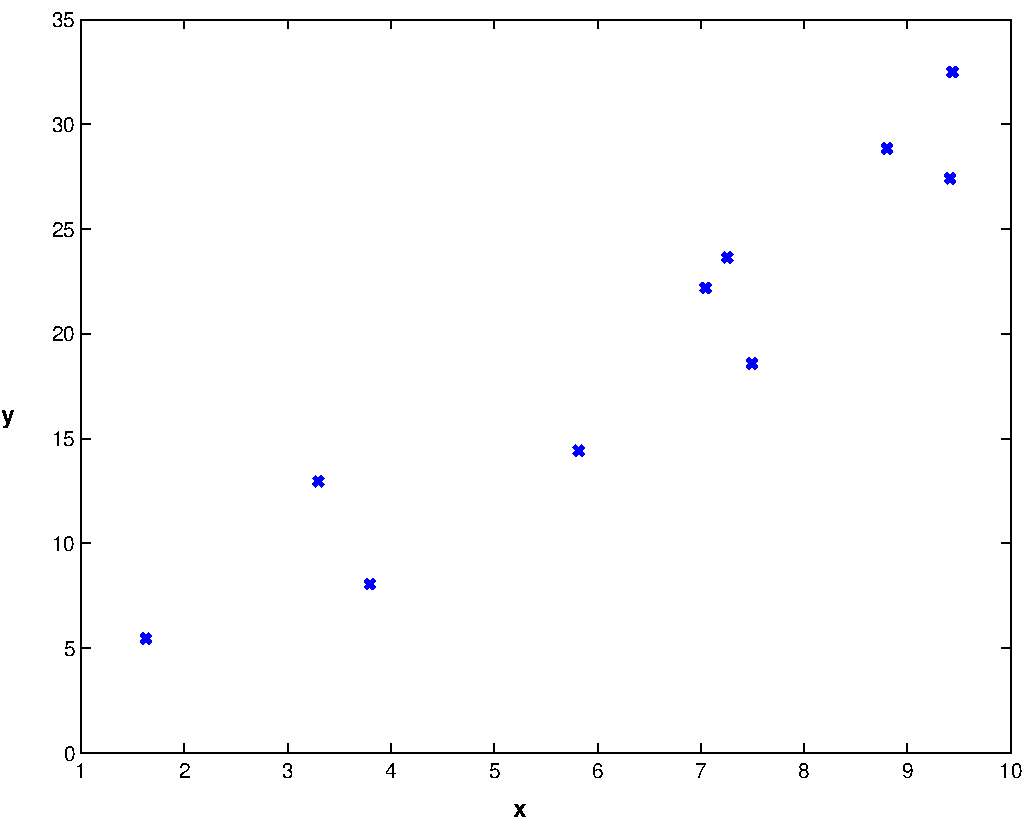
\includegraphics[width=.45\linewidth]{datacv}
\caption{Exemple of data set ( In this example $(\beta_0,\beta_1,\beta_2)=(1,3,0)$, $\sigma=3$ and $n=10$).}
\end{figure}

}
%%%%%%%%%%%%%%%%%%%%%%%%%%%%%%%%%%%%%%%%%%%%%%%%%%%%%%%%%
\frame{
\frametitle{The Model Selection Problem}

\begin{figure}[!h]
\begin{tabular}{cc}
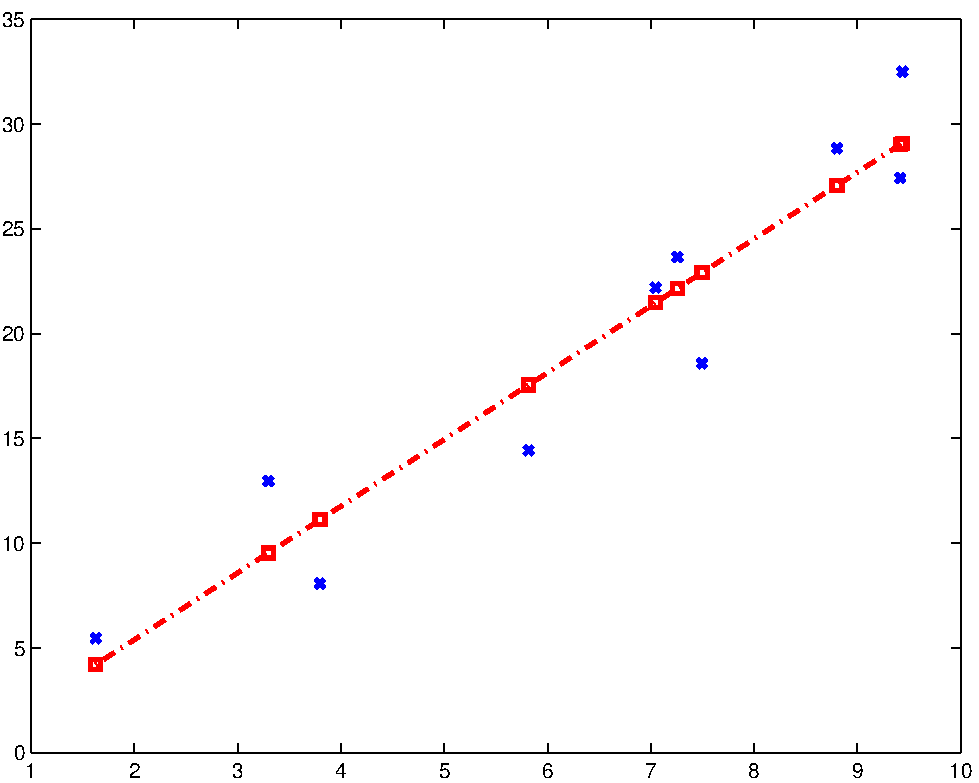
\includegraphics[width=.45\linewidth]{datacvline}&
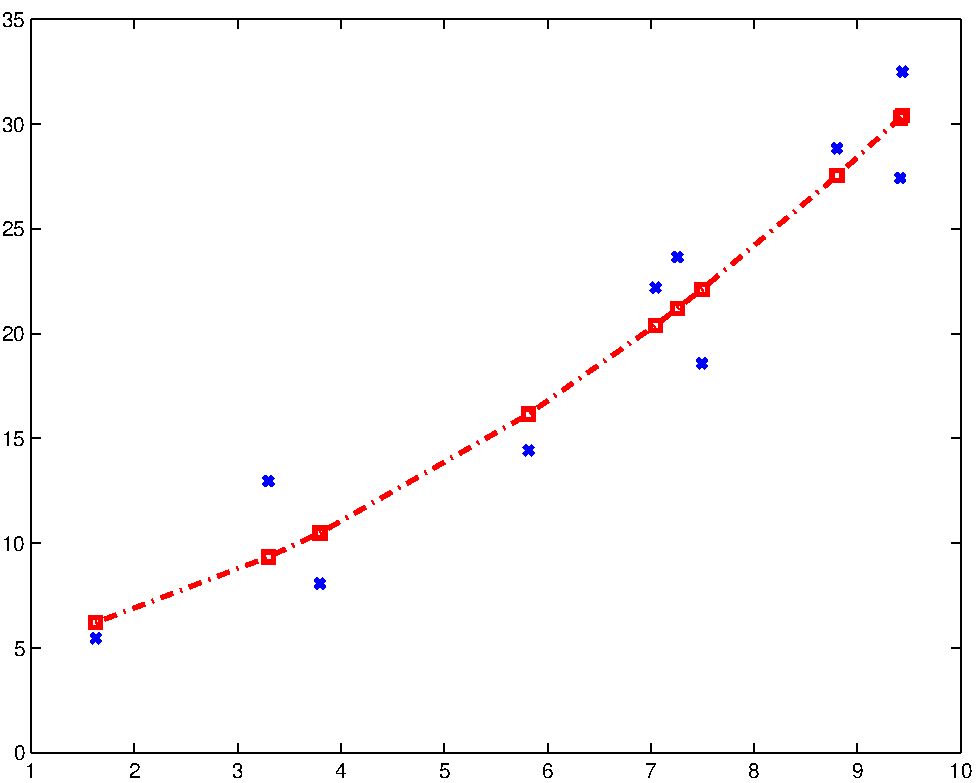
\includegraphics[width=.45\linewidth]{datacvquad}\\
Model A:  $\hat{y}=\hat{\beta}_1\ x+\hat{\beta}_0$ & Model B:  $\hat{y}=\hat{\beta}_2\  x^2+\hat{\beta}_1\  x+\hat{\beta}_0$ \\
\end{tabular}
\caption{The data points (blue cross) fitted assuming a linear model (left), and a quadratic model (right). Regression estimates are  $(\hat{\beta}_0,\hat{\beta}_1)=(-0.9802, 3.1866)$ for model A, and  $(\hat{\beta}_0,\hat{\beta}_1,\hat{\beta}_2)=(4.2380,0.8875, 0.1997)$ for model 2. \alert{Which model is the best ?}}
\end{figure}
}
%%%%%%%%%%%%%%%%%%%%%%%%%%%%%%%%%%%%%%%%%%%%%%%%%%%%%%%

%%%%%%%%%%%%%%%%%%%%%%%%%%%%%%%%%%%%%%%%%%%%%%%%%%%%%%%
\frame{
\frametitle{The Model Selection Problem}

\begin{itemize}
\item \alert{Which model is the best ?} = How well are you going to predict
future data drawn from the same
distribution?

\item As a prediction error, we can compute the average Residual Squared Error (RSE):
$$
\mathrm{PE} = \quad \frac{\mathrm{RSE}}{n}=\frac{\sum_{i=1}^{n} (y_i-\hat{y}_i)^2}{n}
$$
where $\hat{y}_i$ is the prediction by the model $\hat{y}_i=\hat{\beta}(x_i)$.

\item To start, $y_i$ is taken in the sample $\mathbf{z}$ (instead of a future response). In this case, the prediction error  is then called the \alert{apparent prediction error (APE)}  
\end{itemize}

}
%%%%%%%%%%%%%%%%%%%%%%%%%%%%%%%%%%%%%%%%%%%%%%%%%%%%%%%
\frame{
\frametitle{The Model Selection Problem}

\begin{figure}[!h]
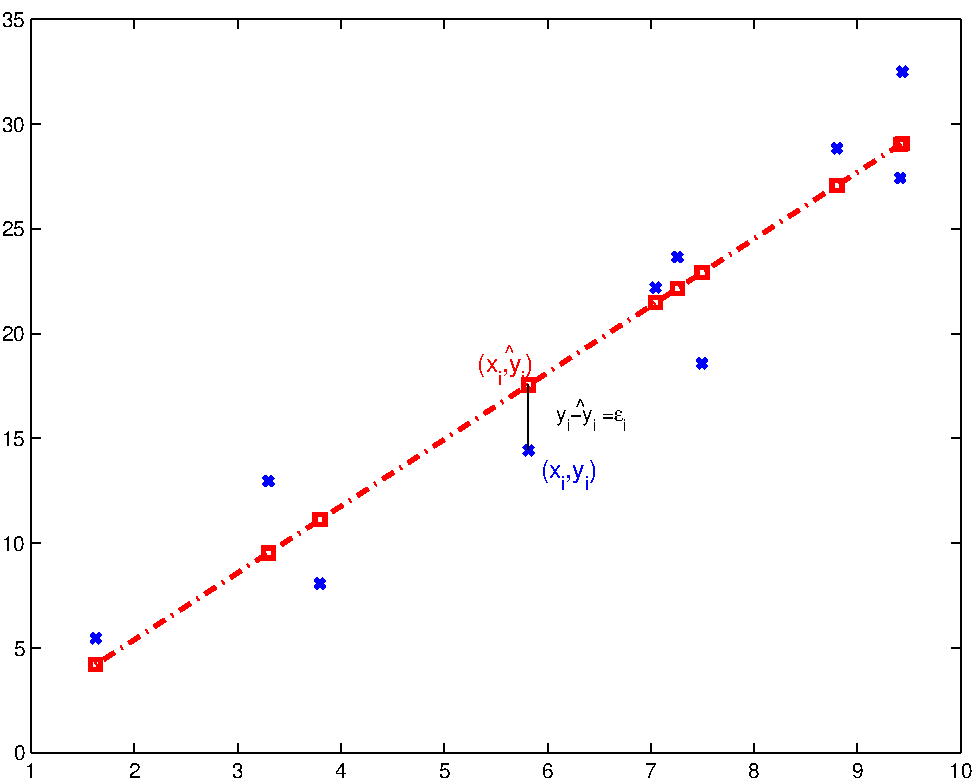
\includegraphics[width=.8\linewidth]{datacvlineb}
\end{figure}
}
%%%%%%%%%%%%%%%%%%%%%%%%%%%%%%%%%%%%%%%%%%%%%%%%%%%%%%%
\frame{
\frametitle{The Model Selection Problem}

For our two models:
\begin{itemize}

\item For model A,  the apparent prediction error is $7.1240$.

\item For model B, the apparent prediction error is $5.8636$

\end{itemize}

The apparent prediction error computed with model B is better (smaller) than
with the model A. Note that  the family of functions in B contains the ones defined in A. So B can capture more   variabilities in the data set $\mathbf{z}$, and can fit (in the sense of the APE)  better the observation $\mathbf{z}$.

\begin{itemize}

\item  But this is an \textit{apparent} prediction error. What is the prediction error for a new observation ? 

\item \alert{How to get a new sample to compute this prediction?}
\end{itemize}
}


%%%%%%%%%%%%%%%%%%%%%%%%%%%%%%%%%%%%%%%%%%%%%%%%%%%%%%%
\frame{
\frametitle{Cross-validation}

\begin{itemize}
\item For a more realistic estimate of the prediction error, we need a test sample different from the   training sample.

\

\item One way is to split the observation $\mathbf{z}$ into two sets, one for training and the other one for testing. 

\
\item Using  a part of the available observation to fit the model, and a different part to test in the computation of predication error is known as the cross-validation.  


\end{itemize}

}
\frame{
\frametitle{Simple and double cross-validation}

\begin{itemize}
\item \textbf{Simple cross-validation}. Divide the set $\mathbf{z}$ into two groups, one for \textit{training} and the other one for \textit{testing}. The parameters $\beta$ are estimated on the training data set. The cross-validation  is the prediction error  computed using the test sample.

\

\item \textbf{Double cross-validation}.  Models are generated for  both sub-samples, and then both equations are used to generate  cross-validation.

\end{itemize}

}
%%%%%%%%%%%%%%%%%%%%%%%%%%%%%%%%%%%%%%%%%%%%%%%%%%%%%%%
\frame{
\frametitle{K-Fold cross-validation}

\begin{beamercolorbox}[wd=\linewidth, rounded=true,shadow=true]{postit}
\begin{enumerate}
\item Split $\mathbf{z}$ into $K$ equal subsets $\mathbf{z}_k$

\

\item  Do $K$ times:
\begin{itemize}
\item Estimate the model $\beta_{(k)}$ on $\mathbf{z}_{(k)}=\lbrace \mathbf{z}_1, \cdot,\mathbf{z}_{k-1}, \mathbf{z}_{k+1}, \cdots,\mathbf{z}_{K} \rbrace $ 

\

\item Compute the prediction error $\mathrm{PE}(k)$ between the  test sample $\mathbf{z}_k$ and the predicted model by $\beta_{(k)}$.
\end{itemize}

\

\item Compute the  average of those $K$ prediction errors as the overall estimate of the prediction error 
$$
\mathrm{CV}=\frac{1}{K} \sum_{k=1}^{K} \mathrm{PE}(k)
$$
\end{enumerate}
\end{beamercolorbox}
}
%%%%%%%%%%%%%%%%%%%%%%%%%%%%%%%%%%%%%%%%%%%%%%%%%%%%%%%
\frame{
\frametitle{K-Fold cross-validation}
\begin{itemize}
\item The number $K$ of subsets depend on the size $n$ of the observation $\mathbf{z}$.

\

  \item For large datasets, even 3-Fold Cross Validation will be quite accurate.

\

\item For small datasets, we may have to use \textbf{leave-one-out} cross validation  where $K=n$.

\ 

\item \textbf{Multicross-validation} is an extension of double cross-validation. Double cross-validation procedures are repeated many times by randomly selecting sub-samples from the data set. 
\end{itemize}
}
%%%%%%%%%%%%%%%%%%%%%%%%%%%%%%%%%%%%%%%%%%%%%%%%%%%%%%%
\frame{
\frametitle{Cross-validation and parameter selection} 
\begin{itemize}
\item We just show how to perform model selection (i.e. choice of the number of parameters $p$ in the regression model).

\

\item Cross-validation can also be used for parameter estimation by  choosing the parameter value  which minimises the prediction error.

\

\item The cross-validation is computed using subsamples of  $\mathbf{z}$. An alternative consists in considering bootstrap samples. 

\end{itemize}
}
%%%%%%%%%%%%%%%%%%%%%%%%%%%%%%%%%%%%%%%%%%%%%%%%%%%%%%%
\frame{
\frametitle{Bootstrap estimates of the prediction error}


\begin{beamercolorbox}[wd=\linewidth, rounded=true,shadow=true]{postit}
\begin{enumerate}
\item Compute $B$ boostrap resamples $\mathbf{z}^{*}$ from the observation $\mathbf{z}$

\

\item Compute the model parameter $\beta^{*(b)}$ from  $\mathbf{z}^{*}$, and the corresponding prediction error PE$(b)$ with the testing observation being the original sample $\mathbf{z}$. 

\

\item Compute the  average of those $B$ prediction errors as the overall estimate of the prediction error 
$$
\mathrm{CV}_{boot}=\frac{1}{B} \sum_{b=1}^{B} \mathrm{PE}(b)
$$
\end{enumerate}
\end{beamercolorbox}

}
%%%%%%%%%%%%%%%%%%%%%%%%%%%%%%%%%%%%%%%%%%%%%%%%%%%%%%
\frame{
\frametitle{Bootstrap estimates of the prediction error}

\begin{itemize}
\item This bootstrap extension to cross-validation turns out to not work very well. But it can be improved.
 
\item Keep the record of the results from the previous procedure. Run a second experiment but choosing the bootstrap sample $\mathbf{z}^{*}$ itself as a test sample. Compute the difference of the two previous results (this difference is called optimism). This optimism is then added to the APE ( as a bias correction).

\item Which is best between CV and bootstrap alternatives is not really clear. 

\end{itemize}
}


%%%%%%%%%%%%%%%%%%%%%%%%%%%%%%%%%%%%%%%%%%%%%%%%%%%%%%
\frame{
\frametitle{Other estimates of  the prediction error}

\begin{itemize}
\item So far, we have define the PE using the average RSE. This is the prediction error measure used in cross-validation.

\item One can think of using other measures such as the  Bayesian Information Criterion (BIC)
$$
\frac{RSE}{n}+\log{n} \cdot p\hat{\sigma}^{2}/n 
$$

\item BIC penalises the model as  the number of parameter $p$ increases. It is a consistent criterion i.e. it chooses the good model as $n\rightarrow \infty$.

\item However, two drawbacks of the BIC compared to CV:
\begin{itemize}
\item you need an estimate  $\hat{\sigma}$.
\item you need the knowledge of $p$. 
\end{itemize} 

\end{itemize}
}
%%%%%%%%%%%%%%%%%%%%%%%%%%%%%%%%%%%%%%%%%%%%%%%%%%%%%%%
\frame{
\frametitle{Summary}

\begin{itemize}
\item Cross validation method applied to selection model (regression).

\

\item Other applications such as classification use the cross-validation. In this case, $y_i$ is a label  indicating the class. The prediction error is defined as a misclassification rate.   

\

\item Those methods  are very much used  in machine learning.
% (= area of artificial intelligence concerned with the development of techniques which allow computers to learn). 
% It is a method for creating computer programs by the analysis of data sets. It is also concerned with the algorithmic complexity of computational implementations. 


\end{itemize}

}



\end{document}
